%%%%%%%%%%%%%%%%%%%%%%%%%%%%%%%%%%%%%%%%%
% kaobook
% LaTeX Template
% Version 1.3 (December 9, 2021)
%
% This template originates from:
% https://www.LaTeXTemplates.com
%
% For the latest template development version and to make contributions:
% https://github.com/fmarotta/kaobook
%
% Authors:
% Federico Marotta (federicomarotta@mail.com)
% Based on the doctoral thesis of Ken Arroyo Ohori (https://3d.bk.tudelft.nl/ken/en)
% and on the Tufte-LaTeX class.
% Modified for LaTeX Templates by Vel (vel@latextemplates.com)
%
% License:
% CC0 1.0 Universal (see included MANIFEST.md file)
%
%%%%%%%%%%%%%%%%%%%%%%%%%%%%%%%%%%%%%%%%%

%----------------------------------------------------------------------------------------
%	PACKAGES AND OTHER DOCUMENT CONFIGURATIONS
%----------------------------------------------------------------------------------------

\documentclass[
	a4paper, % Page size
	fontsize=10pt, % Base font size
	twoside=true, % Use different layouts for even and odd pages (in particular, if twoside=true, the margin column will be always on the outside)
	%open=any, % If twoside=true, uncomment this to force new chapters to start on any page, not only on right (odd) pages
	%chapterentrydots=true, % Uncomment to output dots from the chapter name to the page number in the table of contents
	numbers=noenddot, % Comment to output dots after chapter numbers; the most common values for this option are: enddot, noenddot and auto (see the KOMAScript documentation for an in-depth explanation)
]{kaobook}

% Choose the language
\ifxetexorluatex
	\usepackage{polyglossia}
	\setmainlanguage{english}
\else
	\usepackage[english]{babel} % Load characters and hyphenation
\fi
\usepackage[english=british]{csquotes}	% English quotes

% Load packages for testing
\usepackage{blindtext}
%\usepackage{showframe} % Uncomment to show boxes around the text area, margin, header and footer
%\usepackage{showlabels} % Uncomment to output the content of \label commands to the document where they are used

% Load the bibliography package
\usepackage{kaobiblio}
\addbibresource{main.bib} % Bibliography file

% Load mathematical packages for theorems and related environments
\usepackage[framed=true]{kaotheorems}

% Load the package for hyperreferences
\usepackage{kaorefs}

% Load package for graphs
\usepackage{tikz}

% Load package for animations
\usepackage{graphicx, animate}

% Loadpackage and definitions for Diracs delta notation
\usepackage{mathtools}
\DeclarePairedDelimiter\bra{\langle}{\rvert}
\DeclarePairedDelimiter\ket{\lvert}{\rangle}
\DeclarePairedDelimiterX\braket[2]{\langle}{\rangle}{#1\,\delimsize\vert\,\mathopen{}#2}



\graphicspath{{examples/documentation/images/}{images/}} % Paths in which to look for images

\makeindex[columns=3, title=Alphabetical Index, intoc] % Make LaTeX produce the files required to compile the index

\makeglossaries % Make LaTeX produce the files required to compile the glossary
\newglossaryentry{computer}{
	name=computer,
	description={is a programmable machine that receives input, stores and manipulates data, and provides output in a useful format}
}

% Glossary entries (used in text with e.g. \acrfull{fpsLabel} or \acrshort{fpsLabel})
\newacronym[longplural={Frames per Second}]{fpsLabel}{FPS}{Frame per Second}
\newacronym[longplural={Tables of Contents}]{tocLabel}{TOC}{Table of Contents}

 % Include the glossary definitions

\makenomenclature % Make LaTeX produce the files required to compile the nomenclature

% Reset sidenote counter at chapters
%\counterwithin*{sidenote}{chapter}

%----------------------------------------------------------------------------------------

\begin{document}

%----------------------------------------------------------------------------------------
%	BOOK INFORMATION
%----------------------------------------------------------------------------------------

\title{Quantum Mechanics I}

\author[Adolfo Menéndez Rua]{Adolfo Menéndez Rúa}

\date{\today}

% \publishers{}

%----------------------------------------------------------------------------------------

\frontmatter % Denotes the start of the pre-document content, uses roman numerals

%----------------------------------------------------------------------------------------
%	OPENING PAGE
%----------------------------------------------------------------------------------------

%\makeatletter
%\extratitle{
%	% In the title page, the title is vspaced by 9.5\baselineskip
%	\vspace*{9\baselineskip}
%	\vspace*{\parskip}
%	\begin{center}
%		% In the title page, \huge is set after the komafont for title
%		\usekomafont{title}\huge\@title
%	\end{center}
%}
%\makeatother

%----------------------------------------------------------------------------------------
%	COPYRIGHT PAGE
%----------------------------------------------------------------------------------------

\makeatletter
\uppertitleback{\@titlehead} % Header

\lowertitleback{
	\textbf{Disclaimer}\\
	You can edit this page to suit your needs. For instance, here we have a no copyright statement, a colophon and some other information. This page is based on the corresponding page of Ken Arroyo Ohori's thesis, with minimal changes.

	\medskip

	\textbf{No copyright}\\
	\cczero\ This book is released into the public domain using the CC0 code. To the extent possible under law, I waive all copyright and related or neighbouring rights to this work.

	To view a copy of the CC0 code, visit: \\\url{http://creativecommons.org/publicdomain/zero/1.0/}

	\medskip

	\textbf{Colophon} \\
	This document was typeset with the help of \href{https://sourceforge.net/projects/koma-script/}{\KOMAScript} and \href{https://www.latex-project.org/}{\LaTeX} using the \href{https://github.com/fmarotta/kaobook/}{kaobook} class.

	The source code of this book is available at:\\\url{https://github.com/fmarotta/kaobook}

	(You are welcome to contribute!)

	\medskip

	\textbf{Publisher} \\
	First printed in May 2019 by \@publishers
}
\makeatother

%----------------------------------------------------------------------------------------
%	DEDICATION
%----------------------------------------------------------------------------------------

% \dedication{
% 	I would rather have questions that can't be answer than answers that can't be question.\\
% 	\flushright -- Richard P. Feynman
% }

\dedication{
Coding is easy, algebra is easy, calculus is easy, physics is imposible.\\
	\flushright -- Rajamani S. Narayanan
}
%----------------------------------------------------------------------------------------
%	OUTPUT TITLE PAGE AND PREVIOUS
%----------------------------------------------------------------------------------------

% Note that \maketitle outputs the pages before here

\maketitle

%----------------------------------------------------------------------------------------
%	PREFACE
%----------------------------------------------------------------------------------------

\chapter*{Preface}
\addcontentsline{toc}{chapter}{Preface} % Add the preface to the table of contents as a chapter

This book is written with my lack of knowledge in LaTeX and my notes token from Professor Rajamani S. Narayanan course on Quantum Mechanics at Florida International University. During this pages I am going to learn how to manage LaTeX as an useful tool while I am dealing with understand the world of the Quantum Mechanics. 

I will start with some Classical Mechanics to understand how the Quantum Mechanics appeared in the first place. 

I also want to thank to Abel Rosado who helps me and teaches me on how to use this template.

% I am of the opinion that every \LaTeX\xspace geek, at least once during 
% his life, feels the need to create his or her own class: this is what 
% happened to me and here is the result, which, however, should be seen as 
% a work still in progress. Actually, this class is not completely 
% original, but it is a blend of all the best ideas that I have found in a 
% number of guides, tutorials, blogs and tex.stackexchange.com posts. In 
% particular, the main ideas come from two sources:

% \begin{itemize}
% 	\item \href{https://3d.bk.tudelft.nl/ken/en/}{Ken Arroyo Ohori}'s 
% 	\href{https://3d.bk.tudelft.nl/ken/en/nl/ken/en/2016/04/17/a-1.5-column-layout-in-latex.html}{Doctoral 
% 	Thesis}, which served, with the author's permission, as a backbone 
% 	for the implementation of this class;
% 	\item The 
% 		\href{https://github.com/Tufte-LaTeX/tufte-latex}{Tufte-Latex 
% 			Class}, which was a model for the style.
% \end{itemize}

% The first chapter of this book is introductory and covers the most
% essential features of the class. Next, there is a bunch of chapters 
% devoted to all the commands and environments that you may use in writing 
% a book; in particular, it will be explained how to add notes, figures 
% and tables, and references. The second part deals with the page layout 
% and design, as well as additional features like coloured boxes and 
% theorem environments.

% I started writing this class as an experiment, and as such it should be 
% regarded. Since it has always been intended for my personal use, it may
% not be perfect but I find it quite satisfactory for the use I want to 
% make of it. I share this work in the hope that someone might find here 
% the inspiration for writing his or her own class.

\begin{flushright}
	\textit{Adolfo Menéndez Rua}
\end{flushright}

\index{preface}

%----------------------------------------------------------------------------------------
%	TABLE OF CONTENTS & LIST OF FIGURES/TABLES
%----------------------------------------------------------------------------------------

\begingroup % Local scope for the following commands

% Define the style for the TOC, LOF, and LOT
%\setstretch{1} % Uncomment to modify line spacing in the ToC
%\hypersetup{linkcolor=blue} % Uncomment to set the colour of links in the ToC
\setlength{\textheight}{230\hscale} % Manually adjust the height of the ToC pages

% Turn on compatibility mode for the etoc package
\etocstandarddisplaystyle % "toc display" as if etoc was not loaded
\etocstandardlines % "toc lines" as if etoc was not loaded

\tableofcontents % Output the table of contents
\listoffigures % Output the list of figures

% Comment both of the following lines to have the LOF and the LOT on different pages
\let\cleardoublepage\bigskip
\let\clearpage\bigskip

\listoftables % Output the list of tables

\endgroup

%----------------------------------------------------------------------------------------
%	MAIN BODY
%----------------------------------------------------------------------------------------

\mainmatter % Denotes the start of the main document content, resets page numbering and uses arabic numbers
\setchapterstyle{kao} % Choose the default chapter heading style

\setchapterpreamble[u]{\margintoc}
\chapter{Classical Mechanics}
\labch{intro}

\section{The Two-Body Problem}

As it is showed in \reffig{draw_1} we have two bodies with masses $m_1$ and $m_2$ and they interact with a force unknown.

We can define their positions as: $\vec{r_1}$ and $\vec{r_2}$ and the separation between them as $ \vec{r} =\vec{r_1} - \vec{r_2} $

I said that the force is unknown but we know:

\begin{itemize}
    \item $F_{12} = - F_{21}$
    \item The force only depends on the distance between the two bodies and the direction is the line between them, i.e. $F = f(r)\hat{r}$  \sidenote[][3cm]{$\hat{r}=\frac{\Vec{r}}{|\vec{r}|}$}
    \item The force can be defined as a central force so we can define a potential as: $f(r)=\frac{d\nu(r)}{dr}$
\end{itemize}

% First Figure

\begin{marginfigure}[-3cm]
\begin{tikzpicture}

\draw[->] (0,0) -- (2,2);
\filldraw[black] (1,1) circle (0pt) node [anchor=west]{$\vec{r_1}$};

\draw[->] (0,0) -- (-2,2);
\filldraw[black] (-1,1) circle (0pt) node [anchor=east]{$\vec{r_2}$};

\filldraw[black] (2,2) circle (2pt) node [anchor=west]{$m_1$};
\filldraw[black] (-2,2) circle (2pt) node [anchor=east]{$m_2$};
\filldraw[black] (0,0) circle (2pt) node [anchor=north]{O};
\filldraw[->] (2,2) -- (-1.9,2);
\filldraw[black] (0,2) circle (0pt) node [anchor=south]{$\vec{r}$};

\draw[->] (2,2.2) -- (1,2.2);
\filldraw[black] (1.5,2.2) circle (0pt) node [anchor=south]{$\vec{F_{21}}$};

\draw[->] (-2,2.2) -- (-1,2.2);
\filldraw[black] (-1.5,2.2) circle (0pt) node [anchor=south]{$\vec{F_{12}}$};

\end{tikzpicture}
\caption[Two bodies interacting with some force]{Two bodies interacting with some force at some time}
\labfig{draw_1}
\end{marginfigure}


Using Newton 3rd Law we can explain the movement of this two objects by two equations:

\begin{equation}
    \label{newton_1}
    m_1 \frac{d^2\vec{r_1}}{dt^2} = f(r)\hat{r}
\end{equation}

\begin{equation}
    \label{newton_2}
    m_2 \frac{d^2\vec{r_2}}{dt^2} = - f(r)\hat{r}
\end{equation}

Let's add \ref{newton_1} and \ref{newton_2}, this is going to be useful later.

\begin{equation}
    \label{newton_1+2}
    m_1\frac{d^2\vec{r_1}}{dt^2} + m_2\frac{d^2\vec{r_2}}{dt^2} = 0
\end{equation}

We can not get anything from \ref{newton_1} and \ref{newton_2}, so we are going to transform this equations into something we can use to resolve them. First, we define the center of mass and their derivatives among time:

\begin{equation}
    \label{center_of_mass}
    \vec{r_{CM}}=\frac{m_1\vec{r_1} + m_2\vec{r_2}}{m_1 + m_2}
\end{equation}

\begin{equation}
    \label{velocity_center_of_mass}
    \vec{v_{CM}}=\frac{d}{dt}\vec{r_{CM}} = \frac{1}{m_1 + m_2}\left[m_1\frac{d\vec{r_1}}{dt} + m_2\frac{d\vec{r_2}}{dt}  \right]
\end{equation}

\begin{equation}
    \label{aceleration_center_of_mass}
    \vec{a_{CM}}=\frac{d}{dt}\vec{v_{CM}} = \frac{1}{m_1 + m_2}\left[m_1\frac{d^2\vec{r_1}}{dt^2} + m_2\frac{d^2\vec{r_2}}{dt^2}  \right]
\end{equation}

If we look at \ref{aceleration_center_of_mass} we can see something equal to the left term on \ref{newton_1+2} so we can say that the acceleration of the center of mass is zero, i.e. $\vec{a_{CM}} = 0$.

This mean that the center of mass moves with a constant velocity and we can define it's move as:

\begin{equation}
    \label{center_of_mass_2}
    \vec{r_{CM}}= R_{CM} + V_{CM} \cdot t
\end{equation}

Where $R_{CM}$ and $V_{CM}$ are constants defined by initial conditions. Knowing this we can make a change of the coordinates with the next assumption:

\begin{equation}
    \label{change_of_coordinates_1}
    \vec{r_{1}} = \vec{r_{1}'} + \vec{r_{CM}}
\end{equation}

\begin{equation}
    \label{change_of_coordinates_2}
    \vec{r_{2}} = \vec{r_{2}'} + \vec{r_{CM}}
\end{equation}

% Second Figure : Change of the coordinates

\begin{marginfigure}[-3cm]
\begin{tikzpicture}

\draw[->] (0,0) -- (2,2);
\filldraw[black] (1,1) circle (0pt) node [anchor=west]{$\vec{r_1}$};

\draw[->] (0,0) -- (-2,2);
\filldraw[black] (-1,1) circle (0pt) node [anchor=east]{$\vec{r_2}$};

\filldraw[black] (2,2) circle (2pt) node [anchor=west]{$m_1$};
\filldraw[black] (-2,2) circle (2pt) node [anchor=east]{$m_2$};
\filldraw[black] (0,0) circle (2pt) node [anchor=north]{O};
\filldraw[->] (2,2) -- (-1.9,2);
\filldraw[black] (0,2.1) circle (0pt) node [anchor=south]{$\vec{r}$};

\draw[->] (2,2.2) -- (1,2.2);
\filldraw[black] (1.5,2.2) circle (0pt) node [anchor=south]{$\vec{F_{21}}$};

\draw[->] (-2,2.2) -- (-1,2.2);
\filldraw[black] (-1.5,2.2) circle (0pt) node [anchor=south]{$\vec{F_{12}}$};

% Change
\draw[->, blue] (0,0) -- (-1.8,0.45);
\filldraw[blue] (-2,0.5) circle (2pt) node [anchor=east]{${R_{CM}}$};
\filldraw[blue] (-1.25,0.25) circle (0pt) node [anchor=north]{${\vec{r_{CM}}(t = 0)}$};

\filldraw[blue] (0,2) circle (2pt) node [anchor=north]{${\vec{r_{CM}}(t)}$};

\draw[->, blue] (0,1.9) -- (1.75,1.9);
\filldraw[blue] (1,1.8) circle (0pt) node [anchor=north]{$\vec{r_1}'$};

\draw[->, blue] (0,1.9) -- (-1.75,1.9);
\filldraw[blue] (-1,1.8) circle (0pt) node [anchor=north]{$\vec{r_2}'$};

\end{tikzpicture}
\caption[Two-body problem with new coordinates]{Two-body problem with the new coordinates}
\labfig{draw_2}
\end{marginfigure}

Now let's calculate the new center of mass $\vec{r_{CM}'}$ using \ref{change_of_coordinates_1} and \ref{change_of_coordinates_2}

\begin{equation}
    \label{cm_prima}
    \begin{split}
    \vec{r_{CM}'} & = \frac{m_1\vec{r_1'}+ m_2\vec{r_2'}}{m_1+m_2} \\
                  & = \frac{1}{m_1 + m_2} \left[ m_1(\vec{r_1}-\vec{r_{CM}}) + m_2(\vec{r_2}-\vec{r_{CM}})\right] \\
                  & = \vec{r_{CM}} - \frac{1}{m_1+m_2}\left[\vec{r_{CM}}(m_1+ m_2)\right]\\
                  & = \vec{r_{CM}} - \vec{r_{CM}} = 0 \hspace{2mm} \sidenote[][2mm]{The professor demonstrate the same but with the expression for $\Vec{r_{CM}}$, this is just another way I prefer.}
    \end{split}
\end{equation}

As it should be, our new center of mass is the origin for all time because our new referential system is moving with the center of mass. From this assumptions and using the definition of the new center of mass above we can get a new system of equations.

\begin{equation}
\label{sys_eq_1}
    \left\{
    \begin{array}{l}
        m_1\vec{r_1'} + m_2\vec{r_2'} = 0 \\
        \vec{r_1'} - \vec{r_2'} = \vec{r}
    \end{array}
    \right. =>
    \left\{
    \begin{array}{l}
        \vec{r_1'} = \frac{m_2\vec{r}}{m_1+m_2} \\
        \vec{r_2'} = \frac{-m_1\vec{r}}{m_1+m_2}
    \end{array}
    \right.
\end{equation}

 We use what we obtain from \ref{sys_eq_1} in \ref{newton_1} and \ref{newton_2}. We can do this because the force does not change in this coordinates because only depend on r and this magnitude is still the same, i.e. $\vec{r}=\vec{r'}$.

\begin{equation}
\label{sys_eq_sol}
    m \frac{d^2\vec{r}}{dt^2} = f(r) \vec{r}
\end{equation}

\marginnote[-2mm]{m is the reduce mass define as: \newline $ m = \frac{m_1 m_2}{m_1 + m_2}$}
\marginnote[1cm]{Normally we can use $m \approx m_2$ when $m_1 >> m_2$, some examples of this are Sun and Earth or proton and electron. With real values:\newline $m_{S-E} = \frac{m_S m_E}{m_S + m_E} \approx 5.96998 \cdot 10^{24}kg \aprox m_E$, where $m_S = 2 \cdot10^{30}kg, m_E = 5.97\cdot 10^{24}kg$}

We get the same equation from both equations.This expression will be useful to resolve the problem later.

\section{The Angular Momentum}
\labsec{does}

We define the angular momentum as:

\begin{equation}
\label{ang_mom}
    \vec{L} = \vec{r} \times \vec{p} = m \vec{r} \times \frac{d\Vec{r}}{dt}
\end{equation}

We want to now how this quantity changes among time.

\begin{equation}
\label{ang_mom_dt}
    \frac{d\vec{L}}{dt} = m \frac{\vec{dr}}{dt} \times \frac{d\vec{r}}{dt} + m \vec{r} \times \frac{d^2\vec{r}}{dt^2} = 0 + \vec{r} \times f(r) \hat{r} = 0
\end{equation}

The law of the conservation of angular momentum says that the angular momentum of a system remains constant unless an external rotational force (torque) acts upon it.

As we just demonstrate the angular momentum vector is constant and we can redefine it as:

\begin{equation}
\label{ang_mom_2}
    \vec{L} = L \hat{z}
\end{equation}

The decision of L going through the $\hat{z}$ direction is going to be very resourceful.



\section{Cylindrical coordinates}
\labsec{does}

We need to choose a coordinate system to resolve the problem. Our best option is to choose cylindrical coordinates.

\begin{equation}
\label{cylindrical}
\begin{split}
    &\vec{r} = \rho \hat{\rho} + z \hat{z} \\
    &\frac{d\vec{r}}{dt} = \frac{d\rho}{dt}\hat{\rho} + \rho \frac{d\phi}{dt}\hat{\phi}+\frac{dz}{dt}\hat{z}
\end{split}
\end{equation}

\begin{marginfigure}[-2cm]
    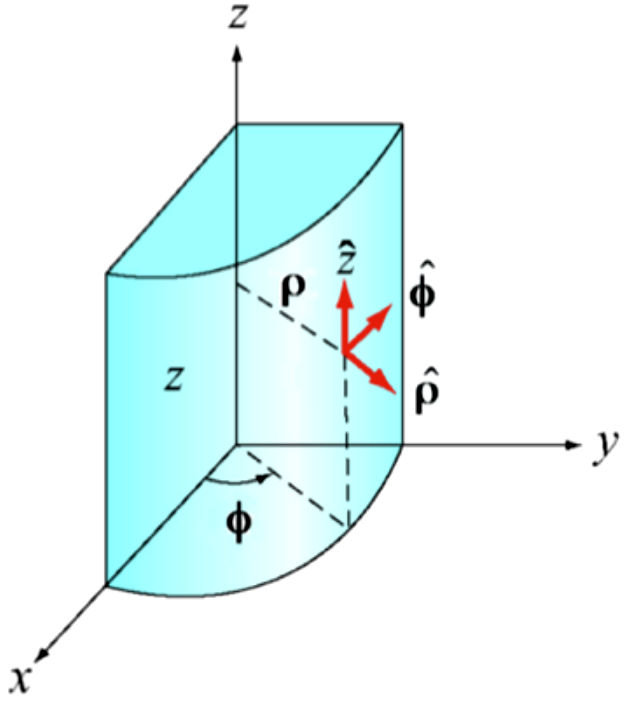
\includegraphics{cylindrical}
    \caption[Cylindrical coordinates]{Cylindrical coordinates.\\       \url{https://www.researchgate.net/publication/334148643/figure/fig1/AS:775915730649091@1562004134358/Diagram-of-a-standard-cylindrical-coordinate
    -system-with-radius-r-azimuth-ph-and-height.jpg}}
    \labfig{margincylind}
\end{marginfigure}

If we use \ref{cylindrical} in \ref{ang_mom_dt} we can look at $\Vec{L}$ components

\begin{equation}
\label{ang_cyl}
\begin{split}
    \vec{L} = & m (\rho \hat{\rho} + z \hat{z}) \times \left(\frac{d\rho}{dt}\hat{\rho} + \rho \frac{d\phi}{dt}\hat{\phi}+\frac{dz}{dt}\hat{z}\right) = \\
              & - m z \rho \frac{d\phi}{dt}\hat{\rho} + m\left(z\frac{d\rho}{dt}-\rho\frac{dz}{dt}\right)\hat{\phi}+ m \rho^2\frac{d\phi}{dt}\hat{z}
    \end{split}
\end{equation}

Using the definition in \ref{ang_mom_2} and our new equation we get 4 different equations if we compare the angular momentum in each direction.

\begin{equation}
    \label{sys_ang_mom}
    \begin{split}
    &1. \hspace{30} L \neq 0 \\
    &2. \hspace{30}m z \rho \frac{d\phi}{dt} = 0 \\
    &3. \hspace{30}m \left( z \frac{d\rho}{dt} - \rho \frac{dz}{dt} \right) = 0 \\
    &4. \hspace{30}m \rho^2\frac{d\phi}{dt} = L
    \end{split}
\end{equation}

This gives you a lot of information:

\begin{itemize}
    \item $m \neq 0$
    \item $\rho \neq 0$
    \item $\frac{d\phi}{dt} \neq 0$
    \item $z = 0$
    \item $\frac{d\phi}{dt} = \frac{L}{m\rho^2}$

\end{itemize}

This equations not only give us a fixed value of z it also give us that in the system we choose the value for z is 0 for all time. We also can get a relation between the derivative of $\phi$ and $\rho$. We will use this later to resolve the problem.

If z=0 we can redefine $\vec{r}$ from \ref{cylindrical}.

\begin{equation}
    \label{from_r_to_rho}
    \begin{split}
        &\vec{r} = \vec{\rho} = \rho\hat{\rho} \\
        &\frac{d^2\vec{\rho}}{dt^2} = \left[ \frac{d^2\rho}{dt^2} -\rho\left(\frac{d\phi}{dt}\right)^2 \right]\hat{\rho} + \left[2\frac{d\rho}{dt}\frac{d\phi}{dt} +\rho\frac{d^2\phi}{dt^2} \right]\hat{\phi}
    \end{split}
\end{equation}

We loose the therm that goes in the $\hat{\phi}$ direction because is zero. We can see this in two different ways:

\begin{itemize}
    \item Now our force $F = f(r)\hat{r} = f(\rho)\hat{\rho}$ because \ref{from_r_to_rho} so the second derivative of $\Vec{\rho}$ only can have a component in the $\hat{\rho}$ direction.
    \item If we calculate what we have in the $\hat{\phi}$ component using some notions in derivatives and \ref{sys_ang_mom} we would get 0  \sidenote[][2cm]{$2\frac{d\rho}{dt}\frac{d\phi}{dt} +\rho\frac{d^2\phi}{dt^2} = \frac{d}{dt}\left(\rho^2\frac{d\phi}{dt}\right)= \frac{d}{dt}\left(\frac{L}{m}\right) = 0$, because both L and m are constants.}
\end{itemize}



If we return to \ref{sys_eq_sol} with everything we learnt we can get something very interesting, an scalar equation.

\begin{equation}
    \label{scalar_eq}
    m\left[ \frac{d^2\rho}{dt^2}-\rho\left(\frac{d\phi}{dt}\right)^2 \right] = f(\rho)
\end{equation}

We get a scalar equation with two variables $\rho$ and $\phi$, but we can use \ref{sys_ang_mom} as before and reduce everything to a scalar equation with one variable.

\begin{equation}
    \label{solution_1}
    m\left[ \frac{d^2\rho}{dt^2}-\rho\frac{L^2}{m^2\rho^4}\right] = f(\rho) = -\frac{d\nu(\rho)}{d\rho}
\end{equation}

We can put everything in one side of the equation and multiply both sides by a factor $\frac{d\rho}{dt}$

\begin{equation} \label{solution_2}
    \begin{split}
    & m \frac{d^2\rho}{dt^2} \frac{d\rho}{dt} - \frac{d}{dt} \left( \frac{L^2}{m\rho^3} \right) + \frac{d}{dt} \frac{d\nu(\rho)}{d\rho} = 0 \\
    & \frac{d}{dt} \left(\frac{1}{2}m\left(\frac{d\rho}{dt}\right)^2+\frac{L^2}{2m\rho^2}+ \nu(\rho) \right) = 0
    \end{split}
\end{equation}

We know that this magnitude inside the brackets is constant during the time. This magnitude is the total energy, E, and we can divide it three:

\begin{description}
    \item [Linear Kinetic Energy] $K = \frac{1}{2}m(\frac{d\rho}{dt})^2$
    \item [Angular Kinetic Energy] $K_{\alpha} = \frac{L^2}{2m\rho^2}$
    \item [Potential Energy] $\nu(\rho) = \frac{-k}{r}$   \sidenote[][2mm]{This is what we usually use as potential energy because it appears in nature, for example, Newton Gravity Law and Coulomb Law}
\end{description}

\section{Potential wells}
\labsec{does}

We are going to study the angular kinetic energy and the potential energy (both are functions of $\rho$), we call the addition of these two energies \textbf{Effective potential}

\begin{marginfigure}
    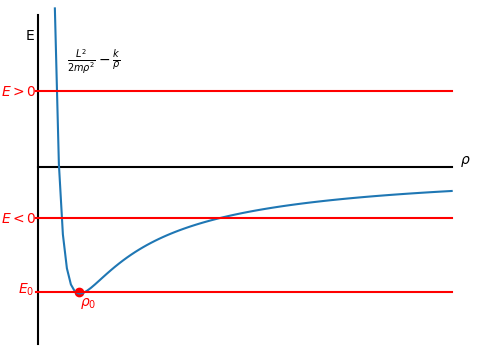
\includegraphics{images/general.png}
    \caption[Effective Potential]{Effective Potential}
    \labfig{marginfigeff}
\end{marginfigure}

In \reffig{marginfigeff} we can see many things:

\begin{itemize}
    \item The function have a minimum that is the lowest possible total energy because the linear kinetic energy is always greater or equal to 0, i. e. $K\geq0$. This energy represents a circular motion.

    \item If we have a higher energy but still negative, the movement is an elliptical motion with two values that are the nearest and the furthest point in the ellipse.

    \item If the energy is positive the motion is no more a close orbit and we say that the motion is an hyperbola.

    \item If the total energy is 0, the motion is in the limit between a close and an open orbit and the movement is a parable.
\end{itemize}

In the next section we are going to give real values to this magnitudes.

\section{Physical Examples}
\labsec{does}

\textbf{1. Earth-Sun problem:} If we take the Earth and the Sun as our two bodies we need to know some values. We already know the reduce mass from the previous section. The k value of the potential energy is $ k = GM_Sm_E$, we know this value from Newton´s Gravitational Law.

\begin{itemize}
    \item $m_E = 2 \cdot 10{30} kg$
    \item $M_S = 5.97\cdot 10^{24} kg$
    \item $G = 6.67 \cdot 10^{11} Nm^2/kg^2$
\end{itemize}

The total energy of the system is:

\begin{equation}
\label{energy_E-S}
    E = \frac{1}{2}m\left(\frac{d\rho}{dt}\right)^2+\frac{L^2}{2m\rho^2}+ \frac{ - G M_S m_E}{\rho}
\end{equation}

We can see in \reffig{marginfig_ES} that if we represent $U = K_{\alpha}+\nu(\rho)$ against $\rho$ we get a similar function to the one in \reffig{marginfigeff}, but we can see in the axis that we have large energies and distances. That is reasonable if we think that we are working with massive objects as planets.

\begin{marginfigure}
    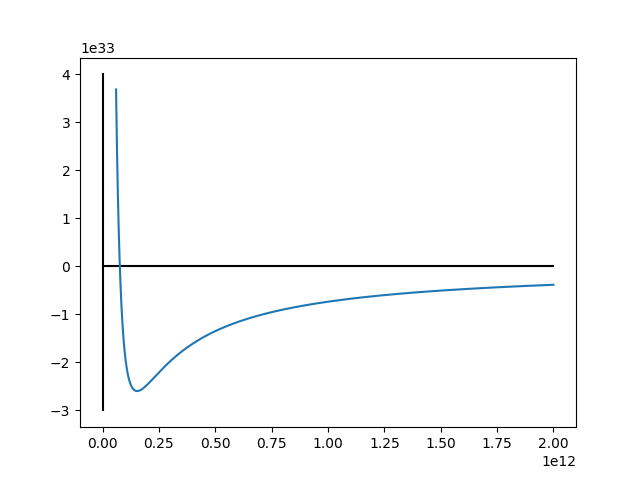
\includegraphics{images/E-S_Potential_Well.png}
    \caption[Effective Potential for Earth-Sun]{Effective Potential for Earth-Sun}
    \labfig{marginfig_ES}
\end{marginfigure}

We can calculated now the minimum energy the Earth-Sun system can have in which, the Earth would orbit by a circular motion.

To calculate this energy we need to calculate first the value of $\rho$ for this minimum energy ($\rho_{min}$). This value can be found by matching the first derivative of the function U($\rho$) to 0

\begin{equation}
    \label{Der_Ueff}
    \begin{split}
    &\frac{dU}{d\rho} = \frac{d}{d\rho}\left[ \frac{L^2}{2m\rho^2}+ \frac{ - G M_S m_E}{\rho}\right]=\\
    &\frac{-L^2}{m\rho^3}+\frac{G M_S m_E}{\rho^2}
    \end{split}
\end{equation}

If we match \ref{Der_Ueff} to 0 and solve for $\rho$ we get $\rho_{min}$

\begin{equation}
    \label{rho_min_ES}
    \begin{split}
    &\frac{-L^2}{m\rho^3}+\frac{G M_S m_E}{\rho^2} = 0\\
    &\frac{G M_S m_{E}^2\rho - L^2}{m_E\rho^3} = 0\\
    &\rho_{min} = \frac{L^2}{G M_S m_{E}^2}
    \end{split}
\end{equation}

If we use \ref{rho_min_ES} in \ref{energy_E-S} knowing that our minimum energy implies K = 0, we get the minimum energy possible.

\begin{equation}
    \label{energy_min_ES}
    E = -\frac{1}{2}\frac{G^2M_{S}^2m_{E}^3}{L^2} = -\frac{1}{2}\frac{G M_S m_{E}}{\rho_{min}}=\frac{1}{2}\nu(\rho_{min})
\end{equation}

If we look into the equation \ref{energy_min_ES} we can demonstrate that the minimum energy is a half of the potential energy.

\textbf{2. Electron-Proton problem:} If we take a proton and an electron we can do the same as before knowing their masses. The problem is very similar, just with different conditions. The reduce mass is going to be the mass of the electron because it is much less than the mass of the proton.

\begin{itemize}
    \item $m_e = 9.11 \cdot 10{-31} kg$
    \item $m_p = 1.67\cdot 10^{-27} kg$
    \item $G = 6.67 \cdot 10^{11} kg$
\end{itemize}

The total energy of the system is:

\begin{equation}
\label{energy_E-P_mass}
    E = \frac{1}{2}m\left(\frac{d\rho}{dt}\right)^2+\frac{L^2}{2m\rho^2}+ \frac{ - G M_p m_e}{\rho}
\end{equation}

\begin{marginfigure}
    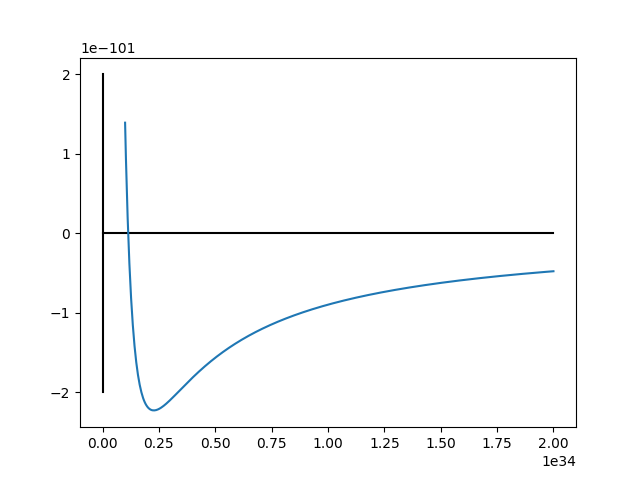
\includegraphics{images/E-P_Potential_Well.png}
    \caption[Effective Potential for Electron-Proton]{Effective Potential for Electron-Proton}
    \labfig{marginfig_EP}
\end{marginfigure}

We can see in \reffig{marginfig_EP} that if we represent $U = K_{\alpha}+\nu(\rho)$ against $\rho$ we get a similar function to \reffig{marginfigeff}, but if we focus in the axis we can see that we have very low energies. That is reasonable if we think that we are working with particles that have very little mass.

I'm not going to do all we did before. In this case, because the energy is so low, is not interesting to study it. But there is another potential that affects electron and proton, the electric potential.

\textbf{3. Electron-Proton problem with Electric Potential:} In this case we need to define the charges of the proton and the electron. Also we need to define a new potential, where $ k = \frac{Ze^2}{4\pi\epsilon_0} $ where Z is the atomic number, e is the charge of the electron  \sidenote[][1mm]{This value was discovered by the Nobel Price Robert Andrews Millikan by his experiment called: Millikan oil drop experiment} and $\epsilon_0$ is the permittivity of free space.

\begin{itemize}
    \item $e = 1.6 \cdot 10^{-19} \cdot 10{30} kg$
    \item $\epsilon_0 = 8.85 \cdot 10^{-12} kg$
\end{itemize}

The total energy of the system is:

\begin{equation}
\label{energy_E-P_elec}
    E = \frac{1}{2}m\left(\frac{d\rho}{dt}\right)^2+\frac{L^2}{2m\rho^2}+ \frac{-Ze^2}{4\pi\epsilon_0\rho}
\end{equation}

If we look at \reffig{marginfig_EP_elec} and compare it with \reffig{marginfig_EP} we can see a high difference in the Energy scale. This means that the electrical force is much stronger than the gravitational force.

\begin{marginfigure}
    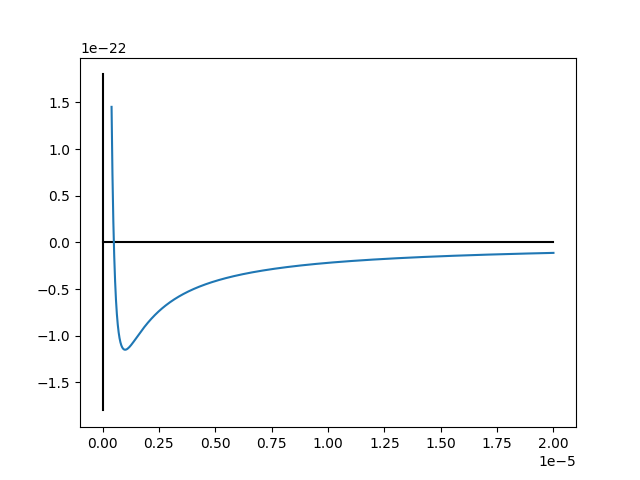
\includegraphics{images/E-P_elec_Potential_Well.png}
    \caption[Effective Potential for Electron-Proton (Electric Potential)]{Effective Potential for Electron-Proton (Electric Potential)}
    \labfig{marginfig_EP_elec}
\end{marginfigure}

We can calculated now the minimum energy the Electron-Proton system can have in which, the electron would orbit by a circular motion around the proton.

To calculate this energy we need to calculate first the value of $\rho$ for this minimum energy ($\rho_{min}$). This value can be found by matching the first derivative of the function in \reffig{marginfig_ES} to 0

\begin{equation}
    \label{Der_Ueff}
    \begin{split}
    &\frac{dU}{d\rho} =\frac{d}{d\rho}\left[ \frac{L^2}{2m\rho^2}+ \frac{ -Ze^2}{\rho}\right]=\\
    &\frac{-L^2}{m\rho^3}+\frac{-Ze^2}{4\pi\epsilon_0\rho^2}
    \end{split}
\end{equation}

If we match \ref{Der_Ueff} to 0 and solve for $\rho$ we get $\rho_{min}$.

\begin{equation}
    \label{rho_min}
    \begin{split}
    &\frac{-L^2}{m\rho^3}+\frac{Ze^2}{4\pi\epsilon_0\rho^2} = 0\\
    &Ze^2m\rho - 4 L^2\pi\epsilon_0 = 0\\
    &\rho_{min} = \frac{4L^2\pi\epsilon_0}{Ze^2m}
    \end{split}
\end{equation}

We can also get the square of the angular momentum as a function of $\rho$.

\begin{equation}
    \label{L_min}
    L^2 = \frac{m\rho_{min}Ze^2}{4\pi\epsilon_0}
\end{equation}

Now, we have two different expressions for the minimum energy.

\begin{equation}
    \label{E_min_EP}
    \begin{split}
    &1) E_{min} = -\frac{Ze^2}{8\pi\epsilon_0\rho^2}\\
    &2) E_{min} = -\frac{Z^2e^4m}{2(4\pi\epsilon_0)^2}\frac{1}{L^2}
    \end{split}
\end{equation}

Looking at the first expression we have the same as the Earth-Proton problem, we get that the minimum energy is half of the potential energy.

The second expression is even more interesting because after measure the length wave of light from an hydrogen atom, Bohr discovered that L was proportional to the energy level of the atom (n). Later they found that the relation is:

\begin{equation}
    \label{L_min}
    L = hn
\end{equation}
\marginnote{h is known as the Plank constant. \\
$h\approx 6.63\cdot10^{-34}$}

\section{Rotation and angular momentum}
\labsec{does}

To finished this chapter we are going to talk about something that is very interesting and purely mathematical.

We know that the rotation in 3D is not commutative and we also know that the definition of the module of $\vec{L}$ is

\begin{equation}
    \label{module_L}
    L^2=|\Vec{L}|^2=L_{x}^2+L_{y}^2+L_{z}^2
\end{equation}

This means that we can have multiple solutions for L using rotations.

We define a vector $\ket{j,m}$ where j is the representation and m is the bases vector of the representation. Then we get this relations:

\begin{equation}
\label{jm_vec}
    \begin{split}
        & L^2 \ket{j,m} = j(j+1)\ket{j,m}\\
        & L_z \ket{j,m} = m \ket{j,m}
    \end{split}
\end{equation}

I'm not proving anything, we will derive and talk about these in more detail in chapter 9.

% The \Class{kaobook} class focuses more about the document structure than
% about the style. Indeed, it is a well-known \LaTeX\xspace principle that
% structure and style should be separated as much as possible (see also
% \vrefsec{doesnot}). This means that this class will only provide
% commands, environments and in general, the opportunity to do things,
% which the user may or may not use. Actually, some stylistic matters are
% embedded in the class, but the user is able to customise them with ease.

% The main features are the following:

% \begin{description}
% 	\item[Page Layout] The text width is reduced to improve readability
% 	and make space for the margins, where any sort of elements can be
% 	displayed.
% 	\item[Chapter Headings] As opposed to Tufte-Latex, we provide a
% 	variety of chapter headings among which to choose; examples will be
% 	seen in later chapters.
% 	\item[Page Headers] They span the whole page, margins included, and,
% 	in twoside mode, display alternatively the chapter and the section
% 	name.\sidenote[][-2mm]{This is another departure from Tufte's
% 	design.}
% 	\item[Matters] The commands \Command{frontmatter},
% 	\Command{mainmatter} and \Command{backmatter} have been redefined in
% 	order to have automatically wide margins in the main matter, and
% 	narrow margins in the front and back matters. However, the page
% 	style can be changed at any moment, even in the middle of the
% 	document.
% 	\item[Margin text] We provide commands \Command{sidenote} and
% 	\Command{marginnote} to put text in the
% 	margins.\sidenote[][-2mm]{Sidenotes (like this!) are numbered while
% 	marginnotes are not}
% 	\item[Margin figs/tabs] A couple of useful environments is
% 	\Environment{marginfigure} and \Environment{margintable}, which, not
% 	surprisingly, allow you to put figures and tables in the margins
% 	(\cfr \reffig{marginmonalisa}).
% 	\item[Margin toc] Finally, since we have wide margins, why don't add
% 	a little table of contents in them? See \Command{margintoc} for
% 	that.
% 	\item[Hyperref] \Package{hyperref} is loaded and by default we try
% 	to add bookmarks in a sensible way; in particular, the bookmarks
% 	levels are automatically reset at \Command{appendix} and
% 	\Command{backmatter}. Moreover, we also provide a small package to
% 	ease the hyperreferencing of other parts of the text.
% 	\item[Bibliography] We want the reader to be able to know what has
% 	been cited without having to go to the end of the document every
% 	time, so citations go in the margins as well as at the end, as in
% 	Tufte-Latex. Unlike that class, however, you are free to customise
% 	the citations as you wish.
% \end{description}

% \begin{marginfigure}[-5.5cm]
% 	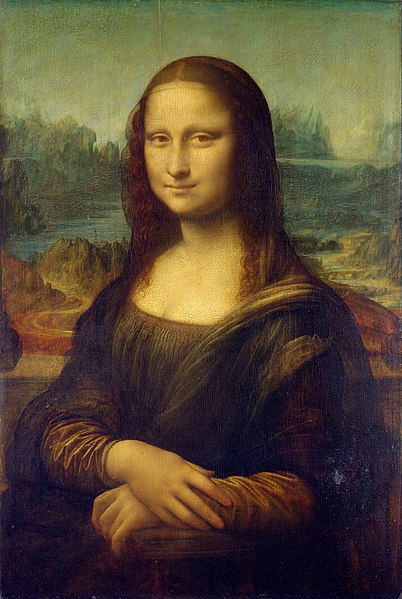
\includegraphics{monalisa}
% 	\caption[The Mona Lisa]{The Mona Lisa.\\
% 	\url{https://commons.wikimedia.org/wiki/File:Mona_Lisa,_by_Leonardo_da_Vinci,_from_C2RMF_retouched.jpg}}
% 	\labfig{marginmonalisa}
% \end{marginfigure}

% The order of the title pages, table of contents and preface can be
% easily changed, as in any \LaTeX\ document. In addition, the class is
% based on \KOMAScript's \Class{scrbook}, therefore it inherits all the
% goodies of that.

% \section{What This Class Does Not Do}
% \labsec{doesnot}

% As anticipated, further customisation of the book is left to the user.
% Indeed, every book may have sidenotes, margin figures and so on, but
% each book will have its own fonts, toc style, special environments and
% so on. For this reason, in addition to the class, we provide only
% sensible defaults, but if these features are not needed, they can be
% left out. These special packages are located in the \Path{style}
% directory, which is organised as follows:

% \begin{description}
% 	\item[kao.sty] This package contains the most important definitions
% 	of macros and specifications of page layout. It is the heart of the
% 	\Class{kaobook}.
% 	\item[kaobiblio.sty] Contains commands to add citations and
% 	customise the bibliography.
% 	\item[packages.sty] Loads additional packages to decorate the
% 	writing with special contents (for instance, the \Package{listing}
% 	package is loaded here as it is not required in every book). There
% 	are also defined some useful commands to print the same words always
% 	in the same way, \eg latin words in italics or \Package{packages} in
% 	verbatim.
% 	\item[kaorefs.sty] Some useful commands to manage labeling and
% 	referencing, again to ensure that the same elements are referenced
% 	always in a consistent way.
% 	\item[environments.sty] Provides special environments, like boxes.
% 	Both simple and complex environments are available; by complex we
% 	mean that they are endowed with a counter, floating and can be put
% 	in a special table of contents.\sidenote[][-2mm]{See
% 	\vrefch{mathematics} for some examples.}
% 	\item[theorems.sty] The style of mathematical environments.
% 	Actually, there are two such packages: one is for plain theorems,
% 	\ie the theorems are printed in plain text; the other uses
% 	\Package{mdframed} to draw a box around theorems. You can plug the
% 	most appropriate style into its document.
% \end{description}

% \marginnote[2mm]{The audacious users might feel tempted to edit some of
% these packages. I'd be immensely happy if they sent me examples of what
% they have been able to do!}

% In the rest of the book, I shall assume that the reader is not a novice
% in the use of \LaTeX, and refer to the documentation of the packages
% used in this class for things that are already explained there.
% Moreover, I assume that the reader is willing to make minor edits to the
% provided packages for styles, environments and commands, if he or she
% does not like the default settings.

% \section{How to Use This Class}

% Either if you are using the template from
% \href{http://latextemplates.org/template/kaobook}{latextemplates}, or if
% you cloned the GitHub
% \href{https://www.github.com/fmarotta/kaobook}{repository}, there are
% infinite ways to use the \Class{kaobook} class in practice, but we will
% discuss only two of them. The first is to find the \Path{main.tex} file
% which I used to write this book, and edit it; this will probably involve
% a lot of text-deleting, copying-and-pasting, and rewriting. The second
% way is to start almost from scratch and use the \Path{skeleton.tex}
% file, which is a cleaned-up version of the \Path{main.tex}; even if you
% choose the second way, you may find it useful to draw inspiration from
% the \Path{main.tex} file.

% To compile the document, assuming that its name is \Path{main.tex}, you
% will have to run the following sequence of commands:

% \begin{lstlisting}[style=kaolstplain,linewidth=1.5\textwidth]
% pdflatex main # Compile template
% makeindex main.nlo -s nomencl.ist -o main.nls # Compile nomenclature
% makeindex main # Compile index
% biber main # Compile bibliography
% makeglossaries main # Compile glossary
% pdflatex main # Compile template again
% pdflatex main # Compile template again
% \end{lstlisting}

% You may need to compile the template some more times in order for some
% errors to disappear. For any support requests, please ask a question on
% \url{tex.stackexchange.org} with the tag \enquote{kaobook}, open an
% issue on GitHub, or contact the author via e-mail.


\pagelayout{wide} % No margins
% \addpart{Class Options, Commands and Environments}
\pagelayout{margin} % Restore margins

\setchapterpreamble[u]{\margintoc}
\chapter{Waves}
\labch{options}

Waves are some example of classical mechanics, where we have a function that propagates among time. During this chapter we will define their properties and their relation with quantum mechanics.

\section{The wave function}

We define a function that propagates in one dimension (x) among the time (t).

\begin{equation}
\label{wave_function}
    \psi(x,t) = e^{i(kx-\omega t)} 
\end{equation}

Where $\omega$ is the angular velocity of propagation and k is the wave number. We are working with complex numbers but the solution to the function can not be a complex number because it has a physical meaning.


We can define the phase as the function inside the exponential.

\begin{equation}
    \label{phase_def}
    \phi(x,t) = kx-\omega t
\end{equation}

If we set $\phi$ constant we will be "riding" the wave.

\section{Energy and momentum}

We are interested in see what happens among time and space in this function, so we are going to differentiate.

\begin{equation}
    \label{diff_wave}
    \begin{split}
        &\frac{d}{dt}\psi(x,t) = -i\omega e^{i(kx-\omega t)}\\
        &\frac{d}{dx}\psi(x,t) = ik e^{i(kx-\omega t)}\\
    \end{split}
\end{equation}

We choose to work with one dimension but everything could have been done in three dimensions just using x and k as vectors.

Now we are going to do some assumptions. 

\begin{equation}
    \label{Energy_Momentum}
    \begin{split}
        &E = \hbar \omega = i\hbar\frac{d}{dt}\\
        &P = \hbar k = -i\hbar\Vec{\nabla} 
    \end{split}
\end{equation}

We can define the energy as some constant ($\hbar$) times the frequency. If we use the same constant and multiply it to the wave number we get something with units of momentum, so we can call it momentum. 

The second term in both expression is what we call energy and momentum operator.  

We now from classical mechanics that energy and momentum are related.

\begin{equation}
    \label{Energy(momentum)}
    E = \frac{P\cdot P}{2m} + \nu
\end{equation}

In the previous chapter we got the expression of the energy, with which we can get the position at any time if the are some initial conditions given.

In the same way, if $\psi(\vec{x},0)$ is given we can compute $\psi(\vec{x},t)$ using the energy and momentum operators.

\section{P(x) function I: Definition and properties}

Experimentally describe a particle at rest. If we plot the position measure we will get different answers for the same experiment. 

\begin{figure}[h]
    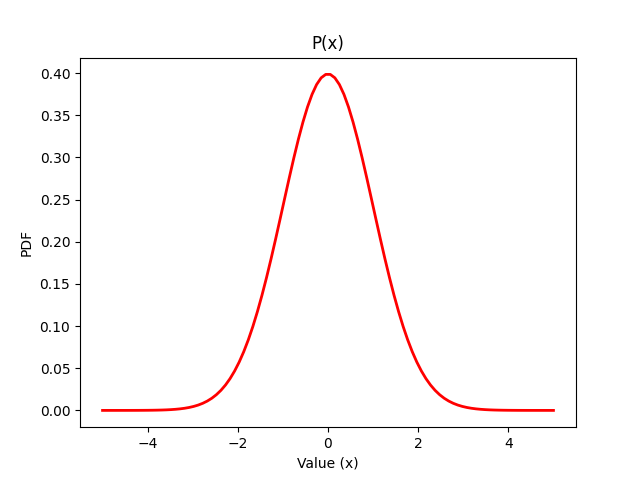
\includegraphics{images2/PDF_function.png}
    \caption{Normal distribution for mean=0 and sigma=1, to simulate a experiment measured by different people}
    \label{PDF_function}
\end{figure}
    

In wave mechanics P(x) should be interpreted as $\psi^2(x,0)$.

\marginnote[-1cm]{*Uncertainty is not probability}

We can define P(x) as a Gaussian distribution with an undetermined constant.

\begin{equation}
\label{P(x)_def}
    P(x) = A e^{-\frac{x^2}{2 \sigma^2}}
\end{equation}

We also make the next choice to define P(x):

\begin{equation}
\label{int_P(x)_def}
    \int_{-\infty}^{\infty}P(x) dx = 1
\end{equation}

We are going to ignore the constant for now to keep things simpler.

\begin{equation}
\label{int_P(x)_alpha}
    I = \int_{-\infty}^{\infty}e^{-\alpha x^2} dx 
\end{equation}

\marginnote[]{$ \Re[\alpha]> 0$, $\alpha \in \mathbb{C}$}

We need to resolve the integral of P(x), but it is not a direct integral and is difficult to resolve it directly. Luckily we can use a trick to resolve this integral.

\begin{equation}
\label{int_P(x)_r}
\begin{split}
    &I^2 = \left[\int_{-\infty}^{\infty}e^{-\alpha x^2} dx\right] \left[\int_{-\infty}^{\infty}e^{-\alpha y^2} dy\right] =\\
    & =  \int_{-\infty}^{\infty}e^{-\alpha(x^2+y^2)}dxdy = \\
    & =  \int_{0}^{2\pi}d\theta\int_{0}^{\infty}re^{-\alpha r^2}dr = \\
    & = 2\pi \frac{-1}{2\alpha} \left[ e^{-\alpha r^2} \right]_{0}^{\infty} = \frac{\pi}{\alpha}  
\end{split}
\end{equation}

\marginnote[-3cm]{dxdy = rdrd$\theta$}

If we want \ref{int_P(x)_def} to be true we need to normalize it using the result from \ref{int_P(x)_r}.

\begin{equation}
A = \sqrt{\frac{\alpha}{\pi}} \hspace{1cm} where \hspace{1cm} \alpha = \frac{1}{2\sigma^2}
\end{equation}

We get that the final value of our P(x) function is:

\begin{equation}
\label{P(x)_final_def}
    P(x) = \frac{1}{\sqrt{2\pi}\sigma} e^{-\frac{x^2}{2 \sigma^2}}
\end{equation}

We will continue with this later but first, we need to define Fourier Series.

\section{Fourier Series}

If we have a periodic function with length L so f(x) = f(x+L), then we can rewrite any function in this way:

\begin{equation}
\label{fourier}
    f(x) = \sum_{k=0}^{N} \tilde{f}_{k}\psi_{k}(x)
\end{equation}

Where $\psi_k(x)$ follow the next statements.

\begin{equation}\label{psi_k_fourier}
    \begin{split}
        &1)\hspace{2pt} \psi_k(x) = \frac{1}{\sqrt{L}}e^{i\frac{2\pi k}{L}x} \\ 
        &2) \int_0^L \psi_{k}^{\star}(x)\psi_{k'}(x) = \delta_{k,k'}
    \end{split}
\end{equation}

\marginnote[-1cm]{$\delta$ is a Dirac delta}

Using Fourier analysis we can rewrite our wave function into:

\begin{equation}
    \label{fourir_psi}
    \psi(x) = \sqrt{P(x)} = \int_{-\infty}^{\infty} \tilde{\psi}(k)e^{ikx}dk 
\end{equation}

If now we set some equations for $\psi(x)$.

\begin{equation}
    \label{rules_psi_fourier}
    \begin{split}
        &1) \hspace{2pt} Dom[\psi(x)]= \left( \frac{-L}{2},\frac{L}{2} \right) \\
        &2) \hspace{2pt} \psi(\frac{L}{2})=\psi(\frac{-L}{2})\\
        &3) \hspace{2pt} \psi(x) = e^{ikx}=e^{i\frac{2\pi n}{L}x}
    \end{split}
\end{equation}

We defined a orthogonal function $g_n$.

\begin{equation}
    \label{gn_def}
    \begin{split}
        & g_n(x) = \frac{1}{\sqrt{L}}e^{i\frac{2\pi}{L}nx}\\
        & \int_{\frac{-L}{2}}^{\frac{L}{2}}g_{n}^{\star}(x)g_{l}(x) dx = \frac{1}{L}\int_{\frac{-L}{2}}^{\frac{L}{2}} e^{i\frac{2\pi x}{L}(l-n)}dx = \delta_{l,n} 
    \end{split}
\end{equation}

\marginnote[-1cm]{$\delta_{l,n}$ is called Kronecker delta, this function is 1 when l = n and 0 for any other values}

We can use this function to rewrite $\psi(x)$

\begin{equation}
    \label{psi_gn_def} 
\begin{split}
    &\psi(x) = \frac{1}{\sqrt{L}}\sum_{n=-\infty}^{\infty}\Tilde{\psi}_n g_n(x)\\
    &\psi(x) = \frac{1}{2\pi}\sum_{n=-\infty}^{\infty} \frac{2\pi}{L}e^{i\frac{2\pi n}{L}x}\Tilde{\psi}_n
    \end{split}
\end{equation}

The last expression in \ref{psi_gn_def} is a Riemann sum so we can turn that expression into an integral.

\begin{equation}
    \label{psi_gn_final} 
\psi(x) = \frac{1}{2\pi} \int_{-\infty}^{\infty} \Tilde{\psi}(k)e^{ikx}dk
\end{equation}

We can find also an expression for $\Tilde{\psi}_n$.

\begin{equation}
    \label{til_psi_def_int} 
\begin{split}
    & \int_{\frac{-L}{2}}^{\frac{L}{2}} \psi(x) g_l^{\star}(x) dx =
    \\
    & = \frac{1}{\sqrt{L}} \sum_{-\infty}^{\infty} \Tilde{\psi}_n\int_{\frac{-L}{2}}^{\frac{L}{2}} g_n(x) g_l^{\star}(x) dx =
    \\
    & = \frac{1}{\sqrt{L}} \sum_{-\infty}^{\infty} \Tilde{\psi}_n \delta_{n,l} = \frac{1}{\sqrt{L}} \Tilde{\psi}_l
    \\
    & \Tilde{\psi}_l = \sqrt{L} \int_{\frac{-L}{2}}^{\frac{L}{2}} \psi(x) g_l^{\star}(x) dx
    \\
    & \Tilde{\psi}_l = \int_{\frac{-L}{2}}^{\frac{L}{2}} \psi(x) e^{-i\frac{2\pi l}{L}x} dx
    \end{split}
\end{equation}

If we extend to the limit where L approximate infinity we can get a general solution for $\tilde{\psi}(x)$.

\begin{equation}
    \label{2.20}
    \Tilde{\psi}(k) = \int_{-\infty}^{\infty} \psi(x) e^{-ikx} dx
\end{equation}

We have two different relations between $\psi(x)$ and $\tilde{\psi}(k)$, we need to make sure this two relations make sense together. To do this we are going to use \ref{2.20} and \ref{psi_gn_final}.

\begin{equation}
    \label{eq_2.21} 
\begin{split}
    & \psi(x) = \frac{1}{2\pi} \int_{-\infty}^{\infty} \left[ \int_{-\infty}^{\infty} \psi(y)e^{-iky}dy \right]e^{ikx}dk = 
    \\
    & = \int_{-\infty}^{\infty} \psi(y) \left[ \frac{1}{2\pi} \int_{-\infty}^{\infty} e^{ik(x-y)}dk\right]dy 
    \\
    & \psi(x) = \int_{-\infty}^{\infty} \psi(y) \delta(x-y) dy
    \end{split}
\end{equation}

The last equation we get from \ref{eq_2.21} is the definition of the Dirac delta function itself so we prove that both expressions we have are right.

\section{P(x) function II: $\psi(x)$ and $\tilde{\psi}(k)$}

We recover the equation \ref{P(x)_final_def} and know we get $\psi(x)$ remembering that $\psi^2(x) = P(x)$.

\begin{equation}
    \label{2.22}
    \psi(x) = \sqrt{P(x)} = \frac{1}{(2\pi\sigma^2)^{\frac{1}{4}} } e^{-\frac{x^2}{4\sigma^2}}
\end{equation}

We can also define $\Tilde{\psi}(k)$ with \ref{2.20}. 

\begin{equation}
    \label{2.23}
    \Tilde{\psi}(k) = \frac{1}{(2\pi\sigma^2)^{\frac{1}{4}} } \int_{-\infty}^{\infty} e^{\frac{-x^2}{4\sigma^2}-ikx}dx
\end{equation}

This integral is not easy to resolve, but we can get something similar to \ref{int_P(x)_alpha} and we already know the solution for that integral.

\begin{equation}
    \label{eq_2.24} 
    \begin{split}
    & \frac{x^2}{4\sigma^2}+ikx = \frac{1}{4\sigma^2}[x^2+4i\sigma^2 k x] = 
    \\
    & = \frac{1}{4\sigma^2}[(x+2i\sigma^2k)^2+4\sigma^4k^2]
    \\
    & e^{\frac{-x^2}{4\sigma^2}-ikx} = e^{-\sigma^2k^2}e^{-\frac{1}{4\sigma^2}(x+2i\sigma^2k)^2}
    \end{split}
\end{equation}

This expression can be used in \ref{2.23} to resolve the integral doing a variable change ($\tau = x+2i\sigma^2k$).

\begin{equation}
    \label{2.23}
    \Tilde{\psi}(k) = \frac{1}{(2\pi\sigma^2)^{\frac{1}{4}} } e^{-\sigma^2k^2} \int_{-\infty}^{\infty} e^{-\frac{\tau^2}{4\sigma^2}} d\tau
\end{equation}

\marginnote[]{We are not going to explain why $\infty+2i\sigma^2k = \infty$ and $-\infty+2i\sigma^2k = -\infty$, so the limits do not change. This can be prove with some complex analysis.}

Now we can resolve this integral because we already know the solution from \ref{int_P(x)_alpha}

\begin{equation}
    \label{2.23}
    \Tilde{\psi}(k) = \frac{1}{(2\pi\sigma^2)^{\frac{1}{4}} } e^{-\sigma^2k^2} \sqrt{4\sigma^2\pi} = 2^{\frac{3}{4}}\pi^{\frac{1}{4}}\sigma^{\frac{1}{2}} e^{-\sigma^2k^2}
\end{equation}

\section{Free particle}

If we set up the problem as a particle.

For t = 0:
    \begin{itemize}
        \item x = 0
        \item v = 0
    \end{itemize}

Then x(t) = 0. Also if E or p are given instead of v we can resolve the problem for x(t) 

If we interpret the free particle as a wave, using the knowledge from section 2.2 we will find a equation that describe the motion of the wave. First, we want to find a relation between w and k. We can get this equation using \ref{Energy_Momentum} and \ref{Energy(momentum)}. Because we are working with a free particle $\nu = 0$


\begin{equation}
    \label{2.27}
    \omega = \frac{\hbar k^2}{2m}
\end{equation}

The motion function can be found also using \ref{Energy_Momentum} and \ref{Energy(momentum)} 

\begin{equation}
    \label{2.28}
    \left(i\hbar\frac{d}{dt} \right)\psi = \frac{1}{2m}\left(-i\hbar\frac{d}{dx} \right)^2 \psi 
\end{equation}

We define P(x,0) as a gaussian function as we did in previous chapters.

\begin{equation}
    \label{2.29}
    P(x,0) = \frac{1}{\sqrt{2\pi\sigma^2}}e^{-\frac{x^2}{2\sigma^2}} 
\end{equation}

This P(x,t) function is what we called intensity of the wave, the question now is: if the wave is free ($\psi=\psi(x,t)$), what is P(x,t) ?  

We know from the previous chapter the solutions for $\psi(x,0)$ and $\Tilde{\psi}(x,0)$ when P(x,0) is a gaussian. 

\begin{equation}
    \label{2.30}
    \psi(x,0) = \frac{1}{\sqrt[4]{2\pi\sigma^2}} e^{\frac{x^2}{4\sigma^2}}
\end{equation} 

\begin{equation}
    \label{2.31}
    \tilde{\psi}(k) = 2^\frac{3}{4} \pi^\frac{1}{4} \sigma^\frac{1}{2} e^{-\sigma^2 k^2} 
\end{equation} 

If  $\psi(x,0)$ is interpreted as amplitude at x, $\tilde{\psi}(k)$ can be interpreted as amplitude at k. Also, we can define a intensity of k where $P(k) = \tilde{\psi}^2(k)$

\begin{figure}[h]
    \centering
    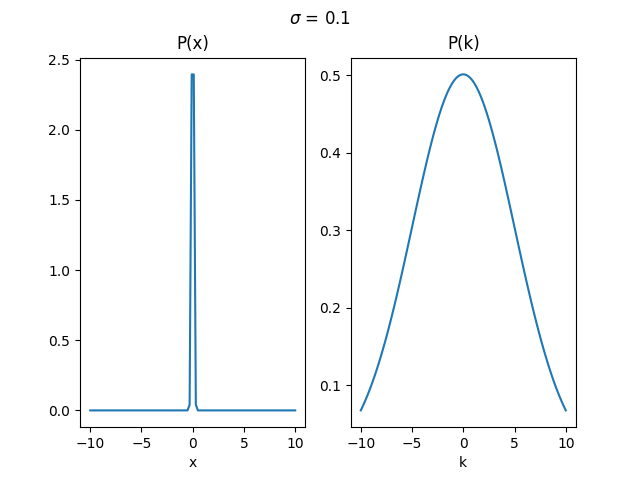
\includegraphics{images2/P_x&P_k_sigma=0.1.png}
    \caption{P(x) and P(k) for $\sigma$ = 0.1.}
    \labfig{sigma01}
\end{figure}

\begin{figure}[H]
    \centering
    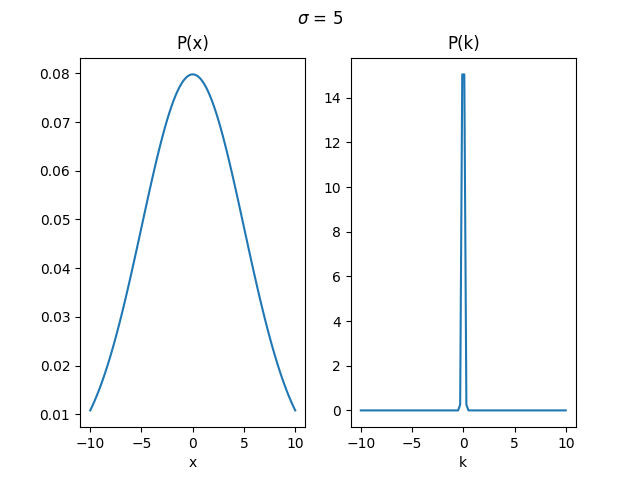
\includegraphics{images2/P_x&P_k_sigma=5.png}
    \caption{P(x) and P(k) for $\sigma$ = 5.}
    \labfig{sigma5}
\end{figure}

In this page we can see two different figures. In \reffig{sigma01} we have a very accurate result for the x value and a more deviated value for k while in \reffig{sigma5} is completely the opposite. This is a preamble to the uncertainty principle, however we still haven´t talk about quantum physics, this is just wave mechanics.


We need to get the expression among the time.

\begin{equation}
    \label{2.32}
    \psi(x,t) = \frac{1}{2\pi}\int_{-\infty}^{\infty} 2^\frac{3}{4} \pi^\frac{1}{4} \sigma^\frac{1}{2} e^{-\sigma^2 k^2} e^{ikx} e^{-i\frac{\hbar k^2}{2m}t} dk
\end{equation} 

This integral is not easy to resolve so we need to work the exponent.

\begin{equation}
    \label{2.33}
    \begin{split}
        & - \sigma^2 k^2 - i \frac{\hbar k^2}{2m} t + ikx = \\
        & = - (\sigma^2 + \frac{i\hbar t}{2m})k^2 + ikx = \\
        & = - (\sigma^2 + \frac{i\hbar t}{2m}) (k^2 - \frac{ikx}{\sigma^2 + \frac{i\hbar t}{2m}}) = \\
        & = - (\sigma^2 + \frac{i\hbar t}{2m}) (k-\frac{ix}{2(\sigma^2 + \frac{i\hbar t}{2m})})^2 + \frac{x^2}{4(\sigma^2 + \frac{i\hbar t}{2m})^2}
    \end{split}
\end{equation}

We get a similar exponent to the ones we work with where $\alpha = - (\sigma^2 + \frac{i\hbar t}{2m})$ and my variable is $\tau = k - \frac{ix}{2(\sigma^2+\frac{i\hbar t}{2m})}$

Using this to resolve \ref{2.32} we can get a final expression for $\psi(x,t)$.

\begin{equation}
    \label{2.34}
    \begin{split}
        &\psi(x,t) = \frac{1}{2\pi} 2^\frac{3}{4} \pi^\frac{1}{4} \sigma^\frac{1}{2} \frac{\pi^\frac{1}{2}}{(\sigma^2 + \frac{i\hbar t}{2m})^\frac{1}{2}} e^{\frac{-x^2}{4(\sigma^2 + \frac{i\hbar t}{2m})}} = \\
        & = \left( \frac{\sigma^2}{2\pi(\sigma^2 + \frac{i\hbar t}{2m})^2}\right)^{\frac{1}{4}}e^{-\frac{x^2}{4(\sigma^2 + \frac{i\hbar t}{2m})}}
    \end{split}
\end{equation} 

We can calculate P(x,t) knowing $\psi$(x,t).

\begin{equation}
    \label{2.35}
    \begin{split}
        & P(x,t) = \frac{\sigma}{\sqrt{2\pi}(\sigma^4 + \frac{\hbar^2t^2}{4m^2})^\frac{1}{2}}e^{\frac{-x^2}{4}\left(  \frac{1}{\sigma^2 + \frac{ikt}{2m}} + \frac{1}{\sigma^2 - \frac{ikt}{2m}}   \right)} = \\
        & = \frac{1}{\sqrt{2\pi\sigma^2(1+\frac{\hbar^2t^2}{4m^2\sigma^4})}} e^{\frac{-x^2}{2\sigma^2}\left( 
     \frac{1}{1+\frac{k^2t^2}{4m^2\sigma^4}}\right)}
    \end{split}
\end{equation} 


We can get the final result of P(x,t) from this equations.

\begin{equation}
    \label{2.36}
    P(x,t) = \frac{1}{\sqrt{2\pi \sigma^2(t)}} e^{-\frac{x^2}{2\sigma^2(t)}} 
\end{equation} 

\begin{equation}
    \label{2.37}
    \sigma(t) = \sigma\sqrt{1+\frac{\hbar^2t^2}{4m^2\sigma^4}} 
\end{equation} 

We define the characteristic time ($\tau$) as a property of the experiment itself.

\begin{equation}
    \label{2.38}
    \tau = \frac{m\sigma^2}{\hbar} 
\end{equation} 

\section{Examples}

As we did in the first chapter we want to get some real values for this equations. We will find and plot the P(x,t) and $\sigma(t)$ for 3 problems: the earth, the electron and a neutrino.

\textbf{Earth problem: } We want to measure the position of the planet earth. Our data for this problem is:

\begin{itemize}
    \item $m = 5.97 \cdot 10^{24} kg$
    \item $ \sigma_0 = 10\% $
    \item $\hbar = 1.05 \cdot 10^{-34} J/s$
\end{itemize}

We want to know the characteristic time first.

\begin{equation}
    \label{2.39}
    \tau = \frac{5.97\cdot 10^{24}\cdot 0.1^2}{1.05 \cdot 10^{-34}} = 5.69 \cdot 10^{56} s 
\end{equation}

We can plot now in steps of $\tau$ the function $\sigma(t)$.

\begin{figure}[H]
    \centering
    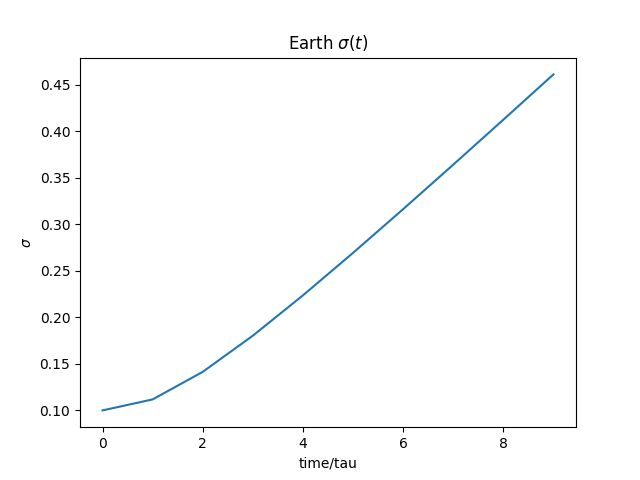
\includegraphics{images2/Earth/sigma.png}
    \caption{Function $\sigma(t)$ for the Earth experiment}
    \label{fig:sigma_earth}
\end{figure}

\begin{figure}[H]
    \centering
     \animategraphics[autoplay, loop]{4}%frame rate
    {images2/Earth/P-}%path to figures
    {0}%start index
    {19}%end index
    \caption{Gif for P(x,t) of the Earth experiment}
    \label{P_earth}
\end{figure}

\textbf{Electron problem: } We want to measure the position of an electron. Our data for this problem is:

\begin{itemize}
    \item $m = 9.11 \cdot 10^{-31} kg$
    \item $ \sigma_0 = 10\% $
    \item $\hbar = 1.05 \cdot 10^{-34} J/s$
\end{itemize}

We want to know the characteristic time first.

\begin{equation}
    \label{2.39}
    \tau = \frac{9.11\cdot 10^{-31}\cdot 0.1^2}{1.05 \cdot 10^{-34}} = 86.76 s 
\end{equation}

We can plot now in steps of $\tau$ the function $\sigma(t)$.

\begin{figure}[H]
    \centering
    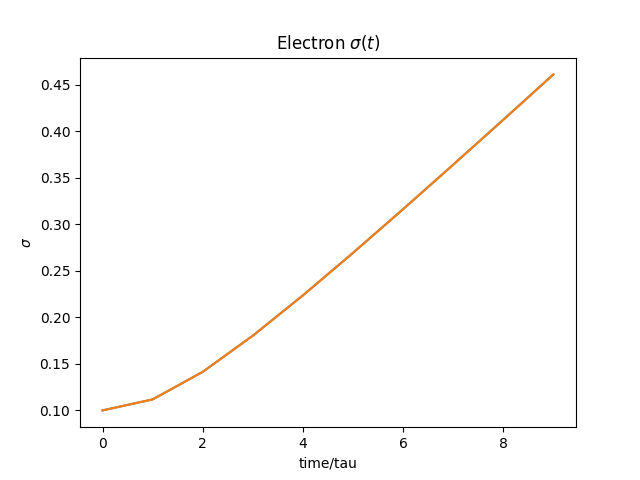
\includegraphics{images2/Electron/sigma.png}
    \caption{Function $\sigma(t)$ for the Electron experiment}
    \label{fig:sigma_electron}
\end{figure}

\begin{figure}[H]
    \centering
     \animategraphics[autoplay, loop]{4}%frame rate
    {images2/Electron/P-}%path to figures
    {0}%start index
    {19}%end index
    \caption{Gif for P(x,t) of the Electron experiment}
    \label{P_electron}
\end{figure}

At a first view the figures for the Earth and the Electron seems similar but we have to think that we are using the characteristic time as a step so the scale is completely different, while the electron functions evolve significantly in less than 100 seconds, the Earth function is changing in an order of $10^{56}$ seconds (MORE THAN THE AGE OF THE UNIVERSE!!). 


\textbf{Neutron problem: } In this experiment we are going to measure the position of a neutron before it decays. A neutron has an average life time of 879 seconds. In this case because we know the scale of time we want to work with we won't calculate the characteristic time now. The data for this experiment is:


\begin{itemize}
    \item $m = 1.67 \cdot 10^{-27} kg$
    \item $ \sigma_0 = 10\% $
    \item $\hbar = 1.05 \cdot 10^{-34} J/s$
\end{itemize}

\begin{figure}[H]
    \centering
    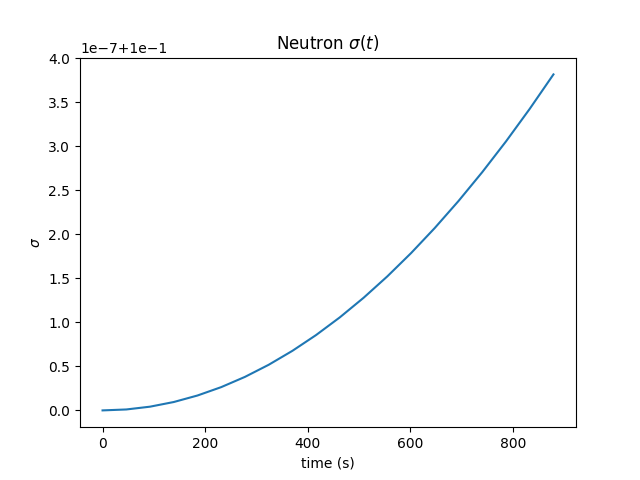
\includegraphics{images2/Neutron/sigma.png}
    \caption{Function $\sigma(t)$ for the Neutron decay}
    \label{fig:sigma_neutron}
\end{figure}

\begin{figure}[H]
    \centering
     \animategraphics[autoplay, loop]{4}%frame rate
    {images2/Neutron/P-}%path to figures
    {0}%start index
    {19}%end index
    \caption{Gif for P(x,t) of the Neutron decay}
    \label{P_neutron}
\end{figure}

In this case we can not appreciate a change in this scale of time. The neutron decays to fast to get an important change in his intensity. But how fast, is to fast? We can calculate the characteristic time to answer this question.

\begin{equation}
    \tau = \frac{1.67 \cdot 10^{-27} 0.1^2}{1.05 \cdot 10^{-34}} = 1.59 \cdot 10^5 s
\end{equation}

We can appreciate in this equation that the characteristic time is almost $10^3$ times bigger than the decay time, that is why we don't get to see a change in the density function among time.

\textbf{Extra problem: } We want to do one more experiment. We can use this functions to know how much it would change the measure of a human. The data is:

\begin{itemize}
    \item $m = 70 kg$
    \item $ \sigma_0 = 10\% $
    \item $\hbar = 1.05 \cdot 10^{-34} J/s$
\end{itemize}

We want to know the characteristic time first.

\begin{equation}
    \label{2.39}
    \tau = \frac{70\cdot 0.1^2}{1.05 \cdot 10^{-34}} = 6.67 \cdot 10^{33} s 
\end{equation}

We can plot now in steps of $\tau$ the function $\sigma(t)$.

\begin{figure}[H]
    \centering
    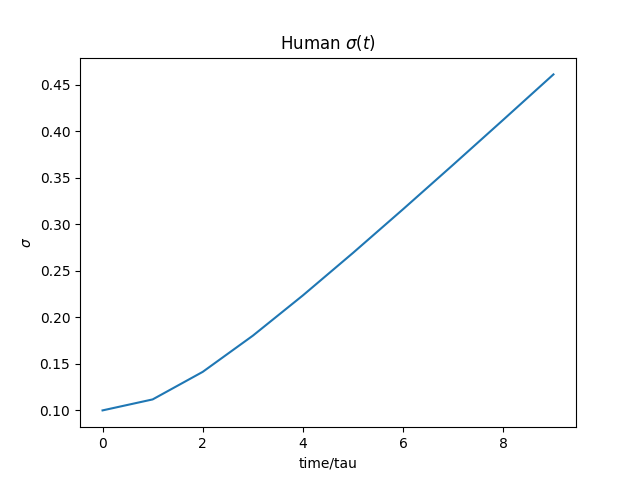
\includegraphics{images2/Human/sigma.png}
    \caption{Function $\sigma(t)$ for the Electron experiment}
    \label{fig:sigma_human}
\end{figure}

\begin{figure}[H]
    \centering
     \animategraphics[autoplay, loop]{4}%frame rate
    {images2/Human/P-}%path to figures
    {0}%start index
    {19}%end index
    \caption{Gif for P(x,t) of the Electron experiment}
    \label{P_human}
\end{figure}


Again we get something similar to the Earth and the Electron problems, but this time our step is an order of $10^{33} s$, this is still larger than the age of the universe.


A free particle is an easy example but we will start with something more difficult in the next chapter.



% In this chapter I will describe the most common options used, both the 
% ones inherited from \Class{scrbook} and the \Class{kao}-specific ones. 
% Options passed to the class modifies its default behaviour; beware 
% though that some options may lead to unexpected results\ldots

% \section{\Class{KOMA} Options}

% The \Class{kaobook} class is based on \Class{scrbook}, therefore it 
% understands all of the options you would normally pass to that class. If 
% you have a lot of patience, you can read the \KOMAScript\xspace 
% guide.\sidenote{The guide can be downloaded from 
% \url{https://ctan.org/pkg/koma-script?lang=en}.} Actually, the reading 
% of such guide is suggested as it is very instructive.

% Every \KOMAScript\xspace option you pass to the class when you load it 
% is automatically activated. In addition, in \Class{kaobook} some options 
% have modified default values. For instance, the font size is 9.5pt and 
% the paragraphs are separated by space,\sidenote[][-7mm]{To be precise, 
% they are separated by half a line worth of space: the \Option{parskip} 
% value is \enquote{half}.} not marked by indentation.

% \section{\Class{kao} Options}

% In the future I plan to add more options to set the paragraph formatting 
% (justified or ragged) and the position of the margins (inner or outer in 
% twoside mode, left or right in oneside mode).\sidenote{As of now, 
% paragraphs are justified, formatted with \Command{singlespacing} (from 
% the \Package{setspace} package) and \Command{frenchspacing}.}

% I take this opportunity to renew the call for help: everyone is 
% encouraged to add features or reimplement existing ones, and to send me 
% the results. You can find the GitHub repository at 
% \url{https://github.com/fmarotta/kaobook}.

% \begin{kaobox}[frametitle=To Do]
% Implement the \Option{justified} and \Option{margin} options. To be 
% consistent with the \KOMAScript\xspace style, they should accept a 
% simple switch as a parameter, where the simple switch should be 
% \Option{true} or \Option{false}, or one of the other standard values for 
% simple switches supported by \KOMAScript. See the \KOMAScript\xspace 
% documentation for further information.
% \end{kaobox}

% The above box is an example of a \Environment{kaobox}, which will be 
% discussed more thoroughly in \frefch{mathematics}. Throughout the book I 
% shall use these boxes to remarks what still needs to be done.

% \section{Other Things Worth Knowing}

% A bunch of packages are already loaded in the class because they are 
% needed for the implementation. These include:

% \begin{itemize}
% 	\item etoolbox
% 	\item calc
% 	\item xifthen
% 	\item xkeyval
% 	\item xparse
% 	\item xstring
% \end{itemize}

% Many more packages are loaded, but they will be discussed in due time. 
% Here, we will mention only one more set of packages, needed to change 
% the paragraph formatting (recall that in the future there will be 
% options to change this). In particular, the packages we load are:

% \begin{itemize}
% 	\item ragged2e
% 	\item setspace
% 	\item hyphenat
% 	\item microtype
% 	\item needspace
% 	\item xspace
% 	\item xcolor (with options \Option{usenames,dvipsnames})
% \end{itemize}

% Some of the above packages do not concern paragraph formatting, but we 
% nevertheless grouped them with the others. By default, the main text is 
% justified and formatted with singlespacing and frenchspacing; the margin 
% text is the same, except that the font is a bit smaller.

% As a last warning, please be aware that the \Package{cleveref} package 
% is not compatible with \Class{kaobook}. You should use the commands 
% discussed in \refsec{hyprefs} instead.

% \section{Document Structure}

% We provide optional arguments to the \Command{title} and 
% \Command{author} commands so that you can insert short, plain text 
% versions of this fields, which can be used, typically in the half-title 
% or somewhere else in the front matter, through the commands 
% \Command{@plaintitle} and \Command{@plainauthor}, respectively. The PDF 
% properties \Option{pdftitle} and \Option{pdfauthor} are automatically 
% set by hyperref to the plain values if present, otherwise to the normal 
% values.\sidenote[][*-1]{We think that this is an important point so 
% we remark it here. If you compile the document with pdflatex, the PDF 
% metadata will be altered so that they match the plain title and author 
% you have specified; if you did not specify them, the metadata will be 
% set to the normal title and author.}

% There are defined two page layouts, \Option{margin} and \Option{wide}, 
% and two page styles, \Option{plain} and \Option{fancy}. The layout 
% basically concern the width of the margins, while the style refers to 
% headers and footer; these issues will be 
% discussed in \frefch{layout}.\sidenote[][6mm]{For now, suffice it to say that pages with 
% the \Option{margin} layout have wide margins, while with the 
% \Option{wide} layout the margins are absent. In \Option{plain} pages the 
% headers and footer are suppressed, while in \Option{fancy} pages there 
% is a header.} 

% The commands \Command{frontmatter}, \Command{mainmatter}, and 
% \Command{backmatter} have been redefined in order to automatically 
% change page layout and style for these sections of the book. The front 
% matter uses the \Option{margin} layout and the \Option{plain} page 
% style. In the mainmatter the margins are wide and the headings are 
% fancy. In the appendix the style and the layout do not change; however 
% we use \Command{bookmarksetup\{startatroot\}} so that the bookmarks of 
% the chapters are on the root level (without this, they would be under 
% the preceding part). In the backmatter the margins shrink again and we 
% also reset the bookmarks root.



\chapter{Potentials V(x,y,z)}

In this chapter we will find the intensity and the $\psi$ function of a particle under a potential. 

\section{Potential in 3 dimensions}

First, we need to define our energy and our equations in 3D, this equations can be obtained from the second chapter generalizing to 3 dimensions.

\begin{equation}
    \label{3.1}
    \frac{p_x^2+p_y^2+p_z^2}{2m}+V(x,y,z) = E
\end{equation}

\begin{equation}
    \label{3.2}
    \left[ -\frac{\hbar^2}{2m} \left[\frac{\partial^2}{\partial x^2}+\frac{\partial^2}{\partial y^2}+\frac{\partial^2}{\partial z^2}  \right] +V(x,y,z) \right] \psi = i\hbar \frac{\partial}{\partial t}\psi
\end{equation}

Where $\psi$ is a function of space and time, i.e. $\psi = \psi(x,y,z,t)$. Before doing some operations with this equations we want to define a boundary for the intensity function. When we talk about this function in the second chapter we define a boundary in \ref{int_P(x)_def}, we need to do the same but in 3 dimensions. 

\begin{equation}
    \label{3.3}
    \int_{-\infty}^{\infty}\int_{-\infty}^{\infty}\int_{-\infty}^{\infty}P(x,y,z)dxdydz = 1
\end{equation}

For this equation to be satisfied we need to achieve this properties:

\begin{itemize}
    \item $\lim_{x\to\infty}P(x,y,z) = 0$ $\forall y,z$
    \item $\lim_{y\to\infty}P(x,y,z) = 0$ $\forall x,z$ 
    \item $\lim_{z\to\infty}P(x,y,z) = 0$ $\forall x,y$ 
\end{itemize}

The intensity is define as $P(x,y,z,t) = \psi\psi^{\star}$. We have defined the intensity and we can continue now with Equation \ref{3.2}. To resolve this we will use the equation and it's conjugate and we will multiply for $\psi$ or $\psi^{\star}$. 

\begin{equation}
    \label{3.4}
    \begin{split}
        &\psi^{\star}\left[ -\frac{\hbar^2}{2m} \left[\frac{\partial^2}{\partial x^2}+\frac{\partial^2}{\partial y^2}+\frac{\partial^2}{\partial z^2}  \right] +V\right] \psi = i \psi^{\star}\hbar \frac{\partial}{\partial t}\psi
        \\
        &\psi\left[ -\frac{\hbar^2}{2m} \left[\frac{\partial^2}{\partial x^2}+\frac{\partial^2}{\partial y^2}+\frac{\partial^2}{\partial z^2}  \right] +V\right] \psi^{\star} = -i \psi \hbar \frac{\partial}{\partial t}\psi^{\star}
    \end{split}
\end{equation}

To continue we will subtract the first equation with the second one.

\begin{equation}
    \label{3.5}
    \begin{split}
        &\frac{\hbar^2}{2m}\left[ \psi \left[ \frac{\partial^2}{\partial x^2}+\frac{\partial^2}{\partial y^2}+\frac{\partial^2}{\partial z^2}\right]\psi^{\star} -\psi^{\star}\left[ \frac{\partial^2}{\partial x^2}+\frac{\partial^2}{\partial y^2}+\frac{\partial^2}{\partial z^2}\right]\psi\right] = i\hbar\left[\psi\frac{\partial}{\partial t}\psi^{\star}+\psi^{\star}\frac{\partial}{\partial t}\psi \right]
        \\
        &\frac{\hbar^2}{2m}\left[\frac{\partial}{\partial x}\left(\psi\frac{\partial}{\partial x}\psi^{\star}-\psi^{\star}\frac{\partial}{\partial x}\psi \right)+\frac{\partial}{\partial y}\left(\psi\frac{\partial}{\partial y}\psi^{\star}-\psi^{\star}\frac{\partial}{\partial y}\psi \right)+
        \\
        &+\frac{\partial}{\partial z}\left(\psi\frac{\partial}{\partial z}\psi^{\star}-\psi^{\star}\frac{\partial}{\partial z}\psi \right) \right] = i\hbar\left[\psi\frac{\partial}{\partial t}\psi^{\star}+\psi^{\star}\frac{\partial}{\partial t}\psi \right]
    \end{split}
\end{equation}

If we integrate both sides we get that the left side is 0.

\begin{equation}
    \label{3.6}
    \begin{split}
    &i\hbar \int_{-\infty}^{\infty}dx\int_{-\infty}^{\infty}dy\int_{-\infty}^{\infty}dz \left[\psi\frac{\partial}{\partial t}\psi^{\star}+\psi^{\star}\frac{\partial}{\partial t}\psi \right] = 0
    \\
    &\frac{d}{dt}\int_{-\infty}^{\infty}dx\int_{-\infty}^{\infty}dy\int_{-\infty}^{\infty}dz \psi \psi^{\star} = 0
    \end{split}
\end{equation}

This equation tell us that the total intensity must be constant among the time, so now we know the conditions of the intensity for space from \ref{3.3} and for time.

\section{Discontinuous Functions}

We will work in one dimension only for now on to get things easier. Some potentials are discontinuous function, one of the most common example is the square well potential. We want to study this discontinuous functions and for that we will recover the delta function.

\begin{marginfigure}
    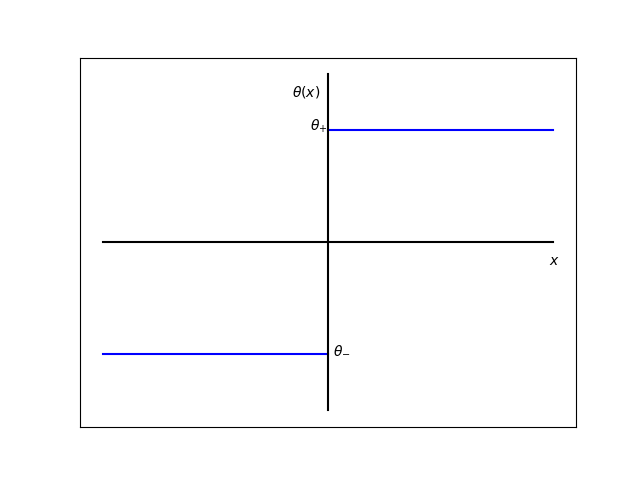
\includegraphics{images3/theta_func.png}
    \caption{Discontinuous function with a finite jump in x = 0}
    \label{theta_func}
\end{marginfigure}


We want to prove that: 

\begin{equation}
    \label{3.7}
    \frac{d\theta}{dx} = C \delta(x)
\end{equation}

This equation is true if: 

\begin{equation}
    \label{3.8}
    \int_{-\infty}^{\infty}f(x) \frac{d\theta}{dx} dx = f(0) C
\end{equation}

Because of the definition of the delta function. To prove this and also to get the value of C we need to operate carefully this integral.

\begin{equation}
    \label{3.9}
    \begin{split}
        &\int_{-\infty}^{\infty}\left( \frac{d}{dx}[f(x)\theta(x)]-\theta(x)\frac{df}{dx}\right)dx = 
        \\
        & = \left[ f(x) \theta(x) \right]_{-\infty}^{\infty}-\int_{-\infty}^{\infty}\frac{d\theta}{dx}\theta(x)dx =
        \\
        & = f(\infty)\theta_+ + f(-\infty)\theta_- + \theta_- \int_{-\infty}^{0}\frac{df}{dx}dx - \theta_+ \int_{0}^{\infty}\frac{df}{dx}dx = 
        \\
        & = f(\infty)\theta_+ + f(-\infty)\theta_- + \theta_- (f(0)-f(-\infty)) - \theta_+ (f(\infty)-f(0))=
        \\
        & = f(0) [\theta_- + \theta_+]
    \end{split}
\end{equation}

We prove that \ref{3.7} is true and also that C is the "jump" distance in the discontinuous function.

%%%%%% CONTINUE THIS PART LATER I DONT UNDERSTAND %%%%%%%%%%%


\section{Square Potential Well}

\begin{figure}[H]
    \centering
    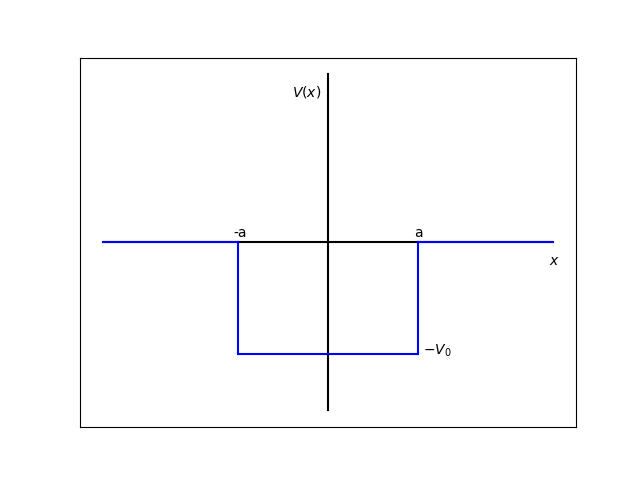
\includegraphics{images3/square_potential.png}
    \caption{Square Potential Well }
    \labfig{fig:square_potential}
\end{figure}

We have a potential as the one in \reffig{fig:square_potential} and we want to study the intensity and the $\psi$ function of a particle among space and time. First i have to define the potential.


\begin{equation}
    f(x) = \frac{-dV}{dx}
\end{equation}

In particle mechanics the problem will be solved with the equation of the energy.

\begin{equation}
    \label{3.11}
    E = \frac{1}{2}m\left(\frac{dx}{dt}\right)^2 + V(x) = constant
\end{equation}

In wave mechanics is more complex we will get the Schrödinguer Wave Equation for one dimension.

\begin{equation}
    \label{3.12}
    i\hbar \frac{\partial\psi(x,t)}{\partial t} = \frac{-\hbar^2}{2m}\frac{\partial^2\psi(x,t)}{\partial x^2} + V(x)\psi(x,t)
\end{equation}

Let's consider one solution to this equation.

\begin{equation}
    \label{3.13}
    \psi(x,t) = \phi(x)e^{-i\frac{E}{\hbar}t}
\end{equation}

Where $\phi(x)$ is a real function, if we remember we solved $\phi(x)$ for the free particle problem and it was a exponential.

\begin{equation}
    \label{3.14}
    \phi(x) = e^{ikx}
\end{equation}

This function does not fulfill equation \ref{3.3}.

\begin{equation}
    \label{3.15}
    \int_{-\infty}^{\infty} \phi^{\star}(x)\phi(x) dx = \infty
\end{equation}

This means that we only have solutions if $V(x) \neq 0$. 

Using our knowledge on the previous section we can get an expression for f(x).

\begin{equation}
    \label{3.16}
    f(x) = \frac{-dV}{dx} = - [ (-V_0-0)\delta(-a) + (0-(-V_0))\delta(a) ] = V_0\delta(-a)-V_0\delta(a)
\end{equation}

We want to redefine the energy, so we do not get stuck with the signs.

Energy = - E where E > 0

For a bound state $0<E<V_0$ must be true. This is a bound state because is similar to the first chapter example when we said that a negative energy implies a closed orbit because the particle must be between the $r_{min}$ and the $r_{max}$ for the energy to be constant, this is exactly the same, but because is in one dimension the particle should bounce between the potential well in a classical approach.

We need now to rewrite the wave equation and the solution.

\begin{equation}
    \psi(x,t) = \phi(x)e^{i\frac{E}{\hbar}t}
\end{equation}

\begin{equation}
    - E\phi(x) = \frac{-\hbar^2}{2m} \frac{d^2\phi(x)}{dx^2}+V(x)\phi(x)
\end{equation}

So the equation for the three different parts of the potential are:

\begin{equation}
    \label{3.19}
    \begin{split}
        & \frac{d^2\phi}{dx^2} = \frac{2mE}{\hbar^2}\phi \hspace{40pt} where \hspace{2pt} x < -a
        \\ 
        & \frac{d^2\phi}{dx^2} = - \frac{2m(V_0-E)}{\hbar^2}\phi \hspace{5pt} where \hspace{2pt} -a < x < a
        \\
        & \frac{d^2\phi}{dx^2} = \frac{2mE}{\hbar^2}\phi \hspace{40pt} where \hspace{2pt} x > a
    \end{split}
\end{equation}

We need to resolve this equations. The solution to this equations are exponential for the first and the third intervals and an addition of a sine and a cosine function.

For the exponential functions we are going to define the exponent as $\alpha$. Because the differential ecuation implies a second derivative this means that the exponential can be $-\alpha$ or $+\alpha$, this sign is going to depend on the equation \ref{3.3}. We are also going to define $\beta$ as the argument of the sine and cosine functions.

\begin{equation}
    \label{3.20}
    \begin{split}
        & \alpha = a\sqrt{\frac{2mE}{\hbar^2}}
        \\
        & \beta = a \sqrt{\frac{2m(V_0-E)}{\hbar^2}}
        \\
        & \gamma^2 = \beta^2 + \alpha^2 = a^2\frac{2mV_0}{\hbar^2} 
    \end{split}
\end{equation}

We have also defined gamma, that is a constant of the problem (does not depend on the energy) and is going to be useful to determine the values of $\alpha$ and $\beta$ after we solve the equations.

We can solve now our differential equations.

\begin{equation}
    \label{3.21}
    \begin{split}
                    & Ae^{\frac{-\alpha}{a}x} \hspace{90pt} x > a
                    \\
       \psi(x) =    & B \sin{(\frac{\beta}{a}x)} + C \cos{(\frac{\beta}{a}x)} \hspace{10pt} -a < x < a 
                    \\
                    & De^{\frac{\alpha}{a}x} \hspace{90pt} x < -a
    \end{split}
\end{equation}

Now we need to use the boundary conditions. We already know that \ref{3.3} must be true and we will use that condition later, but we also know that $\phi$ must be continuous because we define it as a continuous function and the first derivative must be continuous also because if not, then we will have Dirac's delta functions in the wave equation that can not cancel with anything. So we have two boundary conditions that will became 4 equations. But before we will do some changes in \ref{3.21} to get easier equations later.

\begin{equation}
    \label{3.22}
    \begin{split}
                    & Ae^{\frac{-\alpha}{a}x} \hspace{120pt} x > a
                    \\
       \psi(x) =    & B\textcolor{red}{e^{-\alpha}} \sin{(\frac{\beta}{a}x)} + C\textcolor{red}{e^{-\alpha}} \cos{(\frac{\beta}{a}x)} \hspace{10pt} -a < x < a 
                    \\
                    & De^{\frac{\alpha}{a}x} \hspace{120pt} x < -a
    \end{split}
\end{equation}



The continuity conditions can be set now.

\begin{equation}
    \label{3.23}
    \begin{split}
        &  D = -B sin(\beta) + C cos(\beta)
        \\
        & A = B sin(\beta) + C cos(\beta)
        \\
        & D\alpha = B\beta cos(\beta) + C \beta sin(\beta)
        \\
        & -A \alpha = B\beta cos(\beta)-C \beta sin(\beta)
    \end{split}
\end{equation}

This is a homogeneous system, so one of the solutions is A=B=C=D=0 but this solution is not allowed. If we solved for this we will get two equations that actually imply 4 equations.

\begin{equation}
\label{3.24}
\begin{split}
    & C (\alpha cos(\beta)-\beta sin(\beta)) = 0
    \\
    & B (\alpha sin(\beta)+\beta cos(\beta)) = 0
\end{split}
\end{equation}

If B = C = 0, A and D will be 0 also and we already said that is not an option, so we have three possibilities. Let's try doing both parenthesis equal to 0 and add them multiplying by some factor.

\begin{equation}
\begin{split}
        &
        sin(\beta)(\alpha sin(\beta) + \beta cos(\beta)) + cos(\beta)(\alpha cos(\beta) - \beta sin(\beta)) = 0 \\
        & \alpha sin^2(\beta) + \alpha cos^2(\beta) = 0
\end{split}
\end{equation}

With our choice the solution is $\alpha = 0$ but $\alpha$ can not be 0, so we only have two choices both of them are right.


If we take a look at this dependency between $\alpha$ and $\beta$ and we include our gamma equation to the chart we would see something interesting.

\begin{equation}
    \begin{split}
        & \alpha = -\beta \cot{(\beta)}
        \\
        & \alpha = \beta \tan{(\beta)}
        \\
        & \gamma^2 = \alpha^2 + \beta^2
    \end{split}
\end{equation}

\begin{figure}[H]
    \centering
    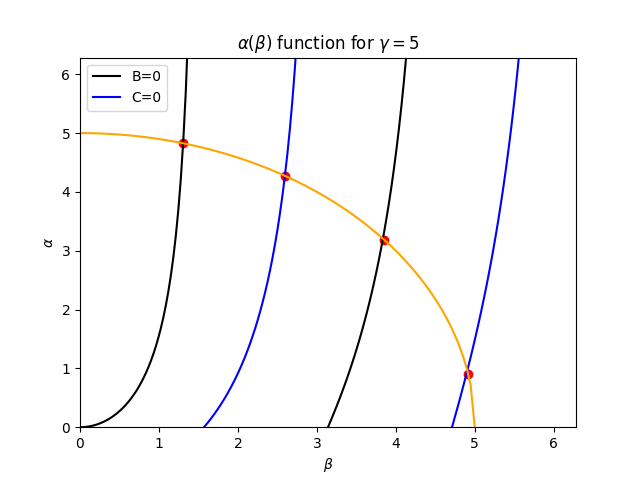
\includegraphics{images3/alpha_beta.png}
    \caption{$\alpha$ as a function of $\beta$ for $\gamma = 5$}
    \labfig{alpha_beta}
\end{figure}

This proves that the energy is quantized because only some values for $\alpha$ (that is a function of Energy) are possible.

And the solutions are:

Solution for C = 0
\begin{equation}
     \begin{split}
        & A = B sin(\beta)
        \\
        & B = B
        \\
        & C = 0
        \\
        & D = - B sin(\beta)
     \end{split}
\end{equation}

Solution for B = 0
\begin{equation}
     \begin{split}
        & A = C cos(\beta)
        \\
        & B = 0
        \\
        & C = C
        \\
        & D = C cos(\beta)
     \end{split}
\end{equation}



We still have one variable left to resolve, to do this we will need to use \ref{3.3}. We will resolve only for the case B = 0, the other one will turn the same.

\begin{equation}
    \label{3.29}
    \begin{split}
        & \int_{-\infty}^{\infty} \phi^2(x) dx = 
        \\
        & = C^2\left[ cos^2(\beta) \int_{-\infty}^{-a}e^{\frac{2\alpha}{a}x}dx + e^{-2\alpha}\int_{-a}^{a} cos^2(\frac{\beta}{a}x) dx + cos^2(\beta) \int_{a}^{\infty}e^{-\frac{2\alpha}{a}x}dx \right]=
        \\
        & =  C^2\left[ cos^2(\beta)\frac{a}{2\alpha} \left[e^{\frac{2\alpha}{a}x}\right]_{-\infty}^{-a} 
        + \frac{e^{-2\alpha}}{2} \left[\frac{a}{2\beta}sin(\frac{2\beta}{a}x)+x\right]_{-a}^{a} 
        - cos^2(\beta) \frac{a}{2\alpha} \left[e^{\frac{2\alpha}{a}x}\right]_{a}^{\infty} \right] =
        \\
        & C^2 a e^{-2\alpha}\left[\frac{cos^2(\beta)}{\beta\tan{(\beta)}}+\frac{sin(2\beta)}{2\beta}+1\right] =
        \\
        & = C^2ae^{-2\alpha}\left[\frac{1}{\alpha}+1\right] = 1
    \end{split}
\end{equation}

Now we need to resolve for C in the last step.

\begin{equation}
    \label{3.30}
    C^2 = \frac{\alpha e^{2\alpha}}{a(1+\alpha)}
\end{equation}

If C=0 then, $B^2$ is equal to the expression above. 

Now we can solve for everything in the problem for a given gamma.


\section{Examples}

We will plot some of the solutions for different gamma and for the largest gamma we will try to approach and explain a classical behaviour.

\textbf{First example: } In this case we will took gamma = 10, and plot two of the solutions, one for B=0 and the other one for C=0.

\begin{figure}[H]
    \centering
    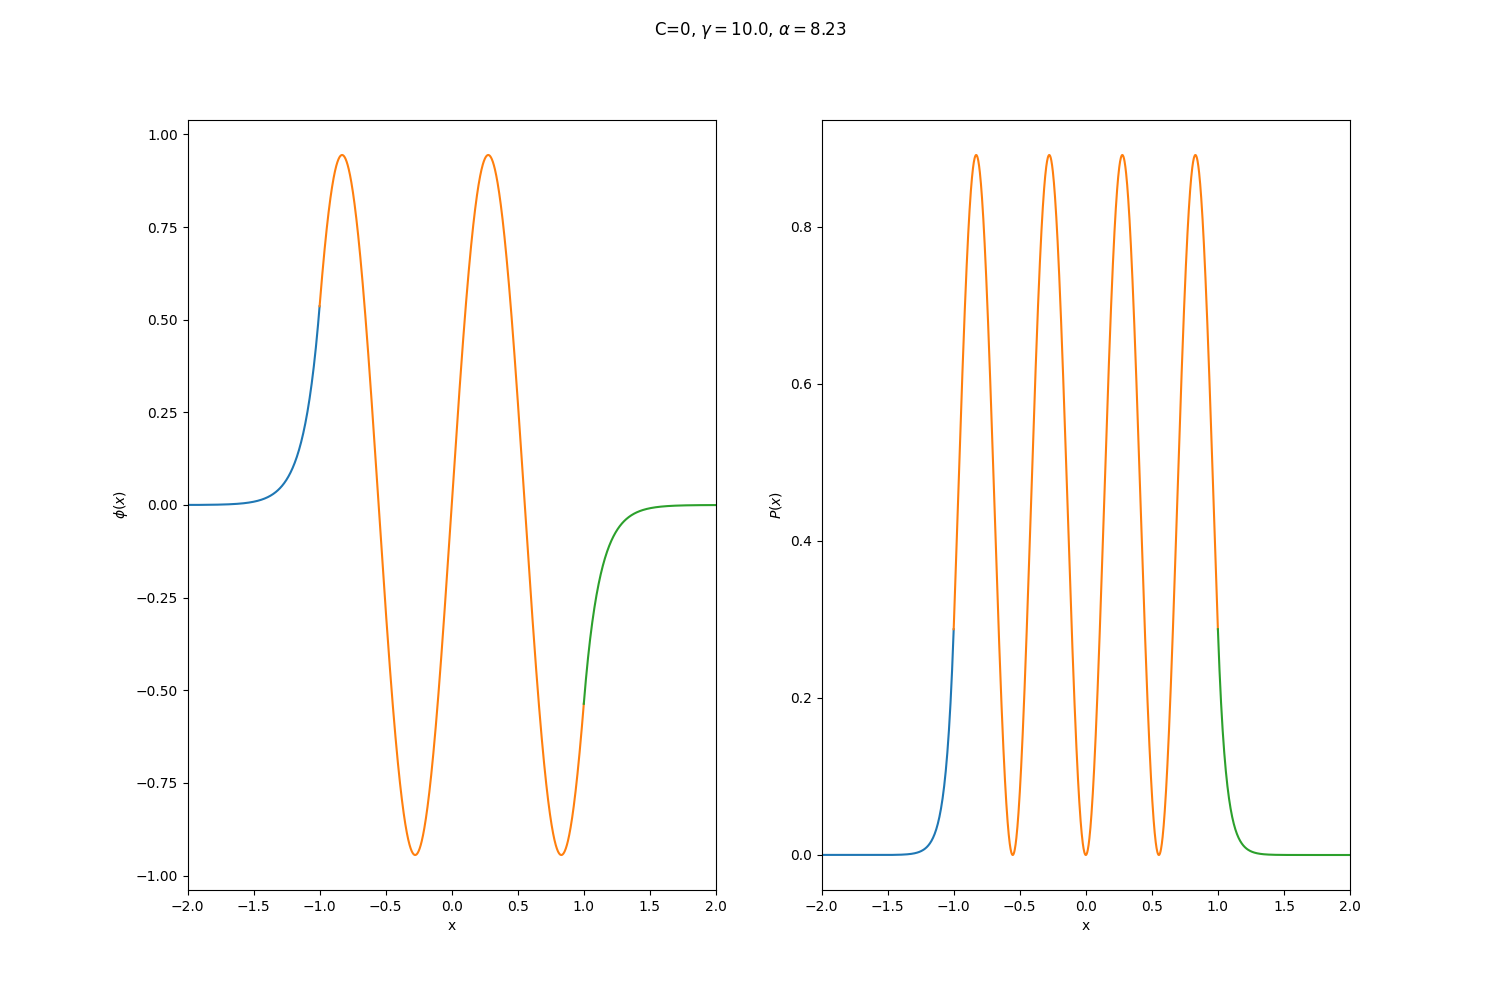
\includegraphics{images3/phi_gamma=10.0_alpha=8.23.png}
    \caption{$\phi(x)$ and P(x) functions for gamma = 10}
    \label{gamma1=10}
\end{figure}

\begin{figure}[H]
    \centering
    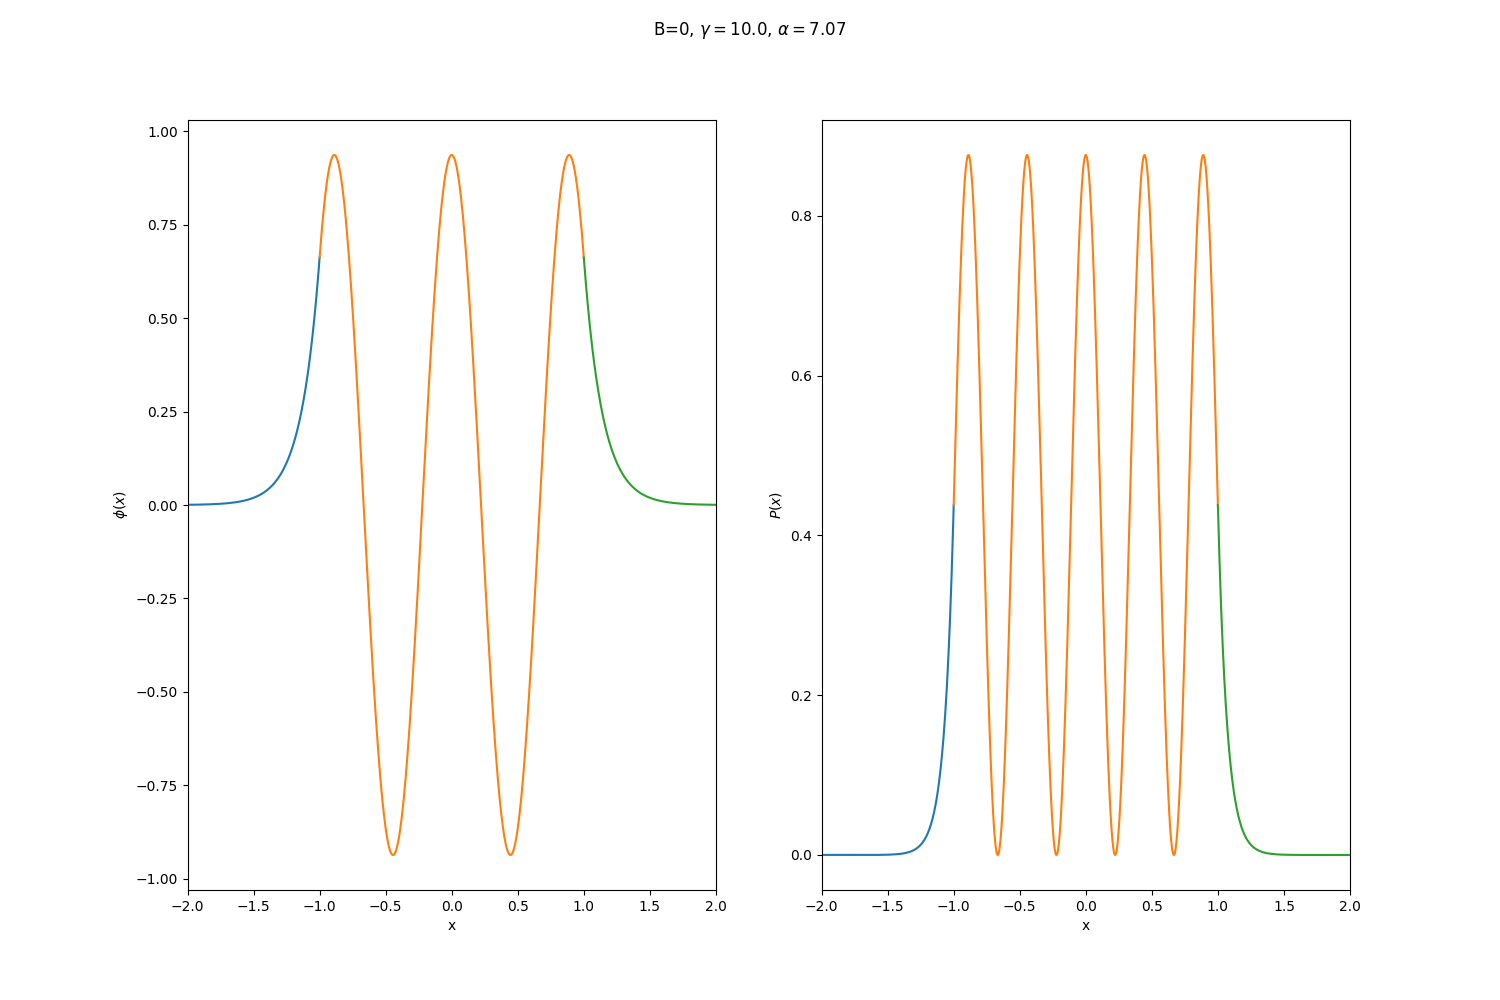
\includegraphics{images3/phi_gamma=10.0_alpha=7.07.png}
    \caption{$\phi(x)$ and P(x) functions for gamma = 10}
    \label{gamma2=10}
\end{figure}

Now we will try to achieve a similar behaviour to the well-known particle approach, where all the probability is inside the square root potential and all of it is equally likely to have the particle. We can achieve this finding the P(x) function for a bigger gamma and a small alpha.

\begin{figure}[H]
    \centering
    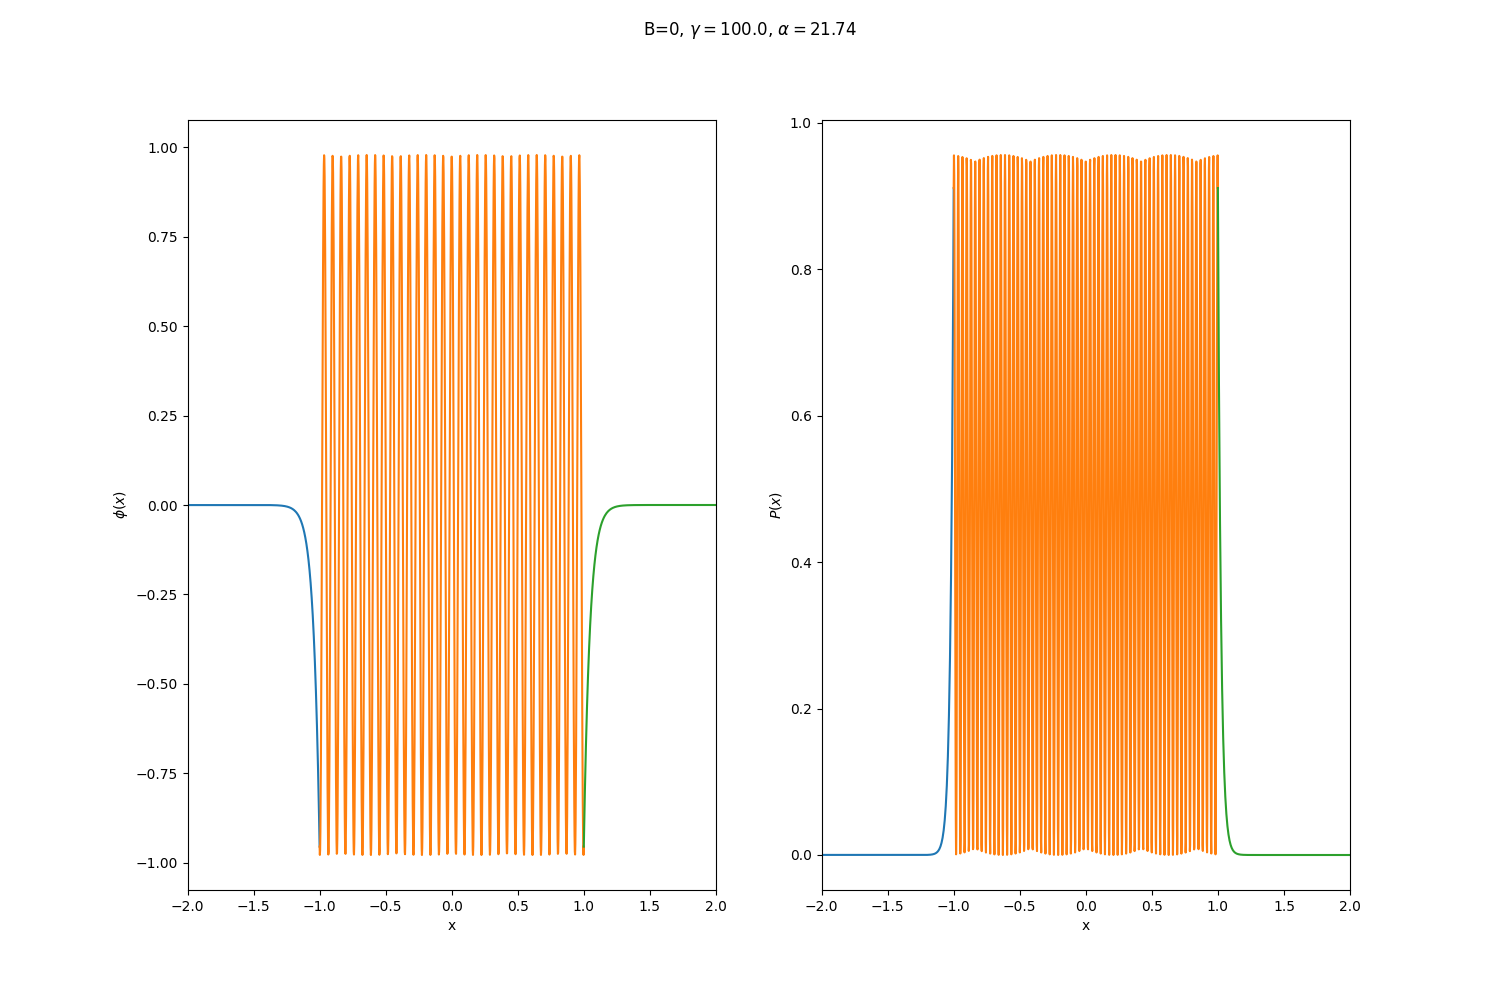
\includegraphics{images3/phi_gamma=100.0_alpha=21.74.png}
    \caption{$\phi(x)$ and P(x) functions for gamma = 100}
    \labfig{gamma=100}
\end{figure}

In \reffig{gamma=100} we can see that we get what we expect for a particle behaviour but we still have that quantum behaviour because the integral outside of the square potential is not zero as it should be in the particle behaviour.


% \setchapterimage[7.5cm]{seaside}
% \setchapterpreamble[u]{\margintoc}
% %\chapter[Figures and Tables]{Figures and Tables\footnotemark[0]}
% \chapter{Figures and Tables}

% \footnotetext{The credits for the image above the chapter title go to:
% 	Bushra Feroz, CC~BY-SA~4.0, \url{https://commons.wikimedia.org/w/index.php?curid=68724647}}

% \section{Normal Figures and Tables}

% Figures and tables can be inserted just like in any standard 
% \LaTeX\xspace document. The \Package{graphicx} package is already loaded 
% and configured in such a way that the figure width is equal to the 
% textwidth and the height is adjusted in order to maintain the original 
% aspect ratio. As you may have imagined, the captions will be 
% positioned\ldots well, in the margins. This is achieved with the help of 
% the \Package{floatrow} package.

% Here is a picture of Mona Lisa (\reffig{normalmonalisa}), as an example. 
% The captions are formatted as the margin- and the side-notes; If you 
% want to change something about captions you can use the command 
% \Command{captsetup} from the \Package{caption} package. Remember that if 
% you want to reference a figure, the label must come \emph{after} the 
% caption!

% \begin{figure}[hb]
% 	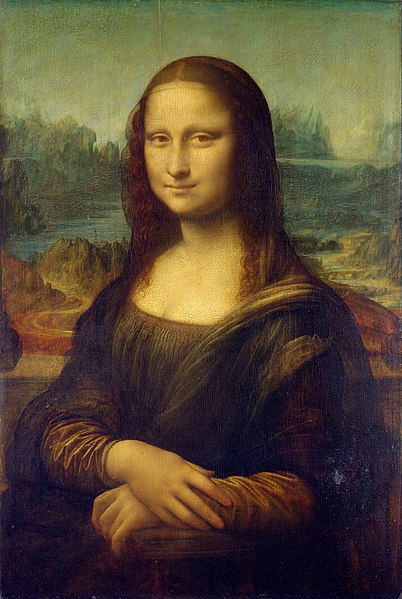
\includegraphics[width=0.45\textwidth]{monalisa}
% 	\caption[Mona Lisa, again]{It's Mona Lisa again. \blindtext}
% 	\labfig{normalmonalisa}
% \end{figure}

% While the format of the caption is managed by \Package{caption}, its 
% position is handled by the \Package{floatrow} package. Achieving this 
% result has been quite hard, but now I am pretty satisfied. In two-side 
% mode, the captions are printed in the correct margin.

% Tables can be inserted just as easily as figures, as exemplified by the 
% following code:

% \begin{lstlisting}[caption={Caption of a listing.}]
% \begin{table}
% \begin{tabular}{ c c c c }
% 	\toprule
% 	col1 & col2 & col3 & col 4 \\
% 	\midrule
% 	\multirow{3}{4em}{Multiple row} & cell2 & cell3 & cell4\\ &
% 	cell5 & cell6 & cell7 \\ &
% 	cell8 & cell9 & cell10 \\
% 	\multirow{3}{4em}{Multiple row} & cell2 & cell3 & cell4 \\ &
% 	cell5 & cell6 & cell7 \\ &
% 	cell8 & cell9 & cell10 \\
% 	\bottomrule
% \end{tabular}
% \end{table}
% \end{lstlisting}

% which results in the useless \vreftab{useless}.

% \begin{table}[ht]
% \caption[A useless table]{A useless table.}
% \labtab{useless}
% \begin{tabular}{ c c c c }
% 	\toprule
% 	col1 & col2 & col3 & col 4 \\
% 	\midrule
% 	\multirow{3}{4em}{Multiple row} & cell2 & cell3 & cell4\\ &
% 	cell5 & cell6 & cell7 \\ &
% 	cell8 & cell9 & cell10 \\
% 	\multirow{3}{4em}{Multiple row} & cell2 & cell3 & cell4 \\ &
% 	cell5 & cell6 & cell7 \\ &
% 	cell8 & cell9 & cell10 \\
% 	\bottomrule
% \end{tabular}
% \end{table}

% I don't have much else to say, so I will just insert some blind text. 
% \blindtext

% \section{Margin Figures and Tables}

% Marginfigures can be inserted with the environment 
% \Environment{marginfigure}. In this case, the whole picture is confined 
% to the margin and the caption is below it. \reffig{marginmonalisa} is 
% obtained with something like this:

% \begin{lstlisting}[caption={Another caption.}]
% \begin{marginfigure}
% 	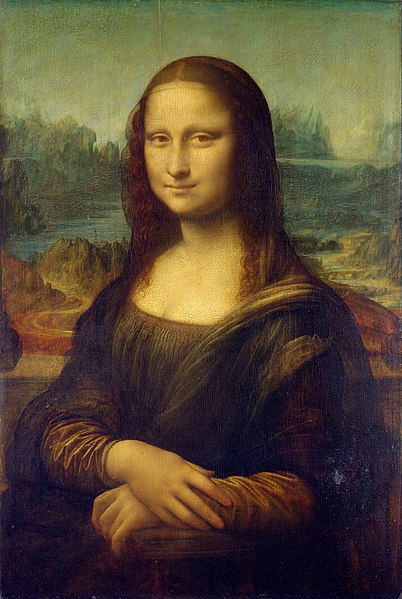
\includegraphics{monalisa}
% 	\caption[The Mona Lisa]{The Mona Lisa.}
% 	\labfig{marginmonalisa}
% \end{marginfigure}
% \end{lstlisting}

% There is also the \Environment{margintable} environment, of which 
% \reftab{anotheruseless} is an example. Notice how you can place the 
% caption above the table by just placing the \Command{caption} command 
% before beginning the \Environment{tabular} environment. Usually, figure 
% captions are below, while table captions are above. This rule is also 
% respected for normal figures and tables: the captions are always on the 
% side, but for figure they are aligned to the bottom, while for tables to 
% the top.

% \begin{margintable}
% \caption[Another useless table]{Another useless table.}
% \labtab{anotheruseless}
% \raggedright
% \begin{tabular}{ c c c c }
% 	\hline
% 	col1 & col2 & col3 \\
% 	\hline
% 	\multirow{3}{4em}{Multiple row} & cell2 & cell3 \\ & cell5 & cell6 
% 	\\ & cell8 & cell9 \\ \hline
% \end{tabular}
% \end{margintable}

% Marginfigures and tables can be positioned with an optional offset 
% command, like so:

% \begin{lstlisting}
% \begin{marginfigure}[offset]
% 	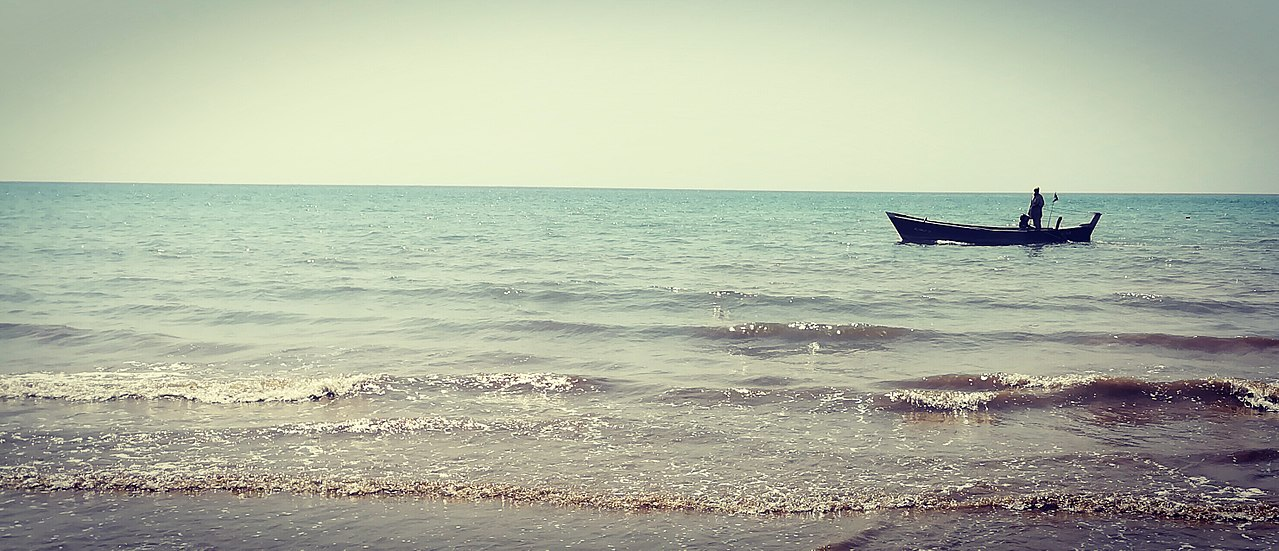
\includegraphics{seaside}
% \end{marginfigure}
% \end{lstlisting}

% Offset ca be either a measure or a multiple of \Command{baselineskip}, 
% much like with \Command{sidenote}, \Command{marginnote} and 
% \Command{margintoc}.\todo{Improve this part.} If you are wondering how I 
% inserted this orange bubble, have a look at the \Package{todo} package.

% \section{Wide Figures and Tables}

% With the environments \Environment{figure*} and \Environment{table*} you 
% can insert figures which span the whole page width. For example, here 
% are a wide figure and a wide table.

% \begin{figure*}[h!]
% 	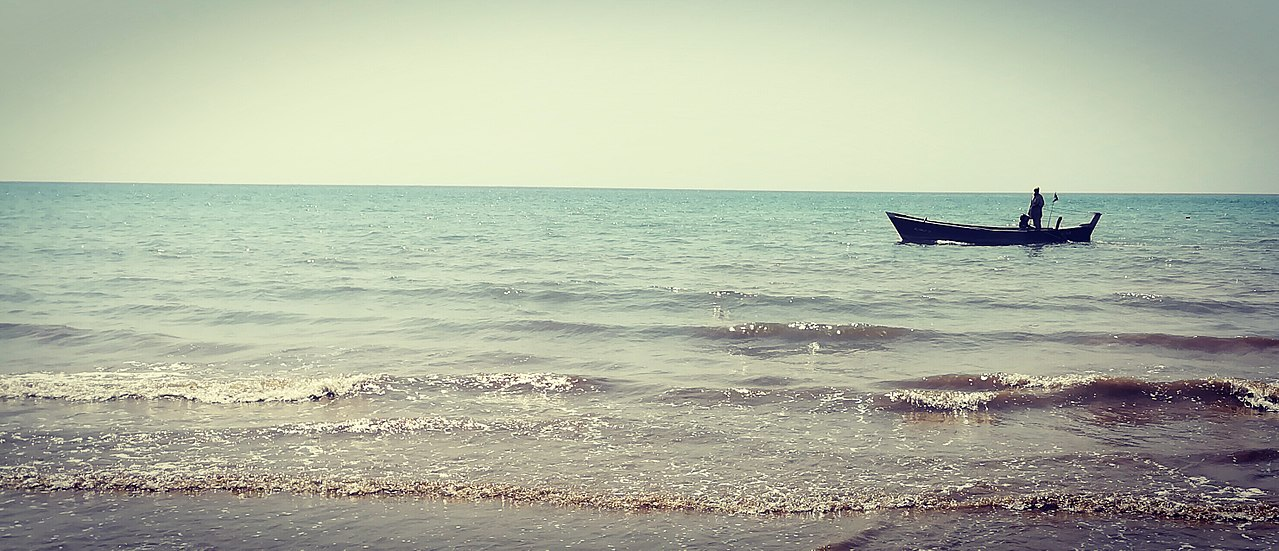
\includegraphics{seaside}
% 	\caption[A wide seaside]{A wide seaside, and a wide caption.
% 		Credits: By Bushra Feroz, CC BY-SA 4.0, \url{https://commons.wikimedia.org/w/index.php?curid=68724647}}
% \end{figure*}

% \begin{table*}[h!]
%     \caption{A wide table with invented data about three people living in the UK. Note that wide figures and tables are centered and their caption also extends into the margin.}
%     \begin{tabular}{p{2.0cm} p{2.0cm} p{2.0cm} p{2.0cm} p{2.0cm} p{2.0cm} p{1.5cm}}
%         \toprule
%         Name    & Surname   & Job       & Salary           & Age   & Height    & Country \\
%         \midrule
%         Alice   & Red       & Writer    & 4.000 \pounds    & 34    & 167 cm     & England \\
%         Bob     & White     & Bartender & 2.000 \pounds    & 24    & 180 cm     & Scotland \\
%         Drake   & Green     & Scientist & 4.000 \pounds    & 26    & 175 cm     & Wales \\
%         \bottomrule
%     \end{tabular}
% \end{table*}

% It is the user's responsibility to adjust the width of the table, if 
% necessary, until it is aesthetically pleasing. The previous table was 
% obtained with the following code:

% \begin{lstlisting}[caption=How to typeset a wide table]
% \begin{table*}[h!]
%     \caption{A wide table with invented data about three people living in the UK. Note that wide figures and tables are centered and their caption also extends into the margin.}
%     \begin{tabular}{p{2.0cm} p{2.0cm} p{2.0cm} p{2.0cm} p{2.0cm} p{2.0cm} p{1.5cm}}
%         \toprule
%         Name    & Surname   & Job       & Salary           & Age   & Height    & Country \\
%         \midrule
%         Alice   & Red       & Writer    & 4.000 \pounds    & 34    & 167 cm     & England \\
%         Bob     & White     & Bartender & 2.000 \pounds    & 24    & 180 cm     & Scotland \\
%         Drake   & Green     & Scientist & 4.000 \pounds    & 26    & 175 cm     & Wales \\
%         \bottomrule
%     \end{tabular}
% \end{table*}
% \end{lstlisting}

% The \Package{floatrow} package provides the \enquote{H} specifier to 
% instruct \LaTeX to position the figure (or table) in precisely the same 
% position it occupies in the source code. However, this specifier does 
% not work with wide figures or tables: you should use \enquote{h!} 
% instead, like so: \lstinline|\begin{figure*}[h!]|.

% You may have noticed the full width image at the very beginning of this
% chapter: that, however, is set up in an entirely different way, which
% you'll read about in \vrefch{layout}.

% \Class{kaobook} also supports paginated tables (have a look at the 
% \Package{longtable} package). The 
% \Environment{longtable}\sidenote{Interestingly, \Environment{longtable}s 
% may require up to four rounds of compilation before they are typeset 
% correctly.} environment behaves a bit differently from 
% \Environment{table}, in that \Environment{longtable} encompasses both 
% \Environment{table} and \Environment{tabular}, so that you can write, 
% \eg,

% \begin{lstlisting}[caption=Example of a longtable]
% \begin{longtable}{|l c c|}
%     \hline
%     One & Two & Three \\
%     Left & Center & Center \\
%     \hline
%     \caption{Caption of the longtable.}
% \end{longtable}
% \end{lstlisting}

% to obtain the following table:
% \begin{longtable}{|l c c|}
%     \hline
%     One & Two & Three \\
%     Left & Center & Center \\
%     \hline
%     \caption{Caption of the longtable.}
% \end{longtable}

% The caption of a \Environment{longtable} is always positioned below the 
% table, and it has the same width as the text (it doesn't extend into the 
% margin). However, sometimes you may need a \Environment{longtable} that 
% is so wide that it trespass into the margins; in those cases, you may 
% want to also increase the width of the caption. To do so, you'll have to 
% write two additional commands, one before and one after the 
% \Environment{longtable}:

% \begin{lstlisting}[caption=Increasing the width of the caption of a \Environment{longtable}.]
% \floatsetup[longtable]{margins=centering,LTcapwidth=table} % Add this line before the longtable to increase the caption width
% \begin{longtable}{lp{8cm}p{5cm}p{2cm}}
% ...
% \end{longtable}
% \floatsetup[longtable]{margins=raggedright,LTcapwidth=\textwidth} % Add this line after the longtable to revert the previous change
% \end{lstlisting}

% Having seen figures and tables, it is now time to tackle 
% hyperreferences.


% \setchapterpreamble[u]{\margintoc}
% \chapter{Margin Stuff}

% Sidenotes are a distinctive feature of all 1.5-column-layout books.
% Indeed, having wide margins means that some material can be displayed
% there. We use margins for all kind of stuff: sidenotes, marginnotes,
% small tables of contents, citations, and, why not?, special boxes and
% environments.

% \section{Sidenotes}

% Sidenotes are like footnotes, except that they go in the margin, where
% they are more readable. To insert a sidenote, just use the command
% \Command{sidenote\{Text of the note\}}. You can specify a
% mark\sidenote[O]{This sidenote has a special mark, a big O!} with \\
% \Command{sidenote[mark]\{Text\}}, but you can also specify an offset,
% which moves the sidenote upwards or downwards, so that the full syntax is:

% \begin{lstlisting}[style=kaolstplain]
% \sidenote[mark][offset]{Text}
% \end{lstlisting}

% If you use an offset, you always have to add the brackets for the mark,
% but they can be empty.\sidenote{If you want to know more about the usage
% of the \Command{sidenote} command, read the documentation of the
% \Package{sidenotes} package.}

% In \Class{kaobook} we copied a feature from the \Package{snotez}
% package: the possibility to specify a multiple of \Command{baselineskip}
% as an offset. For example, if you want to enter a sidenote with the
% normal mark and move it upwards one line, type:

% \begin{lstlisting}[style=kaolstplain]
% \sidenote[][*-1]{Text of the sidenote.}
% \end{lstlisting}

% As we said, sidenotes are handled through the \Package{sidenotes}
% package, which in turn relies on the \Package{marginnote} package.

% \section{Marginnotes}

% This command is very similar to the previous one. You can create a
% marginnote with \Command{marginnote[offset]\{Text\}}, where the offset
% argument can be left out, or it can be a multiple of
% \Command{baselineskip},\marginnote[-1cm]{While the command for margin
% notes comes from the \Package{marginnote} package, it has been redefined
% in order to change the position of the optional offset argument, which
% now precedes the text of the note, whereas in the original version it
% was at the end. We have also added the possibility to use a multiple of
% \Command{baselineskip} as offset. These things were made only to make
% everything more consistent, so that you have to remember less things!}
% \eg

% \begin{lstlisting}[style=kaolstplain]
% \marginnote[-12pt]{Text} or \marginnote[*-3]{Text}
% \end{lstlisting}

% \begin{kaobox}[frametitle=To Do]
% A small thing that needs to be done is to renew the \Command{sidenote}
% command so that it takes only one optional argument, the offset. The
% special mark argument can go somewhere else. In other words, we want the
% syntax of \Command{sidenote} to resemble that of \Command{marginnote}.
% \end{kaobox}

% We load the packages \Package{marginnote}, \Package{marginfix} and
% \Package{placeins}. Since \Package{sidenotes} uses \Package{marginnote},
% what we said for marginnotes is also valid for sidenotes. Side- and
% margin- notes are shifted slightly upwards
% (\Command{renewcommand\{\textbackslash marginnotevadjust\}\{3pt\}}) in
% order to align them to the bottom of the line of text where the note is
% issued. Importantly, both sidenotes and marginnotes are defined as
% floating if the optional argument (\ie the vertical offset) is left
% blank, but if the offset is specified they are not floating. Recall that
% floats cannot be nested, so in some rare cases you may encounter errors
% about lost floats; in those cases, remember that sidenotes and
% marginnotes are floats. To solve the problem, it may be possible to
% transform them into non-floating elements by specifying an offset of
% 0pt.

% \section{Footnotes}

% Even though they are not displayed in the margin, we will discuss about
% footnotes here, since sidenotes are mainly intended to be a replacement
% of them. Footnotes force the reader to constantly move from one area of
% the page to the other. Arguably, marginnotes solve this issue, so you
% should not use footnotes. Nevertheless, for completeness, we have left
% the standard command \Command{footnote}, just in case you want to put a
% footnote once in a while.\footnote{And this is how they look like.
% Notice that in the PDF file there is a back reference to the text;
% pretty cool, uh?}

% \section{Margintoc}

% Since we are talking about margins, we introduce here the
% \Command{margintoc} command, which allows one to put small table of
% contents in the margin. Like other commands we have discussed,
% \Command{margintoc} accepts a parameter for the vertical offset, like
% so: \Command{margintoc[offset]}.

% The command can be used in any point of the document, but we think it
% makes sense to use it just at the beginning of chapters or parts. In
% this document I make use of a \KOMAScript\xspace feature and put it in
% the chapter preamble, with the following code:

% \marginnote{The font used in the margintoc is the same as the one for
% 	the chapter entries in the main table of contents at the beginning
% 	of the document.}

% \begin{lstlisting}[style=kaolstplain]
% \setchapterpreamble[u]{\margintoc}
% \chapter{Chapter title}
% \end{lstlisting}

% As the space in the margin is a valuable resource, there is the
% possibility to print a shorter version of the title in the margin toc.
% Thus, there are in total three possible versions for the title of a
% section (or subsection): the one for the main text, the one for the main
% table of contents, and the one for the margintoc. These versions can be
% specified at the same time when the section is created in the source
% \TeX file:
% \begin{lstlisting}[style=kaolstplain]
% \section[alternative-title-for-toc]{title-as-written-in-text}[alternative-title-for-margintoc]
% \end{lstlisting}

% By default, the margintoc includes sections and subsections.
% If you only want to show sections, add
% \begin{lstlisting}[style=kaolstplain]
% \setcounter{margintocdepth}{\sectiontocdepth}
% \end{lstlisting}
% somewhere in your preamble.

% \section{Marginlisting}

% On some occasions it may happen that you have a very short piece of code
% that doesn't look good in the body of the text because it breaks the
% flow of narration: for that occasions, you can use a
% \Environment{marginlisting}. The support for this feature is still
% limited, especially for the captions, but you can try the following
% code:

% \begin{marginlisting}[-1.35cm]
% 	\caption{An example of a margin listing.}
% 	\vspace{0.6cm}
% 	\begin{lstlisting}[language=Python,style=kaolstplain]
% print("Hello World!")
% 	\end{lstlisting}
% \end{marginlisting}

% \begin{verbatim}
% \begin{marginlisting}[-0.5cm]
% 	\caption{My caption}
% 	\vspace{0.2cm}
% 	\begin{lstlisting}[language=Python,style=kaolstplain]
% 	... code ...
% 	\end{lstlisting}
% \end{marginlisting}
% \end{verbatim}

% Unfortunately, the space between the caption and the listing must be
% adjusted manually; if you find a better way, please let me know.

% Not only textual stuff can be displayed in the margin, but also figures.
% Those will be the focus of the next chapter.

\setchapterpreamble[u]{\margintoc}
\chapter{Delta function potential}

We want to understand solids and their properties, for example why copper is a conductor and wood is not? For this and other questions we will propose our next problem, the delta function potential problem.


\section{Definition of the potential}

We define our potential this time as

\begin{equation}
    \label{4.1}
    V(x) = -2C\delta(x)
\end{equation}

Where $C= V_0a$.

\begin{marginfigure}
  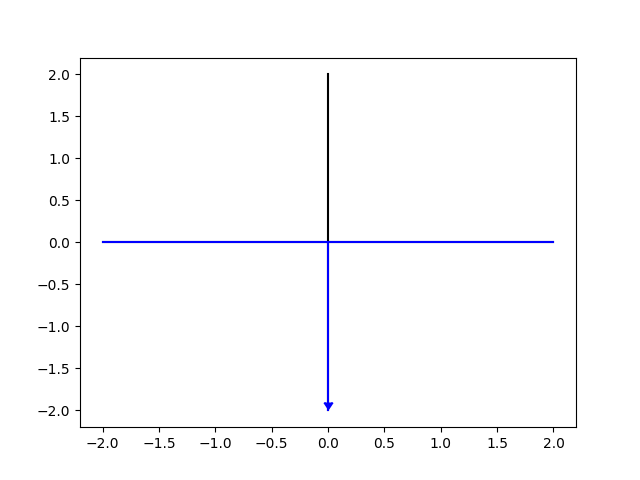
\includegraphics{images4/delta.png}
  \caption{Delta function potential}
  \label{figure4-1}
\end{marginfigure}

Because we have delta functions in our equations we can not call them normal equations so we will use quotes to differentiate them from real equations.

\begin{equation}
    "+\frac{\hbar^2}{2m}\frac{\partial^2\phi}{\partial x^2} + 2C\delta(x) \phi(x) = + E \phi(x)"
\end{equation}

\section{Solution}

The solution for this equation is:

\begin{equation}
    \label{4.3}
    \psi(x,t) = e^{i\frac{E}{\hbar}t} \phi(x)
\end{equation}

Now we need to solve our equation for $\phi(x)$.

\begin{equation}
    \label{4.4}
    \begin{split}
    & "\frac{\partial^2\phi}{\partial x^2}+\frac{4mC}{\hbar^2}\delta(x)\phi(x)= \frac{2mE}{\hbar^2}\phi(x)" \\
    & "\frac{\partial^2\phi}{\partial x^2}+\frac{4mV_0a}{\hbar^2}\delta(x)\phi(x)= \frac{2mE}{\hbar^2}\phi(x)"
    \end{split}
\end{equation}

We need to define two variables to resolve this equations, $\alpha$ and g (This variables are completely different to the variables in the previous chapter).

\begin{equation}
    \label{4.5}
    \begin{split}
    & g = \frac{2mV_0a}{\hbar^2} \\
    & \alpha = \sqrt{\frac{2mE}{\hbar^2}}
    \end{split}
\end{equation}

As we did in the previous chapter we have to think about the continuity in $\phi(x)$. Can $\phi(x)$ be discontinuous? The answer is no. $\phi(x)$ is continuous because if it weren't continues the second derivative would look like the derivative of a delta function and the equations don't make sense with that assumption. However, in this case the first derivative of $\phi(x)$ must be discontinuous because we need the second derivative to go as a delta function.

We solve for $\phi(x) \neq 0$.

\begin{equation}
    \label{4.6}
    \frac{\partial^2\phi(x)}{\partial x^2} = \alpha^2\phi(x)
\end{equation}

The solution to this differential equation is:

\begin{equation}
    \label{4.7}
    \begin{split}
        \phi(x)= \left\{ \begin{array}{lcc} Ae^{\alpha x} & where & x \leq 0 \\
        \\ Ae^{-\alpha x} & where & x \geq 0 \end{array} \right.
    \end{split}
\end{equation}

And the derivatives are going to be:

\begin{equation}
    \label{4.8}
        \frac{\partial\phi(x)}{\partial x}= \left\{ \begin{array}{lcc} A\alpha e^{\alpha x} & where & x \leq 0 \\
        \\ -A\alpha e^{-\alpha x} & where & x \geq 0 \end{array} \right.
\end{equation}

\begin{equation}
    \label{4.9}
        "\frac{\partial^2\phi(x)}{\partial x^2}= \left\{ \begin{array}{lcc} A\alpha^2 e^{\alpha x} & where & x \leq 0 \\
        \\ A\alpha^2 e^{-\alpha x} & where & x \geq 0 \end{array} \right. +B\delta(x)"
\end{equation}

To solve for A we are going to use the continuity conditions we mention before and the fundamental theorem of calculus.

\begin{equation}
    \label{4.10}
        \begin{array}{c}
            \int_{-\infty}^{\infty} \frac{\partial^2\phi(x)}{\partial x^2} dx = \left[ \frac{\partial \phi}{\partial x}\right]_{x=-\infty} - \left[ \frac{\partial \phi}{\partial x}\right]_{x=\infty}
            \\

            \\
            A\alpha^2\int_{-\infty}^{0}e^{\alpha x}dx+ A \alpha^2\int_{0}^{\infty}e^{-\alpha x}dx+B\int_{-\infty}^{-\infty}\delta(x) dx = 0
            \\

            \\
            A\alpha+A\alpha +B = 0
            \\

            \\
            B = -2A\alpha
        \end{array}
\end{equation}

We want to integrate \ref{4.4} for x=0 to remove the quotes.

\begin{equation}
    \label{4.11}
        \begin{array}{c}
            A\alpha^2\int_{-\infty}^{0}e^{\alpha x}dx+ A \alpha^2\int_{0}^{\infty}e^{-\alpha x}dx+ = \int_{-\infty}^{\infty} \frac{\partial^2\phi(x)}{\partial x^2} dx + 2g\int_{-\infty}^{\infty}\delta(x)\phi(x)dx
            \\

            \\
            \left[\alpha Ae^{\alpha x}\right]_{-\infty}^{0}-\left[\alpha Ae^{\alpha x}\right]_{0}^{\infty} = 0 + 2g\phi(0)
            \\

            \\
            2\alpha A = 2gA
            \\

            \\
            \alpha = g
        \end{array}
\end{equation}

In this case we only have one possible value for $\alpha$ so only one Energy level is possible. The solution to the problem is:

\begin{equation}
\label{4.12}
\phi(x) = \left\{ \begin{array}{lc}
     Ae^{gx}    &   x<0  \\
     Ae^{-gx}   &   x>0
\end{array}\right.
\end{equation}

\begin{equation}
\label{4.13}
P(x) = \left\{ \begin{array}{lc}
     A^2e^{2gx}    &  x<0  \\
     A^2e^{-2gx}   &  x>0
\end{array}\right.
\end{equation}

\begin{figure}
  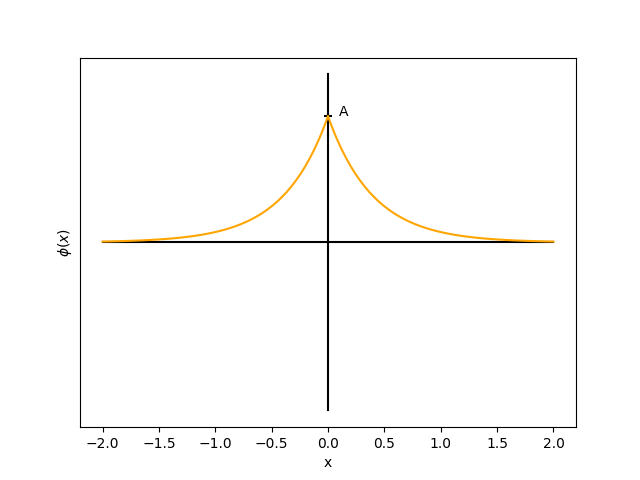
\includegraphics{images4/phi(x).png}
  \centering
  \caption{Solution for g=2.5 of phi(x) for the delta function potential.}
  \labfig{figure4-2}
\end{figure}


To solve for A we need to use the property from \ref{3.3}.

\begin{equation}
\label{4.14}
P(x) = \left\{ \begin{array}{lc}
     A^2e^{2gx}    &  x<0  \\
     A^2e^{-2gx}   &  x>0
\end{array}\right.
\end{equation}

\begin{equation}
\label{4.15}
\begin{array}{c}
     \int_{-\infty}^{\infty}P(x) dx = 1
     \\

     \\
     \frac{A^2}{g}=1
     \\

     \\
     A^2 = g
\end{array}
\end{equation}

We have finally solved the problem and the solution is:

\begin{equation}
\label{4.16}
\phi(x) = \left\{ \begin{array}{lcc}
     \sqrt{g}e^{gx}    &  x<0  \\
     \sqrt{g}e^{-gx}   &  x>0
\end{array}\right.
\end{equation}

We will not do examples using this model because is not that usefull, but it will help us understand the next problem better.



\setchapterpreamble[u]{\margintoc}
\chapter{Multiple potentials}

Until this moment we have only work with 1 potential well but if our goal is to understand solids and their properties we need to figure out how our quantum world works with multiple potential.


\section{Definition}

\begin{figure}[H]
  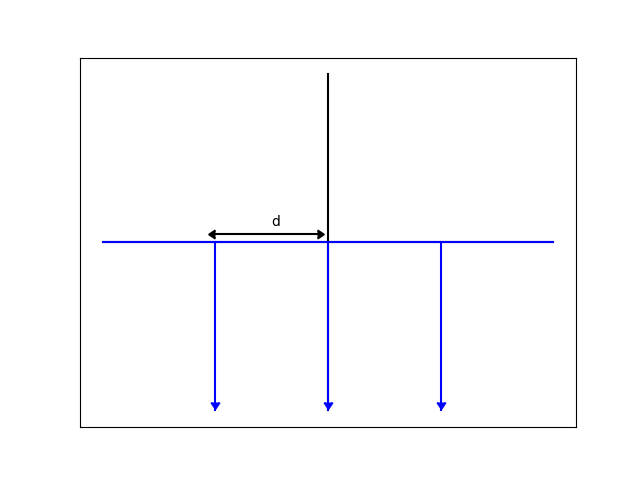
\includegraphics{images5/def.png}
  \centering
  \caption{Multiple delta function potentials problem.}
  \labfig{fig_5.1}
\end{figure}

In this problem we will have N delta function potentials, as the one in the previous chapter, separated by a distance d, with a fix value for g of g=1. The potential can be defined as:

\begin{equation}
  \label{5.1}
  "V(x) = -2 V_0 a \left[\sum_{n=1}^{N} \delta(x-nd) \right]"
\end{equation}

Using \ref{5.1} we get the wave equation for this problem.

\begin{equation}
  \label{5.2}
  "\alpha^2\phi(x) = \frac{\partial^2\phi(x)}{\partial x^2} + 2 g \left[\sum_{n=1}^{N} \delta(x-nd) \right] \phi(x)"
\end{equation}

Outside of the potentials the equation to solve will be the same as \ref{4.6}, our goal is going to be trying to find the relation between the A and B coefficients at both sides of a potential as we can see in \reffig{fig_5.2}

\begin{figure}[H]
  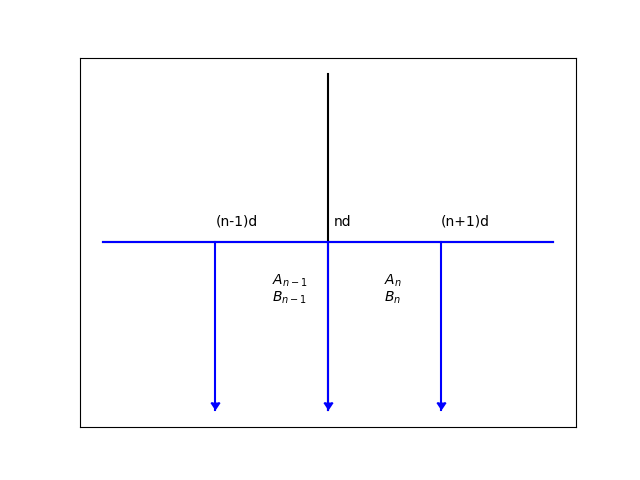
\includegraphics{images5/def_n.png}
  \centering
  \caption{Coefficients outside of the potentials near x=nd.}
  \labfig{fig_5.2}
\end{figure}

\section{Solution}

First, if we look at the limits when n=0 and n=N we get the solutions from the previous chapter.

\begin{equation}
  \label{5.3}
  \begin{array}{l}
    A_0 = 0 \\
    B_N = 0
  \end{array}
\end{equation}

We will use the continuity of $\phi(x)$ to relate the A and B coefficients.

The first condition is that $\phi(x)$ is continuous. To simplify we will use $v = e^{-\alpha\frac{d}{2}}$.



% \setchapterimage[6cm]{seaside}
% \setchapterpreamble[u]{\margintoc}
% \chapter{Page Design}
% \labch{layout}

% \section{Headings}

% So far, in this document I used two different styles for the chapter
% headings: one has the chapter name, a rule and, in the margin, the
% chapter number; the other has an image at the top of the page, and the
% chapter title is printed in a box (like for this chapter). There is one
% additional style, which I used only in the \nrefch{appendix}; there, the chapter title is enclosed in two
% horizontal rules, and the chapter number (or letter, in the case of the
% appendix) is above it.\sidenote{To be honest, I do not think that mixing
% heading styles like this is a wise choice, but in this document I did it
% only to show you how they look.}

% Every book is unique, so it makes sense to have different styles from
% which to choose. Actually, it would be awesome if whenever a
% \Class{kao}-user designs a new heading style, he or she added it to the
% three styles already present, so that it will be available for new users
% and new books.

% The choice of the style is made simple by the \Command{setchapterstyle}
% command. It accepts one option, the name of the style, which can be:
% \enquote{plain}, \enquote{kao}, \enquote{bar}, or
% \enquote{lines}.\sidenote{Plain is the default \LaTeX\xspace title
% style; the other ones are self explanatory.} If instead you want the
% image style, you have to use the command \Command{setchapterimage},
% which accepts the path to the image as argument; you can also provide an
% optional parameter in square brackets to specify the height of the
% image. \Command{setchapterimage} automatically sets the chapter style to
% \enquote{bar} for that chapter (and also for subsequent chapters).

% Let us make some examples. In this book, I begin a normal chapter with
% the lines:
% \begin{lstlisting}
% \setchapterstyle{kao}
% \setchapterpreamble[u]{\margintoc}
% \chapter{Title of the Chapter}
% \labch{title}
% \end{lstlisting}

% In Line 1 I choose the style for the title to be \enquote{kao}. Then, I
% specify that I want the margin toc. The rest is ordinary administration
% in \LaTeX, except that I use my own \Command{labch} to label the
% chapter. Actually, the \Command{setchapterpreamble} is a standard
% \KOMAScript\xspace one, so I invite you to read about it in the KOMA
% documentation. Once the chapter style is set, it holds until you change
% it.\sidenote{The \Command{margintoc} has to be specified at every
% chapter. Perhaps in the future this may change; it all depends on how
% this feature will be welcomed by the users, so keep in touch with me if
% you have preferences!} Whenever I want to start a chapter with an image,
% I simply write:

% \begin{lstlisting}
% \setchapterimage[7cm]{path/to/image.png} % Optionally specify the height
% \setchapterpreamble[u]{\margintoc}
% \chapter{Catchy Title} % No need to set a chapter style
% \labch{catchy}
% \end{lstlisting}

% If you prefer, you can also specify the style at the beginning of the
% main document, and that style will hold until you change it again.

% \section{Headers \& Footers}

% Headers and footers in \KOMAScript\xspace are handled by the
% \Package{scrlayer-scrpage} package. There are two basic style:
% \enquote{scrheadings} and \enquote{plain.scrheadings}. The former is
% used for normal pages, whereas the latter is used in title pages (those
% where a new chapter starts, for instance) and, at least in this book, in
% the front matter. At any rate, the style can be changed with the
% \Command{pagestyle} command, \eg
% \lstinline|\pagestyle{plain.scrheadings}|.

% In both styles, the footer is completely empty. In plain.scrheadings,
% also the header is absent (otherwise it wouldn't be so plain\ldots), but
% in the normal style the design is reminiscent of the \enquote{kao} style
% for chapter titles.

% \begin{kaobox}[frametitle=To Do]
% The \Option{twoside} class option is still unstable and may lead to
% unexpected behaviours. As always, any help will be greatly appreciated.
% \end{kaobox}

% \section{Table of Contents}

% Another important part of a book is the table of contents. By default,
% in \Class{kaobook} there is an entry for everything: list of figures,
% list of tables, bibliographies, and even the table of contents itself.
% Not everybody might like this, so we will provide a description of the
% changes you need to do in order to enable or disable each of these
% entries. In the following \reftab{tocentries}, each item corresponds to
% a possible entry in the \acrshort{tocLabel}, and its description is the
% command you need to provide to have such entry. These commands are
% specified in the attached \href{style/style.sty}{style
% package},\sidenote{In the same file, you can also choose the titles of
% these entries.} so if you don't want the entries, just comment the
% corresponding lines.

% Of course, some packages, like those for glossaries and indices, will
% try to add their own entries.\marginnote{In a later section, we will see
% how you can define your own floating environment, and endow it with an
% entry in the \acrshort{tocLabel}.} In such cases, you have to follow the
% instructions specific to that package. Here, since we have talked about
% glossaries and notations in \refch{references}, we will briefly see how
% to configure them.

% \begin{table}
% \footnotesize
% \caption{Commands to add a particular entry to the table of contents.}
% \labtab{tocentries}
% \begin{tabular}{ l l }
% 	\toprule
% 	Entry & Command to Activate \\
% 	\midrule
% 	Table of Contents & \lstinline|\setuptoc{toc}{totoc}| \\
% 	List of Figs and Tabs & \lstinline|\PassOptionsToClass{toc=listof}{\@baseclass}| \\
% 	Bibliography & \lstinline|\PassOptionsToClass{toc=bibliography}{\@baseclass}| \\
% 	\bottomrule
% \end{tabular}
% \end{table}

% For the \Package{glossaries} package, use the \enquote{toc} option when
% you load it: \lstinline|\usepackage[toc]{glossaries}|. For
% \Package{nomencl}, pass the \enquote{intoc} option at the moment of
% loading the package. Both \Package{glossaries} and \Package{nomencl} are
% loaded in the attached \href{style/packages.sty}{\enquote{packages}
% package}.

% Additional configuration of the table of contents can be performed
% through the packages \Package{etoc}, which is loaded because it is
% needed for the margintocs, or the more traditional \Package{tocbase}.
% Read the respective documentations if you want to be able to change the
% default \acrshort{tocLabel} style.\sidenote[][*-1]{(And please, send me
% a copy of what you have done, I'm so curious!)}

% \section{Paper Size}

% Recent versions of Kaobook support paper sizes different from the
% default A4. It is possible to pass the name of the paper as an option
% to the class, as we are accustomed for any other \LaTeX\ class. For
% example, the class option \Option{b5paper} would set the paper size
% to the B5 format.

% We also support the paper sizes specified in
% \href{https://www.bod.de/hilfe/hilfe-und-service.html?cmd=SINGLE\&entryID=2494\_GER\_WSS\&eo=2\&title=welche-buchformate-gibt-es}{this
% web page} and some additional sizes requested by the users, with the
% option names specified in \reftab{papersizes}.

% \begin{margintable}[*-6]
% 	\caption{Some non-standard paper sizes supported by kaobook.}
% 	\labtab{papersizes}
% 	\begin{tabular}{ll}
% 		\toprule
% 		Dimension & Option name \\
% 		\midrule
% 		12.0cm x 19.0cm & smallpocketpaper \\
% 		13.5cm x 21.5cm & pocketpaper \\
% 		14.8cm x 21.0cm & a5paper \\
% 		15.5cm x 22.0cm & juvenilepaper \\
% 		17.0cm x 17.0cm & smallphotopaper \\
% 		21.0cm x 15.0cm & appendixpaper \\
% 		17.0cm x 22.0cm & cookpaper \\
% 		19.0cm x 27.0cm & illustratedpaper \\
% 		17.0cm x 17.0cm & photopaper \\
% 		16.0cm x 24.0cm & f24paper \\
% 		%21.0cm x 29.7cm & a4paper \\
% 		\bottomrule
% 	\end{tabular}
% \end{margintable}

% For instance, to use the \enquote{smallpocketpaper} add the correct
% description at the beginning of the documentclass instruction:
% \begin{lstlisting}
% \documentclass[
% 		smallpocketpaper,
% 		fontsize=10pt,
% 		twoside=false,
% 		%open=any,
% 		secnumdepth=1,
% ]{kaobook}
% \end{lstlisting}

% \section{Page Layout}

% Besides the page style, you can also change the width of the content of
% a page. This is particularly useful for pages dedicated to part titles,
% where having the 1.5-column layout might be a little awkward, or for
% pages where you only put figures, where it is important to exploit all
% the available space.

% In practice, there are two layouts: \enquote{wide} and \enquote{margin}.
% The former suppresses the margins and allocates the full page for
% contents, while the latter is the layout used in most of the pages of
% this book, including this one. The wide layout is also used
% automatically in the front and back matters.

% \marginnote{Sometimes it is desirable to increase the width for just one
% or a few paragraphs; the \Environment{widepar} environment does that:
% wrap your paragraphs in this environment, and they will occupy the full
% width of the page.}

% To change page layout, use the \Command{pagelayout} command. For
% example, when I start a new part, I write:

% \begin{lstlisting}
% \pagelayout{wide}
% \addpart{Title of the New Part}
% \pagelayout{margin}
% \end{lstlisting}

% Beyond these two basic layouts, it is also possible to finely tune the
% page layout by redefining the \Command{marginlayout} command. This
% command is called internally by the higher-level \Command{pagelayout},
% and it is responsible for setting the width of the margins and of the
% text. The default definition is:

% \begin{lstlisting}
% \newcommand{\marginlayout}{%
% 	\newgeometry{
% 		top=27.4mm,				% height of the top margin
% 		bottom=27.4mm,			% height of the bottom margin
% 		inner=24.8mm,			% width of the inner margin
% 		textwidth=107mm,		% width of the text
% 		marginparsep=8.2mm,		% width between text and margin
% 		marginparwidth=49.4mm,	% width of the margin
% 	}%
% }
% \end{lstlisting}

% so if you want to, say, decrease the width of the margin while
% increasing the width of the text, you could write in the preamble of
% your document something like:

% \begin{lstlisting}
% \renewcommand{\marginlayout}{%
% 	\newgeometry{
% 		top=27.4mm,				% height of the top margin
% 		bottom=27.4mm,			% height of the bottom margin
% 		inner=24.8mm,			% width of the inner margin
% 		textwidth=117mm,		% width of the text
% 		marginparsep=8.2mm,		% width between text and margin
% 		marginparwidth=39.4mm,	% width of the margin
% 	}%
% }
% \end{lstlisting}

% where the text width has been increased by 10mm and the margin width has
% been decreased by 10mm.

% \section{Numbers \& Counters}

% In this short section we shall see how dispositions, sidenotes and
% figures are numbered in the \Class{kaobook} class.

% By default, dispositions are numbered up to the section in \Class{kaobook}
% and up to the subsection in \Class{kaohandt}. This can be changed by
% passing the option \Option{secnumdepth} to\Class{kaobook} or
% \Class{kaohandt} (e.g. 1 corresponds to section and 2 corresponds to
% subsections).

% The sidenotes counter is the same across all the document, but if you
% want it to reset at each chapter, just uncomment the line

% \begin{lstlisting}[style=kaolstplain]
% \counterwithin*{sidenote}{chapter}
% \end{lstlisting}

% in the \Package{styles/style.sty} package provided by this class.

% Figure and Table numbering is also per-chapter; to change that, use
% something like:

% \begin{lstlisting}[style=kaolstplain]
% \renewcommand{\thefigure}{\arabic{section}.\arabic{figure}}
% \end{lstlisting}

% \section{White Space}

% One of the things that I find most hard in \LaTeX\xspace is to finely
% tune the white space around objects. There are not fixed rules, each
% object needs its own adjustment. Here we shall see how some spaces are
% defined at the moment in this class.\marginnote{Attention! This section
% may be incomplete.}

% \textbf{Space around sidenotes and citations marks}

% There should be no space before or after sidenotes and citation marks,
% like so:

% sidenote\sidenote{This paragraph can be used to diagnose any problems:
% if you see whitespace around sidenotes or citation marks, probably
% a \% sign is missing somewhere in the definitions of the class
% macros.}sidenote\newline
% citation\cite{James2013}citation

% \textbf{Space around figures and tables}

% \begin{lstlisting}[style=kaolstplain]
% \renewcommand\FBaskip{.4\topskip}
% \renewcommand\FBbskip{\FBaskip}
% \end{lstlisting}

% \textbf{Space around captions}

% \begin{lstlisting}[style=kaolstplain]
% \captionsetup{
% 	aboveskip=6pt,
% 	belowskip=6pt
% }
% \end{lstlisting}

% \textbf{Space around displays (\eg equations)}

% \begin{lstlisting}[style=kaolstplain]
% \setlength\abovedisplayskip{6pt plus 2pt minus 4pt}
% \setlength\belowdisplayskip{6pt plus 2pt minus 4pt}
% \abovedisplayskip 10\p@ \@plus2\p@ \@minus5\p@
% \abovedisplayshortskip \z@ \@plus3\p@
% \belowdisplayskip \abovedisplayskip
% \belowdisplayshortskip 6\p@ \@plus3\p@ \@minus3\p@
% \end{lstlisting}


\setchapterpreamble[u]{\margintoc}
\chapter{Algebra: Linear vector space}

This chapter will explain and define some mathematic concepts we will used to solve problems with more complicated.

\section{Definition of linear vector space}

A linear vector space is a space where each element of the space is a entry in the space. We will follow the notation for quantum mechanics, where:

\begin{itemize}
  \item $\ket{v}$         Dirac notation for a vector
  \item $\bra{v}$         Conjugate of the vector
  \item $\braket{v}{v}$   Inner product
\end{itemize}

We can use n-special vector to write down all vector of a space n-dimensional.

\begin{equation}
  \label{6.1}
  \bracket{e_i}{e_j} = \delta_{i,j}
\end{equation}

This vectors are called unit vectores, with them we can write any vector as:

\begin{equation}
  \label{6.2}
  \ket{v} = \sum_{i=1}^{n} v_i \ket{e_i}
\end{equation}

We can get any elemnt of v usign this definitions.

\begin{equation}
  \label{6.3}
  \braket{e_j}{v} = \sum_{i=1}^{n} v_i \braket{e_j}{e_i} = v_j
\end{equation}

All this operations can be done because every linear vector must follow:

\begin{equation}
  \label{6.4}
  \braket{v}{(a\ket{w}+b\ket{w})} = a \braket{v}{w} + b\braket{v}{w}
\end{equation}

As we have a definition for $\ket{v}$, we wat one for $\bra{v}$.

\begin{equation}
  \label{6.5}
  \bra{v} = \sum_{i=1}^{n} v_i^{*}\bra{e_i}
\end{equation}

We can know prove that the inner product is greater or equal to 0.

\begin{equation}
  \label{6.6}
  \braket{v}{v} = (\sum_{i=1}^{n} v_i^{*}\bra{e_i})(\sum_{j=1}^{n} v_j \ket{e_j}) = \sum_{i,j=1}^{n} v_i^{*} v_j \braket{e_i}{e_j} = \sum_{i,j=1}^{n} v_i^{*} v_i \geq 0
\end{equation}

And also we have proved that the inner product can only be 0 if $\ket{v} = 0$, and it is called null vector.

Other property of the inner product:


\begin{equation}
  \label{6.7}
  \braket{w}{v} = (\braket{v}{w})^{*}
\end{equation}

We can define a unit vector in direction v as:

\begin{equation}
  \label{6.8}
\ket{\hat{v}} = \frac{1}{\sqrt{\braket{v}{v}}} \ket{v}
\end{equation}

\section{Inequations}

In two dimensional space the inner product is given by the angle between the two vectors.

\begin{equation}
  \label{6.9}
  \begin{array}{c}
    \vec{v_1} \cdot \vec{v_2} = \sqrt{\vec{v_1}\cdot\vec{v_1}} \sqrt{\vec{v_2}\cdot\vec{v_2}} \cos(\theta)
    \\
    (\vec{v_1} \cdot \vec{v_2})(\vec{v_2} \cdot \vec{v_1}) = (\vec{v_1}\cdot\vec{v_1})  (\vec{v_2}\cdot\vec{v_2}) \cos^2(\theta) \leq (\vec{v_1}\cdot\vec{v_1})  (\vec{v_2}\cdot\vec{v_2})
  \end{array}
\end{equation}

This is known as Schwarz Inequation and can be generalize to every number of dimensions.

\begin{equation}
  \label{6.10}
  \begin{array}{c}
    \braket{w}{v}\braket{v}{w} \leq \braket{v}{v} \braket{w}{w}
  \end{array}
\end{equation}

Now we want a relation between the sum of an inner product and it's conjugate.

\begin{equation}
  \label{6.11}
  \braket{w}{v}+\braket{v}{w} \leq 2 \sqrt{\braket{v}{v} \braket{w}{w}}
\end{equation}

Using \ref{6.11} and \ref{6.10} we can get the Triangle Inequality.

\begin{equation}
  \label{6.12}
  \begin{array}{c}
    (\bra{w}+\bra{v})(\ket{w}+\ket{v}) = \braket{w}{w}+\braket{v}{v}+\braket{v}{w}+\braket{w}{v}
    \\

    \\
    (\bra{w}+\bra{v})(\ket{w}+\ket{v}) \leq \sqrt{\braket{w}{w}}^2 + \sqrt{\braket{v}{v}}^2 + 2 \sqrt{\braket{w}{w}} \sqrt{\braket{v}{v}}
    \\

    \\
    \sqrt{(\bra{w}+\bra{v})(\ket{w}+\ket{v})} \leq \sqrt{\braket{w}{w}} + \sqrt{\braket{v}{v}}
    \\

    \\
    Norm(\ket{w}+\ket{v}) \leq Norm(\ket{w}) + Norm(\ket{v})
  \end{array}
\end{equation}

\section{Definitions in Wave Mechanicsand Operators}

In our physical aproach $\ket{e_i}$ is a normalize function in one or more dimension, $\bra{e_i}$ is the conjugate of the function and $\braket{e_i}{e_j}$ is the inner product, define as an integral over all space.

We can rewrite the wave equations for each energy, E_i.

\begin{equation}
\label{6.13}
\left[-\frac{\hbar^2}{2m} \frac{d^2}{dx^2}+ V(x) \right] \phi_i(x) = [E_i] \phi_i(x)
\end{equation}

Where the left part in brackets is a linear operator in our vector space and is acting an element giving as a result a proportionality with him self.

We have introduced a new concept, the linear operatorr. We say an operator is linear if:

\begin{equation}
  \label{6.14}
  \begin{array}{c}
    A \ket{v} = \ket{w} \\
    A(\alpha_1 \ket{v_1}+\alpha_2\ket{v_2}) = \alpha_1 A \ket{v_1} + \alpha_2 A \ket{v_2}
  \end{array}
\end{equation}

Where $\alpha_1$, $\alpha_2$ are complex numbers. As we did with vectors we have to established some rules.

\begin{equation}
  \label{6.15}
  A \ket{e_i} = \sum_{j} \ket{e_j} A_{ji}
\end{equation}

Given A and the vectors that define our space, $\ket{e_i}$, we can find $A_{ij}$.

\begin{equation}
  \label{6.16}
  \bra{e_k}(A \ket{e_i}) =\bra{e_k}(\sum_{j}\ket{e_j}A_{ji}) = \sum_{j} (\braket{e_k}{e_j})Aji = \sum_{j}\delta_{kj}A_{ji}=A_{ki}
\end{equation}

One consequence of this result is the matrix multiplication acting on components.

\begin{equation}
  \label{6.17}
  \begin{array}{c}
    \ket{w} = A \ket{v} = A \sum_{i} v_i\ket{e_i} = \sum_{i} v_i\sum_{j}\ket{e_j}A_{ji} = \sum_j\sum_i A_{ji} v_i \ket{e_j} = \sum_{j} w_i \ket{e_j}\\
    w_j = \sum_{i}A_{ji} v_i
  \end{array}
\end{equation}

We can aply more than one operator to a vector.

\begin{equation}
  \label{6.18}
  \begin{array}{c}
    \ket{w} = A(B \ket{v}) \\
    w_j = \sum_{i}(A_{ji}(B\ket{v})_i) = \sum_{k}\sum{i}A_{ji}B_{ik}v_k = \sum_{k} (AB)_{jk} v_k
  \end{array}
\end{equation}

In general A and B do not commute.

\begin{equation}
  \ket{x} = (AB-BA) \ket{v}
\end{equation}

We call that difference of the multiplication of the operators, a commutator. It has the property:

\begin{equation}
  \begin{array}{c}
    [A,\alpha B + \beta C]\ket{v} = (A(\alpha B+\beta C)-(\alpha B + \beta C)A)\ket{v} =
    \\
    = (\alpha AB+\beta AC-\alpha BA - \beta CA) \ket{v} =
    \\
    = (\alpha (AB-BA)+\beta(AC-CA)) \ket{v}
  \end{array}
\end{equation}

This mean that:

\begin{equation}
    [A,\alpha B + \beta C] = \alpha [A,B] + \beta[A,C]
\end{equation}

There is also a rule with the product of two operators.

\begin{equation}
  \begin{array}{c}
    [A,BC] = ABC - BCA - BAC + BAC =
    \\
    = (AB-BA)C + B(AC-CA) =
    \\
    = [A,B]C + B[A,C]
  \end{array}
\end{equation}

We called operator adjunt to A to $A^{\dagger}$ if:

\begin{equation}
  \begin{array}{c}
    A \ket{v} = \ket{w}
    \\
    \bra A^{\dagger} = \bra{w}
  \end{array}
\end{equation}

$A^{\dagger}$ is the transpose complex conjugate of the operator A.

\begin{equation}
  A^{\dagger} = (A^{\star})^{T} = (A^{T})^{\star}
\end{equation}

If $A=A^{\dagger}$ A is called hermitian

If $A=-A^{\dagger}$ A is called anti-hermitian

We define the identity operator, I, as:

\begin{equation}
  (I)_{ij} = \left\{
  \begin{array}{lc}
    1 & i=j
    \\
    0 & i \neq j
  \end{array}
  \right.
\end{equation}

If $A A^{\dagger} = I$ we say that A is a unitary operator.

We can also prove that $(AB)^{\dagger} = (B^{\dagger}A^{\dagger})$.

\begin{equation}
  \begin{array}{c}
    (AB)^{\dagger} = ((AB)^T)^* = (B^TA^T)^*= (B^T)^*(A^T)^* = B^\dagger A^\dagger
  \end{array}
\end{equation}

Considering a hermitian operator H that satisfy:

\begin{equation}
  H\ket{h_i} = h_i \ket{h_i}
\end{equation}

Where $\ket{h_i}$ is an eigenvector such that the action of the operator on it, returns a vector proportional to itself with $h_i$ as the proportionality (eigenvalue).

We can prove that the eigenvalue is a real number.

\begin{equation}
  \begin{array}{c}
    \bra{h_i}H^{\dagger} = h_i^* \bra{h_i}
    \\
    \bra{h_i}H^{\dagger} = h_i^* \bra{h_i}
    \\
    \bra{h_i}H\ket{h_i} = h_i \braket{h_i}{h_i}
    \\
    \bra{h_i}H\ket{h_i} = h_i^* \braket{h_i}{h_i}
  \end{array}
\end{equation}

We can also prove that the different eigenvectors are orthogonal.

\begin{equation}
  \begin{array}{c}
    \bra{h_j}H\ket{h_i} = h_j \braket{h_i}{h_j}
    \\
    \bra{h_j}H\ket{h_i} = h_i \braket{h_i}{h_j}
    \\
    (h_i-h_j)\braket{h_j}{h_i} = 0
  \end{array}
\end{equation}

If $h_i\neq h_j$ then the eigenvectors are orthogonal. In one dimensional problems we don't have problems because the eigenvalues are unique, we will talk about what happen when they are equal later when we introduce more dimensions.

It can be prove that the set of eigenvectors form a base.

\begin{equation}
  \begin{array}{c}
    PROVE \braket{h_i}{h_i} = 1 NOT PROVE YET
  \end{array}
\end{equation}

Coming back to physics with all this properties we will define our inner product and our operator.

\begin{equation}
  \bra{\psi(x)}A\ket{\phi(x)} = \int_{-\infty}^{\infty}\psi^*(x)\left[\frac{d^2}{dx^2}\phi(x)\right]dx
\end{equation}

Where our inner product is the integral of the product of the functions and the operator is the second derivative. We can prove that in this inner product our operator is hermitian with the limits $\phi(\pm \infty) = 0$ and $\psi(\pm \infty) = 0$.

\begin{equation}
  \begin{array}{c}
    \int_{-\infty}^{\infty}\psi^*(x)\left[\frac{d^2}{dx^2}\phi(x)\right] dx = \int_{-\infty}^{\infty} \frac{d}{dx}\left[\psi^*\frac{d}{dx}\phi\right]-\frac{d\psi^*}{dx}\frac{d\phi}{dx} dx =
    \\

    \\
    \left.\psi^*\frac{d\phi}{dx}\right|_{-\infty}^{\infty} - \int_{-\infty}^{\infty} \frac{d\psi^*}{dx}\frac{d\phi}{dx} dx = -\int_{-\infty}^{\infty} \frac{d}{dx}\left(\frac{d\psi^*}{dx}\phi\right)-\frac{d^2\psi^*}{dx^2}\phi dx =
    \\

    \\
    =\left.\frac{d\psi^*}{dx}\phi\right|_{-\infty}^{\infty} + \int_{-\infty}^{\infty} \left[\frac{d^2\psi^*}{dx^2}\right]^2\phi dx
  \end{array}
\end{equation}

We have proved that:

\begin{equation}
  \bra{\psi(x)}\left(\frac{d^2}{dx^2}\ket{\phi}\right) = \left(\bra{\psi(x)}\frac{d^2}{dx^2}\right)\ket{\phi}
\end{equation}

This means that the operator is hermitian. And it will be also hermitian if we multiply by a real number and add a real number thats why we can say that our operator for the Schrödinger wave equation is hermitian if V(x) is real.

\begin{equation}
  \left[\frac{-\hbar^2}{2m}\frac{d^2}{dx^2}+V(x)\right]\ket{E_i} = E_i \ket{E_i}
\end{equation}

We will need also to explore how the operator d/dx behaves.

\begin{equation}
  \begin{array}{c}
    \int_{-\infty}^{\infty}\psi^*(x)\left[\frac{d}{dx}\phi(x)\right] dx = \int_{-\infty}^{\infty} \frac{d}{dx}\left[\psi^* \phi\right]-\left(\frac{d\psi^*}{dx}\right) \phi dx =
    \\

    \\
    \left.\psi^*\phi\right|_{-\infty}^{\infty} + \int_{-\infty}^{\infty} \left(-\frac{d}{dx}\psi^*\right)\phi dx = \int_{-\infty}^{\infty} \left(-\frac{d}{dx}\psi^*\right)\phi dx
    \\

    \\
    \left(\frac{d}{dx}\right)^{\dagger} = -\frac{d}{dx}
  \end{array}
\end{equation}

We have proved that this operator is anti-hermitian.

% \setchapterstyle{kao}
% %\setchapterpreamble[u]{\margintoc}
% \chapter{References}
% \labch{references}

% \section{Citations}

% \index{citations}
% To cite someone \sidecite{Visscher2008,James2013} is very simple: just
% use the \Command{sidecite}\index{\Command{sidecite}} command. It does
% not have an offset argument yet, but it probably will in the future.
% This command supports multiple entries, as you can see, and by default
% it prints the reference on the margin as well as adding it to the
% bibliography at the end of the document. Note that the citations have
% nothing to do with the text,\sidecite{James2013} but they are completely
% random as they only serve the purpose to illustrate the feature.

% For this setup I wrote a separate package, \Package{kaobiblio}, which
% you can find in the \Package{styles} directory and include in your main
% tex file. This package accepts all the options that you can pass to
% \Package{biblatex}, and actually it passes them to \Package{biblatex}
% under the hood. Moreover, it also defines some commands, like
% \Command{sidecite}, and environments that can be used within a
% \Class{kao} book.\sidenote[][-.9cm]{For this reason you should always
% use \Package{kaobiblio} instead of \Package{biblatex}, but the syntax
% and the options are exactly the same.}

% If you want to use \Package{bibtex} instead of \Package{biblatex},
% pass the option \Option{backend=bibtex} to \Package{kaobiblio}.
% \Package{kaobiblio} also supports two options that are not shared with
% \Package{biblatex}: \Option{addspace} and \Option{linkeverything},
% both of which are boolean options, meaning that they can take
% either \enquote{true} or \enquote{false} as a value. If you
% pass \Option{addspace=true} when loading \Package{kaobiblio},
% a space will be automatically added before the citation marks.
% If you pass \Option{linkeverything=true}, the author's name in
% the authoryear-* and authortitle-* styles will be a hyperlink
% like the year.\sidenote{The fact that the author name is not
% a hyperlink bothers more than one biblatex user. There are
% \href{https://github.com/plk/biblatex/issues/428}{strong arguments}
% \emph{against} hyperlinking the author name, but in my personal opinion,
% linking the author's name does not result in any problems in most
% practical cases.}

% As you have seen, the \Command{sidecite} command will print a citation
% in the margin. However, this command would be useless without a way to
% customise the format of the citation, so the \Class{kaobook} provides
% also the \Command{formatmargincitation} command. By \enquote{renewing}
% that command, you can choose which items will be printed in the margins.
% The best way to understand how it works is to see the actual definition
% of this command.

% \begin{lstlisting}[style=kaolstplain,linewidth=1.5\textwidth]
% \newcommand{\formatmargincitation}[1]{%
% 	\parencite{#1}: \citeauthor*{#1} (\citeyear{#1}), \citetitle{#1}%
% }
% \end{lstlisting}

% Thus, the \Command{formatmargincitation} accepts one parameter, which is
% the citation key, and prints the parencite followed by a colon, then the
% author, then the year (in brackets), and finally the
% title.\sidecite{Battle2014} Now, suppose that you wish the margin
% citation to display the year and the author, followed by the title, and
% finally a fixed arbitrary string; you would add to your document:

% \begin{lstlisting}[style=kaolstplain,linewidth=1.5\textwidth]
% \renewcommand{\formatmargincitation}[1]{%
% 	\citeyear{#1}, \citeauthor*{#1}: \citetitle{#1}; very interesting!%
% }
% \end{lstlisting}

% \renewcommand{\formatmargincitation}[1]{%
% 	\citeyear{#1}, \citeauthor*{#1}: \citetitle{#1}; very interesting!%
% }

% The above code results in citations that look like the
% following.\sidecite{Zou2005} Of course, changing the format is most
% useful when you also change the default bibliography style. For
% instance, if you want to use the \enquote{philosophy-modern} style for
% your bibliography, you might have something like this in the preamble:

% \begin{lstlisting}[style=kaolstplain,linewidth=1.5\textwidth]
% \usepackage[style=philosophy-modern]{styles/kaobiblio}
% \renewcommand{\formatmargincitation}[1]{%
% 	\sdcite{#1}%
% }
% \addbibresource{main.bib}
% \end{lstlisting}

% \renewcommand{\formatmargincitation}[1]{%
% 	\parencite{#1}: \citeauthor*{#1} (\citeyear{#1}), \citetitle{#1}%
% }

% The commands like \Command{citeyear}, \Command{parencite}
% and \Command{sdcite} are just examples. A full
% reference of the available commands can be found in this
% \href{http://tug.ctan.org/info/biblatex-cheatsheet/biblatex-cheatsheet.pdf}{cheatsheet},
% under the \enquote{Citations} section.

% Finally, to compile a document containing citations, you need to use an
% external tool, which for this class is biber. You need to run the
% following (assuming that your tex file is called main.tex):

% \begin{lstlisting}[style=kaolstplain]
% $ pdflatex main
% $ biber main
% $ pdflatex main
% \end{lstlisting}

% \section{Glossaries and Indices}

% \index{glossary}
% The \Class{kaobook} class loads the packages \Package{glossaries} and
% \Package{imakeidx}, with which you can add glossaries and indices to
% your book. For instance, I previously defined some glossary entries and
% now I am going to use them, like this: \gls{computer}.
% \Package{glossaries} also allows you to use acronyms, like the
% following: this is the full version, \acrfull{fpsLabel}, and this is the
% short one \acrshort{fpsLabel}. These entries will appear in the glossary
% in the backmatter.

% Unless you use \href{https://www.overleaf.com}{Overleaf} or some other
% fancy IDE for \LaTeX, you need to run an external command from your
% terminal in order to compile a document with a glossary. In particular,
% the commands required are:\sidenote{These are the commands you would run
% in a UNIX system, but see also \nrefsec{compiling}; I have no idea about
% how it works in Windows.}

% \begin{lstlisting}[style=kaolstplain]
% $ pdflatex main
% $ makeglossaries main
% $ pdflatex main
% \end{lstlisting}

% Note that you need not run \texttt{makeglossaries} every time you
% compile your document, but only when you change the glossary entries.

% \index{index}
% To create an index, you need to insert the command
% \lstinline|\index{subject}| whenever you are talking about
% \enquote{subject} in the text. For instance, at the start of this
% paragraph I would write \lstinline|index{index}|, and an entry would be
% added to the Index in the backmatter. Check it out!

% \marginnote[2mm]{In theory, you would need to run an external command
% for the index as well, but luckily the package we suggested,
% 	\Package{imakeidx}, can compile the index automatically.}

% \index{nomenclature}
% A nomenclature is just a special kind of index; you can find one at the end of
% this book. To insert a nomenclature, we use the package \Package{nomencl} and
% add the terms with the command \Command{nomenclature}. We put then a
% \Command{printnomenclature} where we want it to appear.

% Also with this package we need to run an external command to compile the
% document, otherwise the nomenclature will not appear:

% \begin{lstlisting}[style=kaolstplain]
% $ pdflatex main
% $ makeindex main.nlo -s nomencl.ist -o main.nls
% $ pdflatex main
% \end{lstlisting}

% These packages are all loaded in
% \href{style/packages.sty}{packages.sty}, one of the files that come with
% this class. However, the configuration of the elements is best done in
% the main.tex file, since each book will have different entries and
% styles.

% Note that the \Package{nomencl} package caused problems when the
% document was compiled, so, to make a long story short, I had to prevent
% \Package{scrhack} to load the hack-file for \Package{nomencl}. When
% compiling the document on Overleaf, however, this problem seem to
% vanish.

% \marginnote[-19mm]{This brief section was by no means a complete
% reference on the subject, therefore you should consult the documentation
% of the above package to gain a full understanding of how they work.}

% \section{Hyperreferences}
% \labsec{hyprefs}

% \index{hyperreferences}
% Together with this class we provide a handy package to help you
% referencing the same elements always in the same way, for consistency
% across the book. First, you can label each element with a specific
% command. For instance, should you want to label a chapter, you would put
% \lstinline|\labch{chapter-title}| right after the \Command{chapter}
% directive. This is just a convenience, because \Command{labch} is
% actually just an alias to \lstinline|\label{ch:chapter-title}|, so it
% spares you the writing of \enquote{ch:}. We defined similar commands for
% many typically labeled elements, including:

% \begin{multicols}{2}
% \setlength{\columnseprule}{0pt}
% \begin{itemize}
% 	\item Page: \Command{labpage}
% 	\item Part: \Command{labpart}
% 	\item Chapter: \Command{labch}
% 	\item Section: \Command{labsec}
% 	\item Figure: \Command{labfig}
% 	\item Table: \Command{labtab}
% 	\item Definition: \Command{labdef}
% 	\item Assumption: \Command{labassum}
% 	\item Theorem: \Command{labthm}
% 	\item Proposition: \Command{labprop}
% 	\item Lemma: \Command{lablemma}
% 	\item Remark: \Command{labremark}
% 	\item Example: \Command{labexample}
% 	\item Exercise: \Command{labexercise}
% \end{itemize}
% \end{multicols}

% Of course, we have similar commands for referencing those elements.
% However, since the style of the reference should depend on the context,
% we provide different commands to reference the same thing. For instance,
% in some occasions you may want to reference the chapter by name, but
% other times you want to reference it only by number. In general, there
% are four reference style, which we call plain, vario, name, and full.

% The plain style references only by number. It is accessed, for chapters,
% with \lstinline|\refch{chapter-title}| (for other elements, the syntax
% is analogous). Such a reference results in: \refch{references}.

% The vario and name styles rest upon the \Package{varioref} package.
% Their syntax is \lstinline|\vrefch{chapter-title}| and
% \lstinline|\nrefch{chapter-title}|, and they result in:
% \vrefch{references}, for the vario style, and: \nrefch{references}, for
% the name style. As you can see, the page is referenced in
% \Package{varioref} style.

% The full style references everything. You can use it with
% \lstinline|\frefch{chapter-title}| and it looks like this:
% \frefch{references}.

% Of course, all the other elements have similar commands (\eg for parts
% you would use \lstinline|\vrefpart{part-title}| or something like that).
% However, not all elements implement all the four styles. The commands
% provided should be enough, but if you want to see what is available or
% to add the missing ones, have a look at the
% \href{styles/kaorefs.sty}{attached package}.

% In order to have access to all these features, the \Package{kaorefs}
% should be loaded in the preamble of your document. It should be loaded
% last, or at least after \Package{babel} (or \Package{polyglossia}) and
% \Package{plaintheorems} (or \Package{mdftheorems}). Options can be
% passed to it like to any other package; in particular, it is possible to
% specify the language of the captions. For instance, if you specify
% \enquote{italian} as an option, instead of \enquote{Chapter} it will be
% printed \enquote{Capitolo}, the Italian analog. If you know other
% languages, you are welcome to contribute the translations of these
% captions! Feel free to contact the author of the class for further
% details.

% The \Package{kaorefs} package also include \Package{cleveref}, so it is
% possible to use \Command{cref} in addition to all the previously
% described referencing commands.

% \section{A Final Note on Compilation}
% \labsec{compiling}

% Probably the easiest way to compile a latex document is with the
% \Package{latexmk} script, as it can take care of everything, if properly
% configured, from the bibliography to the glossary. The command to issue,
% in general, is:

% \begin{lstlisting}
% latexmk [latexmk_options] [filename ...]
% \end{lstlisting}

% \Package{latexmk} can be extensively configured (see
% \url{https://mg.readthedocs.io/latexmk.html}). For convenience, I print
% here an example configuration that would cover all the steps described
% above.

% \begin{lstlisting}
% # By default compile only the file called 'main.tex'
% @default_files = ('main.tex');

% # Compile the glossary and acronyms list (package 'glossaries')
% add_cus_dep( 'acn', 'acr', 0, 'makeglossaries' );
% add_cus_dep( 'glo', 'gls', 0, 'makeglossaries' );
% $clean_ext .= " acr acn alg glo gls glg";
% sub makeglossaries {
%    my ($base_name, $path) = fileparse( $_[0] );
%    pushd $path;
%    my $return = system "makeglossaries", $base_name;
%    popd;
%    return $return;
% }

% # Compile the nomenclature (package 'nomencl')
% add_cus_dep( 'nlo', 'nls', 0, 'makenlo2nls' );
% sub makenlo2nls {
%     system( "makeindex -s nomencl.ist -o \"$_[0].nls\" \"$_[0].nlo\"" );
% }
% \end{lstlisting}

% However, if you'd rather not use an external package and want to do
% everything manually, here are some tips.\sidenote{As the author only
% uses Linux and compiles everything from the command line, he doesn't
% know how the compilation works in Windows or Mac. The tips, therefore,
% refer to the usage with Linux from the command line.}

% \minisec{Compiling the examples in the kaobook repository}
% To compile the examples, and in particular the documentation, that are
% in the \Path{examples} directory of the
% \href{https://github.com/fmarotta/kaobook}{kaobook repository} on
% GitHub, do as follows. \lstinline[language=bash]|cd| into the root
% directory of the repository, and run
% \lstinline|pdflatex -output-directory examples/documentation main.tex|.
% With this trick, you can compile the documentation using the class files
% pertaining to the repository (and not, say, those in your texmf tree).
% The \enquote{-output-directory} option works with the other
% \LaTeX-related commands such as biber and makeglossaries.

% A note of warning: sometimes \LaTeX\ needs more than one run to get the
% correct position of each element; this is true in particular for the
% positioning of floating elements like figures, tables, and margin notes.
% Occasionally, \LaTeX\ can need up to four re-runs, so If the alignment
% of margin elements looks odd, or if they bleed into ther main text, try
% runnign pdflatex one more time.


\setchapterpreamble[u]{\margintoc}
\chapter{Harmonic Oscilator}

We want to use the algebra we learnt in the previous chaoter, for that we will try to solve the problem where the potential V(x), is a one dimensional harmonic oscilator potential.

\section{Definition}

The potential for an harmonic oscilator in one dimension is given by the expresion:

\begin{equation}
  \begin{array}{cc}
    V(x) = \frac{1}{2} k x^2 & k > 0
  \end{array}
\end{equation}

This potential comes from a force, $F(x) = -k x$, so the units of k are $kg/s^2$. Because of this we can say that:

\begin{equation}
  \omega=\sqrt{\frac{k}{m}}
\end{equation}

Using Newton 3rd Law we can say:

\begin{equation}
  \frac{d^2x}{dt^2}= -\omega^2 x
\end{equation}

Solving this equation we get:

\begin{equation}
  \begin{array}{c}
    x(t) = A \sin(\omega t) + B \cos(\omega t)
    \\
    v(t) = A\omega \cos(\omega t) - B\omega \sin(\omega t)
  \end{array}
\end{equation}

If we define some initial conditions such as $x(0)=x_0$ and $v(0)=0$, we can solve the coeficients, in this case $B=x_0$ and $A=0$.

\begin{equation}
  \begin{array}{c}
    x(t) = x_0 \cos(\omega t)
    \\
    v(t) =  - x_0 \omega \sin(\omega t)
  \end{array}
\end{equation}

And we can define two energies, a potential energy and a kinetic energy. The total energy is going to be the addition of the other two.

\begin{equation}
  \begin{array}{c}
    P.E(t) = \frac{1}{2} k (x(t))^2 = \frac{1}{2} k x_0^2 cos^2(\omega t)
    \\

    \\
    K.E(t) = \frac{1}{2} m (v(t))^2 = \frac{1}{2} m \omega^2 x_0^2 sin^2(\omega t)
    \\

    \\
    T.E(t) = P.E + K.E = \frac{1}{2} k x_0^2 = constant > 0
  \end{array}
\end{equation}

The total energy turn to be constant among time and positive.

\section{Solving the Wave Equation}

The Schrödinger wave equation gets the shape:

\begin{equation}
  \left[\frac{-\hbar^2}{2m}\frac{d^2}{dx^2}+\frac{1}{2}kx^2\right]\phi(x) = E \phi(x)
\end{equation}

Firstly, we will simplify the equation using natural units. We will make a change of variables $x=by$ and try to get the equation for $\phi(bx)=\chi(y)$.

\begin{equation}
  \begin{array}{c}
    \frac{-\hbar^2}{2mb^2}\frac{d^2\chi(y)}{dy^2}+\frac{1}{2}kby^2\chi(y) = E\chi(y)
    \\
    \frac{\hbar^2}{2mb^2} = \frac{1}{2}k b^2
    \\
    b^2 = \frac{\hbar^2}{m\omega}
  \end{array}
\end{equation}

Now that we have the factor to turn into natural units we can rewrite our wave equation. We will also use the definition of the energy given in the second chapter, $E=\hbar \omega$.

\begin{equation}
  \begin{array}{c}
    -\frac{1}{2}\hbar \omega \frac{d^2\chi(y)}{dy^2} + \frac{1}{2} \hbar \omega y^2 \chi(y) = \alpha(\hbar\omega)\chi(y)
    \\
    -\frac{1}{2}\frac{d^2\chi_n}{dy^2}+\frac{1}{2}y^2\chi_n = \alpha_n \chi_n
  \end{array}
\end{equation}

We want to find $\alpha_n$ and it's associate $\chi_n$ for every $n$. We will define the hermitian operator H from the previous equation.

\begin{equation}
  \begin{array}{c}
    \right[-\frac{1}{2}\frac{d^2}{dy^2}+\frac{1}{2}y^2\left]\chi_n = [\alpha_n] \chi_n
    \\
    H \chi_n = [\alpha_n] \chi_n
  \end{array}
\end{equation}

We define the operator $a$ using what we propose in the end of the previous chapter.

\begin{equation}
  \begin{array}{c}
    a=\frac{1}{\sqrt{2}}\left(\frac{d}{dy}+y\right)
    \\

    \\
    a^\dagger = \frac{1}{\sqrt{2}}\left(\left(\frac{d}{dy}\right)^\dagger+(y)^\dagger\right) = \frac{1}{\sqrt{2}}\left(-\frac{d}{dy}+y\right)
    \\

    \\
    (a^\dagger a)f(y) = \left(-\frac{1}{2}\frac{d^2}{dy^2}+\frac{1}{2}y^2-\frac{1}{2}\right)f(y)
  \end{array}
\end{equation}

We will called $a^\dagger a$ a new operator N, i. e. $N=a^\dagger a$. This operator is hermitian.

\begin{equation}
  \begin{array}{c}
    aa^\dagger - a^\dagger a = \left(-\frac{1}{2}\frac{d^2}{dy^2}+\frac{1}{2}y^2+\frac{1}{2}\right) - \left(-\frac{1}{2}\frac{d^2}{dy^2}+\frac{1}{2}y^2-\frac{1}{2}\right) = 1
  \end{array}
\end{equation}

This resolut is interesting for many reason but one of them is that it prove that $a$ can not be represented as a finite matrix.

Summarizing what we have done so far with this operators:

\begin{equation}
  \begin{array}{c}
    \left[ a,a^\dagger \right] = 1
    \\
    \left[ N,a \right] = -a
    \\
    \left[ N,a^{\dagger} \right] = a^\dagger
  \end{array}
\end{equation}

If we go again to the wave equation we have:

\begin{equation}
  \begin{array}{c}
    [a^\dagger a+\frac{1}{2}=\alpha]\chi
    \\
    N\chi = \left(\alpha-\frac{1}{2}\right)\chi
    \\
    aN\chi = \left(\alpha-\frac{1}{2}\right)a\chi
    \\
    N[a\chi]=\left(\alpha-1-\frac{1}{2}\right)a\chi
  \end{array}
\end{equation}

$a\chi$ is an eigenvector with eigenvalue $(\alpha-1)$

We can prove that $\chi$ have infinite solutions.

\begin{equation}
  \begin{array}{c}
    a^\dagger N \chi = \left(\alpha - \frac{1}{2}\right)a^{\dagger}\chi
    \\
    (Na^\dagger-a^\dagger) \chi = \left(\alpha - \frac{1}{2}\right)a^{\dagger}\chi
    \\
    N(a^\dagger\chi)=\left(\alpha+1-\frac{1}{2}\right)(a^\dagger\chi)
  \end{array}
\end{equation}

If $\chi$ has finite solutions, $a$ has to be a finite matrix, and we prove that is not allowed.

\begin{equation}
  \int_{-\infty}^{\infty} f^*(a^\dagger a f)dx = \int_{-\infty}^{\infty} (af)^*(af) dx \geq 0
\end{equation}

Now we know that $\alpha \geq\frac{1}{2}$, so the solutions have a minimum where $\alpha = \frac{1}{2}$ .

We can search now for our first solution.

\begin{equation}
  \begin{array}{c}
    a\chi_0 = 0 =>
    \\
    => \left(\frac{d}{dy}+\frac{1}{2}\right)\chi_0 = 0
    \\
    \left(aa^\dagger+\frac{1}{2}\right)\chi_0 = \frac{1}{2} \chi_0
  \end{array}
\end{equation}

The first two lines represent the lowest solution and the last one is the next solution. With this we get that:

\begin{equation}
  \alpha = n+\frac{1}{2}
\end{equation}

Now we want to calculate $\chi_0$.

\begin{equation}
  \begin{array}{c}
    a\chi_0 = 0
    \\
    \chi_0 = A e^{-\frac{y^2}{2}}
  \end{array}
\end{equation}

We need to find the value for A to normalize the solution.

\begin{equation}
  \begin{array}{c}
    \int_{-\infty}^{\infty} \chi_0 \chi_0 dx = 1
    \\

    \\
    A^2 \int_{-\infty}^{\infty} e^{-y^2} dx = 1
    \\

    \\
    A=\frac{1}{\pi^{\frac{1}{4}}}
  \end{array}
\end{equation}

Our final expresion for $\chi_0$ is:

\begin{equation}
  \begin{array}{c}
    \chi_0 = \frac{1}{\pi^{\frac{1}{4}}} e^{-\frac{y^2}{2}}
  \end{array}
\end{equation}

From this we can say that:

\begin{equation}
  \begin{array}{c}
    N\chi_n = n \chi_n
  \end{array}
\end{equation}

We want to normalize $\chi_n$ so we will ad a normalization factor C, where $a^\dagger\chi_n=C\chi_{n+1}$

\begin{equation}
  \begin{array}{c}
    C^2 \int_{-\infty}^{\infty} \chi^2_{n+1} dy = \int_{-\infty}^{\infty} (a^\dagger\chi_n)(a^\dagger\chi_n)dy = \int_{-\infty}^{\infty} =
    \\

    \\
    = \int_{-\infty}^{\infty}\chi_n(aa^\dagger\chi_n)dy=\int_{-\infty}^{\infty}\chi_n n\chi_n dy + \int_{-\infty}^{\infty}\chi_n^2dy= n+1
    \\

    \\
    C = \sqrt{n+1}
  \end{array}
\end{equation}

We want to redifine $\chi_n$ as:

\begin{equation}
  \chi_n = \frac{H_n(y)}{\sqrt{2\pi}}e^{\frac{-y^2}{2}}
\end{equation}

We want to find H_{n+1} using the previous two equations.

\begin{equation}
  \begin{array}{c}
    a^\dagger \chi_n = C \chi_{n+1} = \sqrt{1+n} \chi_{n+1}
    \\

    \\
    \frac{1}{\sqrt{2}}\left(-\frac{d}{dx}+y\right)\frac{H_n(y)}{\sqrt{2\pi}}e^{\frac{-y^2}{2}} = \sqrt{n+1} \frac{H_{n+1}}{\sqrt{2\pi}}e^{\frac{-y^2}{2}}
    \\

    \\
    \frac{1}{\sqrt{2(n+1)}}\left[-H'(y)e^{\frac{-y^2}{2}}+y H(y)e^\frac{-y^2}{2}+y H(y)e^\frac{-y^2}{2}\right]= H_{n+1} e^\frac{-y^2}{2}
    \\

    \\
    H_{n+1} = \frac{1}{\sqrt{2(n+1)}}\left[-H_n'(y)+2 y H_n(y)\right]
  \end{array}
\end{equation}

Whre $H_0$ is define as $H_0=1$.

Because $\chi_n$ is normalized we can say that $H_n(y)$ are orthonormal polynomials under a Gaussian width.

\begin{equation}
  \begin{array}{c}
    \frac{1}{2\pi}\int_{-\infty}^{\infty} \chi_n(y) \chi_m(y) dy = \delta_{nm}
    \\

    \\
    \frac{1}{2\pi}\int_{-\infty}^{\infty} H_n(y) H_m(y) e^{\frac{-y^2}{2}}dy = \delta_{nm}
  \end{array}
\end{equation}

We called this functions Hermite polynomials.

\begin{figure}[H]
  \centering
  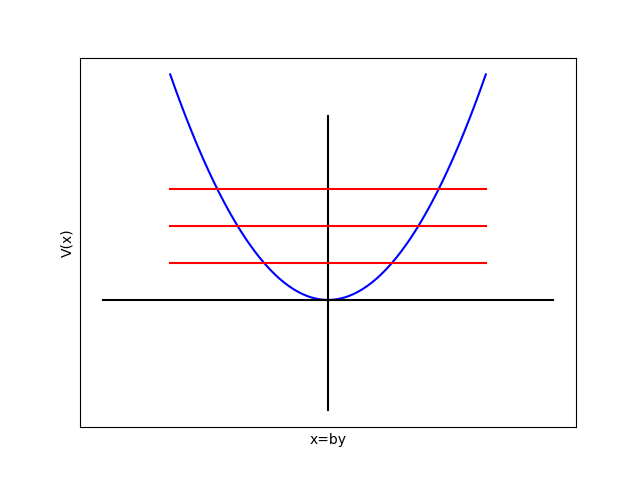
\includegraphics{images7/sol.png}
  \caption{Potential V(x) and some energy levels.}
\end{figure}

We can see the solution for the problem in the figure above, where the distance of the gaps between the energies is always $\hbar\omega$.


\section{Temperature}

We have solved our potential, but we want to think now about a problem wiht multiple of this potentials. Firstly, we assume we are talking about an ideal gas wich means the particles don't talk one with each others. We want to answer the question; At a temperature, T what is the probablity that the energy is $\left(n+\frac{1}{2}\right)\omega$

We want to relate $K_b T <-> \left(n+\frac{1}{2}\right)\omega$. We have Boltzmann equation that say:

\begin{equation}
  P_n = Ne^{\frac{-(n+1/2)\hbar\omega}{k_B T}}
\end{equation}

It is a negative exponential where the fall of depend on T

Because it is a probablity for a fixed N we should have $\sum_{n=0}^{N}P_n = 1$ when N goes to $\infty$.

The average energy, E, will be define as:

\begin{equation}
  E = \sum_{n=0}^{\infty}E_nP_n
\end{equation}

If we called $\beta = \hbar\omega/k_B T$ we can get the average energy as:

\begin{equation}
  \frac{E}{k_B T} = \frac{\beta(1+e^{-\beta})}{2(1-e^{-\beta})}
\end{equation}

The behaviour of this function can be seen in the plot below.


\begin{figure}[H]
  \centering
  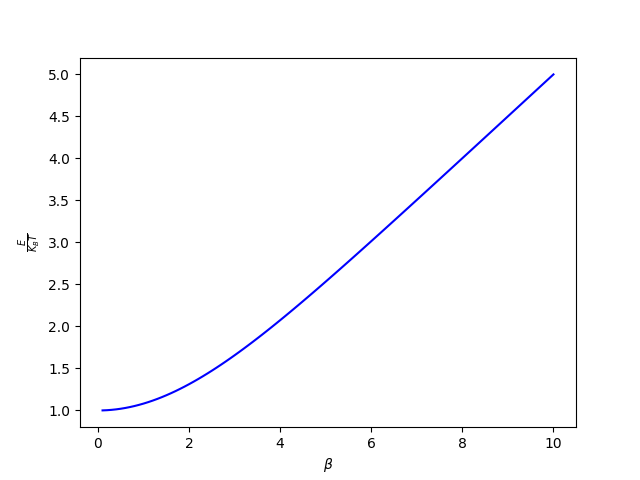
\includegraphics{images7/E_beta.png}
  \caption{Potential V(x) and some energy levels.}
\end{figure}

If T goes to infinite the average energy goes to $E=K_BT$ and if T goes to 0 the average energy goes to $E=\frac{\hbar\omega}{2}$.

We will retur to the topic of temperature in future chapters.


\setchapterpreamble[u]{\margintoc}
\chapter{2-Dimensional Potential}

We will worked with the harmonic oscilator again, but this time in 2 spatial dimensions.

\section{Classical Mechanics}

As we did in chapter 1 we want to understand first the behaviour of the classical mechanics for the problem.

The potential V(x,y) is:

\begin{equation}
  V(x,y) = \frac{1}{2} k (x^2+y^2) = \frac{1}{2} k \rho^2
\end{equation}

The math becomes easier if we used polar coordinates as we did in Chapter 1. In this coordinates the energy is:

\begin{equation}
  E = \frac{1}{2} m \left(\frac{\partial \rho}{\partial t}\right)^2 + \frac{L^2}{2m\rho^2} + \frac{1}{2}k \rho^2
\end{equation}

We are going to solve for the change among time in $\rho$ to solve the problem.

\begin{equation}
  \begin{array}{c}
    \frac{\partial \rho}{\partial t} = \sqrt{\frac{2}{m}\left(E-\frac{L^2}{2 m \rho^2}-\frac{1}{2}k\rho^2\right)}
    \\

    \\
    \frac{\partial \rho}{\partial t} = \sqrt{\frac{k}{m\rho^2}\left(\frac{2E}{k}\rho^2-\frac{L^2}{m k}-\rho^4\right)}
  \end{array}
\end{equation}

Using equation 7.2 we can turn the previous equation into:

\begin{equation}
  \begin{array}{c}
    \frac{\rho}{\omega}\frac{\partial \rho}{\partial t} = \sqrt{\frac{2E}{m^2\omega^2}\rho^2 - \frac{L^2}{m \omega^2}-\rho^4}
  \end{array}
\end{equation}

We are going to change the variable $\rho$ to $u$, where $u=\rho^2$. Solving for u the equation turns into:

\begin{equation}
  \begin{array}{c}
    \frac{1}{2\omega}\frac{\partial u}{\partial t} = \sqrt{- \frac{L^2}{m \omega^2}+ \frac{2E}{m^2\omega^2}u -u^2}
    \\

    \\
    \frac{1}{2\omega}\frac{\partial u}{\partial t} = \sqrt{\left(\frac{E^2}{m^2\omega^4} - \frac{L^2}{m^2\omega^2}\right)-\left(u-\frac{E}{m\omega}\right)^2}
    \\

    \\
    \frac{1}{2\omega}\frac{\partial u}{\partial t} = \sqrt{\frac{1}{m^2\omega^4}\left(E^2-L^2\omega^2\right)-\left(u-\frac{E}{m\omega^2}\right)^2}
  \end{array}
\end{equation}

The function inside of the square root needs to be positive, which make us say than the left parenthesis is greater than the right one that is always greater than 0, i. e. :

\begin{equation}
  \begin{array}{c}
    (E^2-L\omega^2) \geq 0
    \\

    \\
    E \geq L\omega
  \end{array}
\end{equation}

We know now that there is a minimum energy, which energy is $E=L\omega$. Whenthe energy is at it's minimum is easy to get u(t):

\begin{equation}
  \begin{array}{c}
    u(t) = \frac{E}{m\omega^2} = constant
    \\

    \\
    \frac{\partial u}{\partial t} = 0
  \end{array}
\end{equation}

To analize the rest of the solution for the Energy we are going to change some of the variables by some unitless variables.

\begin{equation}
  \label{8.8}
  \begin{array}{c}
    E = \alpha L \omega
    \\

    \\
    u = \beta \frac{E}{m\omega^2}
    \\

    \\
    \omega t = \tau
  \end{array}
\end{equation}

From the previous analysis of the minimum energy we can say that $\alpha \geq 1$. Now that we have our new parameters well define we can rewrite the expression we have been working with.

\begin{equation}
  \begin{array}{c}
    \frac{\alpha L}{m\omega}\frac{1}{2} \frac{\partial \beta}{\partial \tau} = \sqrt{\frac{L^2\omega^2}{m^2\omega^4}[\alpha^2-1]-\frac{\alpha^2 L^2}{m^2\omega^2}[\beta-1]^2}
    \\

    \\
    \frac{1}{2} \frac{\partial \beta}{\partial \tau} = \sqrt{\left(1-\frac{1}{\alpha^2}\right)-(\beta-1)^2}
  \end{array}
\end{equation}

Knowing that alpha is a fixed constant we can solve this equation. But first i will make the math simpler by saying $A = \left(1-\frac{1}{\alpha^2}\right)$

\begin{equation}
  \begin{array}{c}
    \frac{\partial \beta}{2\sqrt{A-(\beta-1)^2}} = \partial\tau
  \end{array}
\end{equation}

To solve the integral we have to define the limits; for $\tau$ as it is a measure of time is going to start at $\tau=0$ and end in a general $\tau$, but for $\beta$ it can start at any arbitrary $\beta \geq 0$, so we will say that $\beta$ goes from $\beta_0$ to a general $\beta$.

\begin{equation}
  \begin{array}{c}
    \int_{\beta_0}^{\beta}\frac{\partial \beta'}{2\sqrt{A-(\beta-1)^2}} = \int_{0}^{\tau}\partial\tau'
  \end{array}
\end{equation}

This integral can be solved directly if we change the variable beta and the constant A by $f = \beta-1$ and $A = B^2$.

\begin{equation}
  \begin{array}{c}
    \int_{f_0+1}^{f+1}\frac{\partial f'}{2\sqrt{A-f'^2}} = \int_{0}^{\tau}\partial\tau'
    \\

    \\
    \int_{f_0+1}^{f+1}\frac{\partial f'}{2\sqrt{A(1-\frac{f'^2}{A}}} = \int_{0}^{\tau}\partial\tau'
    \\

    \\
    \int_{f_0+1}^{f+1}\frac{B \partial f'}{2\sqrt{(1-\frac{f'^2}{B^2}}} = \int_{0}^{\tau}\partial\tau'
  \end{array}
\end{equation}

This last integral can be solved directly and it will give us the result for $f(\tau)$ and then we can recover the solution for $\beta(\tau)$.

\begin{equation}
  \begin{array}{c}
    \arcsin(\frac{f+1}{B}) - \arcsin(\frac{f_0}{B}) =2\tau
    \\

    \\
    \beta(\tau) = B \sin\left(2\tau + \arcsin\left(\frac{\beta_0}{B}\right) \right)
    \\

    \\
    \beta(\tau) = \sqrt{1-\frac{1}{\alpha^2}} \sin\left(2\tau + \arcsin\left(\frac{\beta_0}{\sqrt{1-\frac{1}{\alpha^2}}}\right) \right)
  \end{array}
\end{equation}

This is our final solution for $\beta$, from this solution we can get $\rho(t)$ by undoing the changes of variables in \ref{8.8}.

\begin{marginfigure}[-2cm]
  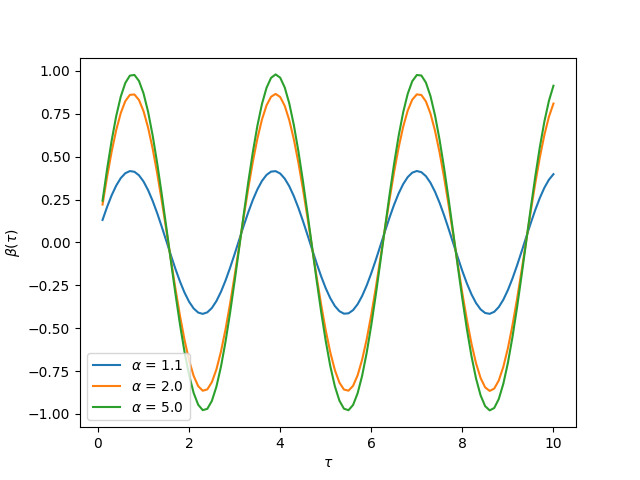
\includegraphics{images8/beta_tau.png}
  \caption{$\beta(\tau)$ function for different values of alpha}
  \labfig{beta_tau}
\end{marginfigure}

We can not forget about the other variable, the angle $\phi$. To solve for phi we will used the definition of the angular momentum.

\begin{equation}
  \begin{array}{c}
    L = m \rho^2 \frac{\partial \phi}{\partial t}
    \\

    \\
    \frac{\partial \phi}{\partial t} = \frac{L}{m \rho^2}
    \\

    \\
    \frac{\partial \phi}{\partial \tau} = \frac{1}{\alpha \beta(\tau)}
  \end{array}
\end{equation}

We want to find the solution for $\beta (\phi)$.

\begin{equation}
  \begin{array}{c}
    \frac{\partial\beta}{\partial\phi} = \frac{\frac{\partial\beta}{\partial\tau}}{\frac{\partial\phi}{\partial\tau}} = 2\alpha\beta\sqrt{\left(1-\frac{1}{\alpha^2}-(\beta-1)^2\right)}
  \end{array}
\end{equation}

Solving this equation we end up with:

\begin{equation}
  \begin{array}{c}
    \beta(\phi) = 1+\sqrt{\left(1-\frac{1}{\alpha^2}\right)} \sin\left(\frac{1}{\alpha}\tan(\phi)\right)
  \end{array}
\end{equation}

We can turn beta into rho by undoing the changes of variables in \ref{8.8}.

\begin{equation}
    \rho(\phi) = \sqrt{\beta(\phi)\frac{E}{m\omega^2}} = \sqrt{\beta(\phi)\alpha \r}
\end{equation}

In the figure below we can see the orbital movement of the particle for different values of $\alpha$.

\begin{figure}
  \centering
  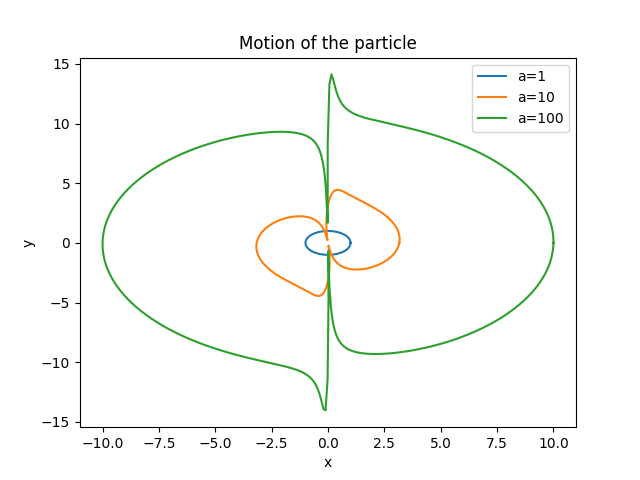
\includegraphics{images8/beta_theta.png}
  \caption{Orbital movement of the particle for different values of $\alpha$}
\end{figure}

\section{Quantum Mechanics}

We are going to solve the problem using the Schrödinger wave equation.

\begin{equation}
  \begin{array}{c}
    -\frac{\hbar^2}{2m} \left[\frac{\partial^2\phi}{\partial x^2} + \frac{\partial^2\phi}{\partial y^2}\right] + \frac{1}{2} m \omega^2 (x^2+y^2)\phi = E \phi
  \end{array}
\end{equation}

In this case we are not going to solve the problem in polar coordinates, we are going to solve it in cartesian coordinates. First, we have to set the equation to natural units.

\begin{equation}
  \begin{array}{c}
    x = b u
    \\

    \\
    y = b v
    \\

    \\
    b^2 = \frac{\hbar}{m\omega}
    \\

    \\
    \phi(x=bu,y=bv) = \psi(u,v)
  \end{array}
\end{equation}

Our wave equation now is:

\begin{equation}
  \begin{array}{c}
    -\frac{1}{2}\hbar\omega \left[\frac{\partial^2\psi}{\partial u^2} + \frac{\partial^2\psi}{\partial v^2}\right] + \frac{1}{2} \hbar \omega (u^2+v^2)\psi = E \psi
  \end{array}
\end{equation}

As we did in the classical aproach we are going to change the energy by $E=\alpha\hbar\omega$. The wave equation now looks like:

\begin{equation}
  \begin{array}{c}
    \left[-\frac{1}{2}\left(\frac{\partial^2}{\partial u^2}+\frac{\partial^2}{\partial v^2}\right)+\frac{1}{2}(u^2+v^2)\right]\psi = \alpha \psi
  \end{array}
\end{equation}

As we did in one dimension we can use some operators to solve this equation. We are going to define this as:

\begin{equation}
  \begin{array}{c}
    a_u = \frac{1}{\sqrt{2}}\left[\frac{\partial}{\partial u}+u\right]
    \\

    \\
    a_v = \frac{1}{\sqrt{2}}\left[\frac{\partial}{\partial v}+v\right]
    \\

    \\
    a_u^{\dagger} = \frac{1}{\sqrt{2}}\left[-\frac{\partial}{\partial u}+u\right]
    \\

    \\
    a_v^{\dagger} = \frac{1}{\sqrt{2}}\left[-\frac{\partial}{\partial v}+v\right]
  \end{array}
\end{equation}

It can be proved that $a a^{\dagger}$ is an hermitian operator of $\chi$ for any of the variables; u,v.

We have also similar relations to the ones we had in one dimension.

\begin{equation}
  \begin{array}{c}
    \left[a_u,a_u^{\dagger}\right] = 1
    \\

    \\
    \left[a_v,a_v^{\dagger}\right] = 1
    \\

    \\
    \left[a_u,a_v\right] = 0
    \\

    \\
    \left[a_u^{\dagger},a_v^{\dagger}\right] = 0
    \\

    \\
    N_u = a_u^{\dagger}a_u
    \\

    \\
    N_v = a_v^{\dagger}a_v
    \\

    \\
    \left[N_u,a_u^{\dagger}\right] = a_u^{\dagger}
    \\

    \\
    \left[N_u,a_u\right] = -a_u
    \\

    \\
    \left[N_v,a_v^{\dagger}\right] = a_v^{\dagger}
    \\

    \\
    \left[N_v,a_v\right] = -a_v
  \end{array}
\end{equation}

The commutator of any two cross operators is 0. With this we end up with the following equation:

\begin{equation}
  \begin{array}{c}
    \left[N_u+N_v\right] \psi = (\alpha-1) \psi
  \end{array}
\end{equation}

Which means that $\alpha \geq 1$, as it was in classical mechanics. We can use the operators $a_u^{\dagger}$ or $a_v^{\dagger}$ to get the next level of energy for the equation.

\begin{equation}
  \begin{array}{c}
      \left[N_u+N_v+1\right] (a^{\dagger}\psi) = \left[a^{\dagger}N_u + a^{\dagger} + a^{\dagger}N_v \right]
      \\

      \\
      \left[N_u+N_v+1\right] (a^{\dagger}\psi) = a^{\dagger}[N_u+N_v+1]\psi
      \\

      \\
      \left[N_u+N_v+1\right] (a^{\dagger}\psi) = (\alpha+1-1)a^{\dagger}\psi
  \end{array}
\end{equation}

The operator $a^{\dagger}$ could be either of the two posible operators, and the result is the same. We can say that the operator $a^{\dagger}$ is giving us the next level of energy for the equation, $\alpha$ increases by one.

There is an $\alpha = 1$, which is the minimum energy for the system, which means that there is a lower energy state $\psi_0$ where:

\begin{equation}
  \begin{array}{c}
    \left[N_u+N_v\right] \psi_0(u,v) = 0
  \end{array}
\end{equation}

So:

\begin{equation}
  \begin{array}{c}
    a_u \psi_0(u,v) = 0
    a_v \psi_0(u,v) = 0
  \end{array}
\end{equation}

There must be a function $\psi_0(u,v)$ that satisfies this two equations. Let's try to solve it.

\begin{equation}
  \begin{array}{c}
    \left(\frac{\partial}{\partial u} + u\right)\psi_0(u,v) = 0
    \\

    \\
    \left(\frac{\partial}{\partial v} + v\right)\psi_0(u,v) = 0
  \end{array}
\end{equation}

The solution for this equation is:

\begin{equation}
  \begin{array}{c}
    \ln\psi_0(u,v) + \frac{1}{2}u^2 = f(v)
    \\

    \\
    \ln\psi_0(u,v) + \frac{1}{2}v^2 = f(u)
    \\

    \\
    \psi_0(u,v) = A e^{-\frac{1}{2}(u^2+v^2)}
  \end{array}
\end{equation}

Where A is the normalization factor than can be calculated by:

\begin{equation}
  \begin{array}{c}
    \int_{-\infty}^{\infty}\int_{-\infty}^{\infty} \psi_0^2(u,v) du dv = 1
    \\

    \\
    \int_{-\infty}^{\infty}\int_{-\infty}^{\infty} A^2 e^{-u^2-v^2} du dv = 1
    \\

    \\
    A^2 \int_{-\infty}^{\infty} e^{-u^2} du \int_{-\infty}^{\infty} e^{-v^2} dv = 1
    \\

    \\
    A^2 \left(\sqrt{\pi}\right)^2 = 1
    \\

    \\
    A = \frac{1}{\sqrt{\pi}}
  \end{array}
\end{equation}

This is the solution for the ground state of the system. We can now use the operator $a^{\dagger}$ to get the next level of energy even for u or for v, both states will have the same energy but different functions, i.e. $\alpha=2$ have two states $\psi_{1,0}$ and $\psi_{0,1}$.

\begin{equation}
  \begin{array}{c}
    \psi_0 = \frac{1}{\sqrt{\pi}} e^{-\frac{1}{2}(u^2+v^2)}
    \\

    \\
    \psi_{1,0} = A_{1,0} a_u^{\dagger} \psi_0 = A_{1,0} \frac{1}{\sqrt{2}}\left[-\frac{\partial}{\partial u}+u\right]\psi_0 = A_{1,0} \sqrt{\frac{2}{\pi}} u e^{-\frac{u^2+v^2}{2}}
    \\

    \\
    \psi_{0,1} = A_{0,1} a_v^{\dagger} \psi_0 = A_{0,1} \frac{1}{\sqrt{2}}\left[-\frac{\partial}{\partial v}+v\right]\psi_0 = A_{0,1} \sqrt{\frac{2}{\pi}} v e^{-\frac{u^2+v^2}{2}}
  \end{array}
\end{equation}

To determine the normalization coeficient we have to use the same procedure as before.

\begin{equation}
  \begin{array}{c}
    A^2_{1,0} = \int_{-\infty}^{\infty}\int_{-\infty}^{\infty} \psi_{1,0}^2(u,v) du dv = \frac{2}{\pi} \int_{-\infty}^{\infty}\int_{-\infty}^{\infty} u^2 e^{-(u^2+v^2)} du dv
  \end{array}
\end{equation}

To solve this integral we are going to use polar coordinates.

\begin{equation}
  \begin{array}{c}
    A^2_{1,0} = \frac{2}{\pi} \int_{0}^{\infty} rdr \int_{0}^{2\pi} r^2 \sin^2(\theta) e^{-r^2} d\theta =
    \\

    \\
    = \frac{2}{\pi} \int_{0}^{\infty} r^3 e^{-r^2} dr \int_{0}^{2\pi} \sin^2(\theta) d\theta = \frac{2}{\pi} \frac{1}{2} \pi = 1
  \end{array}
\end{equation}

Which means that $A^2 = 1$, so $A = e^{i\phi}$, but we are only interested in the real part of the function, so $A = 1$. We can do the same for $\psi_{0,1}$.

\marginnote{This variables are called Hidden Variables in quantum mechanics. They are not observable, but they have become important for new physics, for example in the field of quantum computation.}

We can continue this process to get the next levels of energy. The final results fo the next level are:

\begin{equation}
  \begin{array}{c}
    \psi_{2,0} = \frac{2u^2-1}{2\sqrt{\pi}}e^{-\frac{u^2+v^2}{2}}
    \\

    \\
    \psi_{0,2} = \frac{2v^2-1}{2\sqrt{\pi}}e^{-\frac{u^2+v^2}{2}}
    \\

    \\
    \psi_{1,1} = \frac{uv}{\sqrt{2\pi}}e^{-\frac{u^2+v^2}{2}}
  \end{array}
\end{equation}

The solutions can be visualized in the following figures.

\begin{figure}
  \centering
  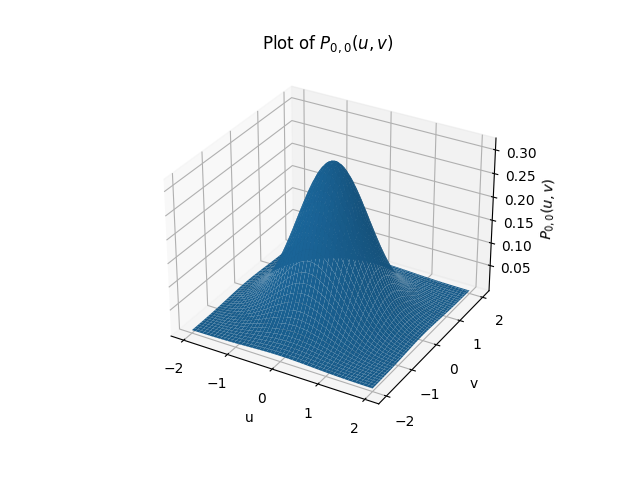
\includegraphics{images8/P_0,0.png}
  \caption{Probability distribution for the state $\psi_{0,0}(u,v)$}
\end{figure}

\begin{figure}
  \centering
  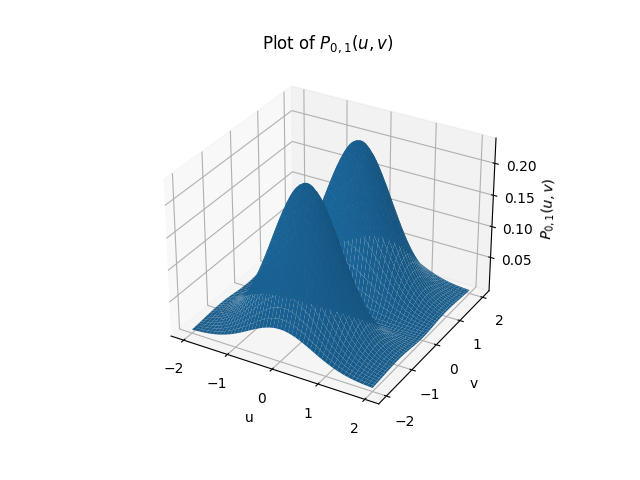
\includegraphics{images8/P_0,1.png}
  \caption{Probability distribution for the state $\psi_{0,1}(u,v)$}
\end{figure}

\begin{figure}
  \centering
  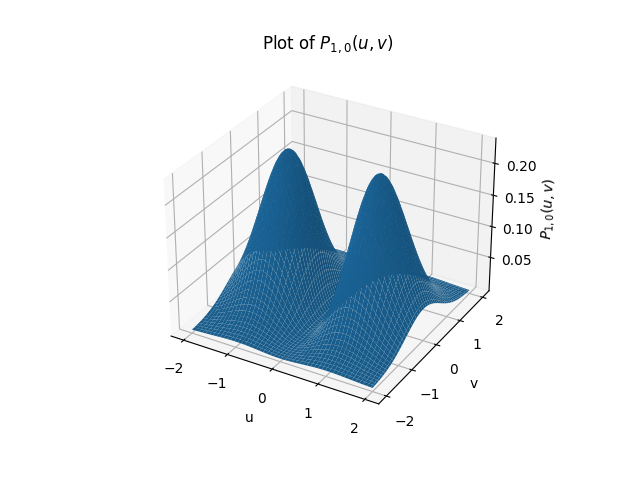
\includegraphics{images8/P_1,0.png}
  \caption{Probability distribution for the state $\psi_{1,0}(u,v)$}
\end{figure}

\begin{figure}
  \centering
  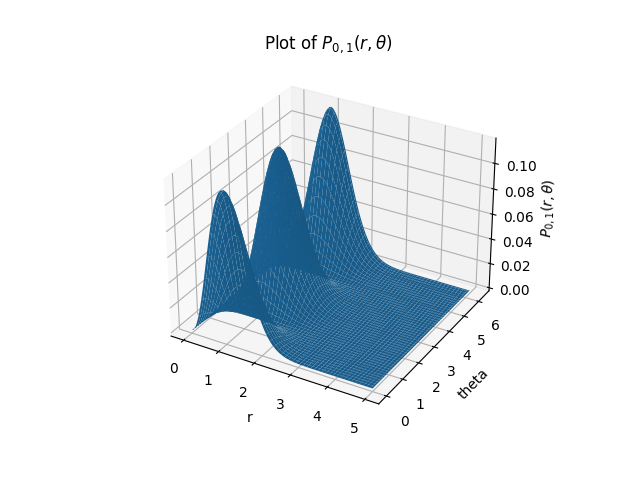
\includegraphics{images8/P_0,1(r).png}
  \caption{Probability distribution for the state $\psi_{0,1}(r,\theta)$}
\end{figure}

\begin{figure}
  \centering
  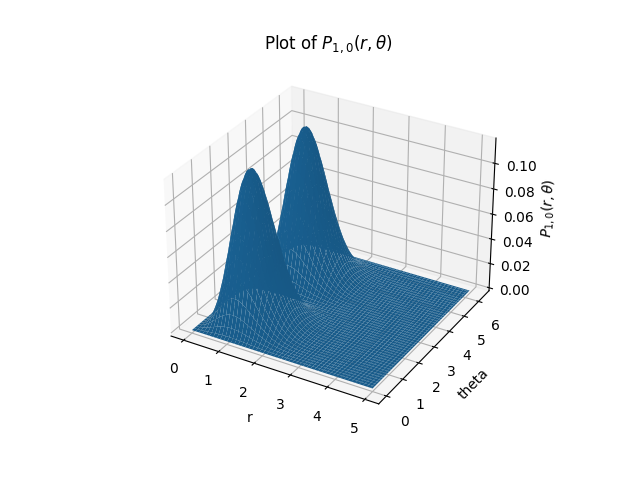
\includegraphics{images8/P_1,0(r).png}
  \caption{Probability distribution for the state $\psi_{1,0}(r,\theta)$}
\end{figure}

\section{Mixed Quantum states}

Given $\alpha = 2$ and the density Probability of a mixed state $\psi$, we can say that:

\begin{equation}
  \psi = C_{1,0} \psi_{1,0} + C_{0,1} \psi_{0,1}
\end{equation}

Where $C_{1,0}$ and $C_{0,1}$ are real numbers, (to keep it simpler). If the probability density is normalized we found:

\begin{equation}
  \begin{array}{c}
    \int_{-\infty}^{\infty} \int_{-\infty}^{\infty} \psi^{\star}(u,v)\psi(u,v) du dv = 1
    \\

    \\
    \int_{-\infty}^{\infty} \int_{-\infty}^{\infty} \left(C_{1,0} \psi_{1,0} + C_{0,1} \psi_{0,1}\right)^{\star} \left(C_{1,0} \psi{1,0} + C_{0,1} \psi{0,1}\right) du dv = 1
    \\

    \\
    \int_{-\infty}^{\infty} \int_{-\infty}^{\infty} \left(C_{1,0}^2 \psi^*_{1,0} \psi{1,0} + C_{0,1}^2 \psi^*_{0,1} \psi{0,1}\right) du dv = 1
    \\

    \\
    C_{1,0}^2 + C_{0,1}^2 = 1
  \end{array}
\end{equation}

This means that the sum of the square of the coefficients is going to be 1.

We can transform the probability into any system, we are going to choose the probability in terms of $r$ and $\theta$

\begin{equation}
  \begin{array}{c}
    P(r,\theta) = \psi^{\star}(r,\theta)\psi(r,\theta) = \left(C_{1,0} \psi^*_{1,0} + C_{0,1} \psi^*_{0,1}\right)^{\star} \left(C_{1,0} \psi{1,0} + C_{0,1} \psi{0,1}\right)
    \\

    \\
    P(r,\theta) = \frac{2}{\pi} \left(C_{1,0}^2\sin^2\theta + 2C_{1,0}C_{0,1} \sin\theta \cos\theta + C_{0,1}\cos^2\theta \right)
    \\

    \\
    P(r,\theta) = \frac{2}{\pi} \left(\frac{1}{2}+\frac{C_{0,1}^2-C_{1,0}^2}{2}\cos 2\theta + C_{1,0}C_{0,1} \sin 2\theta \right)
\end{array}
\end{equation}

This means than knowing the probability depending on the angle $\theta$ we can get the coefficients $C_{1,0}$ and $C_{0,1}$, i.e. how the state is distributed in terms of the pure quantum states.

\section{The angular momentum}

As we did in the classical mechanics we are going to solve the problem in polar coordinates.

We need to transform the variables and derivatives into a polar system.

\begin{equation}
  \begin{array}{cc}
    u = r \cos\theta & v = r \sin\theta
    \\

    \\
    du = (dr) \cos\theta - r \sin\theta d\theta & dv = (dr) \sin\theta + r \cos\theta d\theta
  \end{array}
\end{equation}

We will rename $\psi(u,v)$ to $\chi(r,\theta)$ and we want to know how the derivatives behave for $\chi$.

\begin{equation}
  \begin{array}{c}
    \frac{\partial}{\partial u} \chi= \left[\left(\frac{\partial}{\partial\theta}\right)_{r} \left(\frac{\partial \theta}{\partial u}\right)_v +\left(\frac{\partial}{\partial r}\right)_\theta \left(\frac{\partial r}{\partial u}\right)_v \right] \chi =
    \\

    \\
    = \left(\frac{-\sin\theta}{r}\frac{\partial}{\partial \theta} + \cos\theta\frac{\partial}{\partial r} \right) \chi
    \\

    \\
    \frac{\partial}{\partial v} \chi= \left[\left(\frac{\partial}{\partial\theta}\right)_{r} \left(\frac{\partial \theta}{\partial v}\right)_u +\left(\frac{\partial}{\partial r}\right)_\theta \left(\frac{\partial r}{\partial v}\right)_u \right] \chi =
    \\

    \\
    = \left(\frac{\cos\theta}{r}\frac{\partial}{\partial \theta} + \sin\theta\frac{\partial}{\partial r} \right) \chi
  \end{array}
\end{equation}

We need to the second derivative.

\begin{equation}
  \begin{array}{c}
    \frac{\partial^2}{\partial u^2} \chi = \left(\frac{-\sin\theta}{r}\frac{\partial}{\partial \theta} + \cos\theta\frac{\partial}{\partial r} \right) \left(\frac{-\sin\theta}{r}\frac{\partial}{\partial \theta} + \cos\theta\frac{\partial}{\partial r} \right) \chi =
    \\

    \\
    = \left(\frac{\sin^2\theta}{r^2}\frac{\partial^2}{\partial\theta^2} + \frac{\sin^2\theta}{r}\frac{\partial}{\partial r} + \cos^2\theta \frac{\partial^2}{\partial r^2} \right) \chi
    \\

    \\
    \frac{\partial^2}{\partial v^2} \chi = \left(\frac{\cos\theta}{r}\frac{\partial}{\partial \theta} + \sin\theta\frac{\partial}{\partial r} \right) \left(\frac{\cos\theta}{r}\frac{\partial}{\partial \theta} + \sin\theta\frac{\partial}{\partial r} \right) \chi =
    \\

    \\
    = \left(\frac{\cos^2\theta}{r^2}\frac{\partial^2}{\partial\theta^2} + \frac{\cos^2\theta}{r}\frac{\partial}{\partial r} + \sin^2\theta \frac{\partial^2}{\partial r^2} \right) \chi
  \end{array}
\end{equation}

Our wave equation now looks like:

\begin{equation}
  \begin{array}{c}
    \left[-\frac{1}{2}\left(\frac{\partial^2}{\partial r^2}+\frac{1}{r}\frac{\partial}{\partial r}+\frac{1}{r^2}\frac{\partial^2}{\partial\theta^2}\right)+\frac{1}{2}r^2\right]\chi = \alpha \chi
  \end{array}
\end{equation}

If we compare this equation with the one we had for classical mechanics we can see a relation between the different energies in classical mechanics and these terms.

\begin{itemize}
  \item $\frac{1}{2}\left(\frac{\partial^2}{\partial r^2}+\frac{1}{r}\frac{\partial}{\partial r}\right)$ is the kinetic energy in the radial direction.
  \item $\frac{1}{2}\frac{1}{r^2}\frac{\partial^2}{\partial\theta^2}$ is the angular kinetic energy.
  \item $\frac{1}{2}r^2$ is the potential energy.
\end{itemize}

As we did in classical mechanics we are going to define the angular momentum as the operator: $L_z = \frac{\partial}{\partial\theta}$.

We want to know how this operator behaves with the operator $H$ and the wave function.

\begin{equation}
  \begin{array}{c}
    (H L_z) \chi = \frac{-1}{2} \frac{\partial^3\chi}{\partial r^2 \partial\theta} - \frac{1}{2r} \frac{\partial^2\chi}{\partial r \partial\theta} + \frac{1}{2r^2} \frac{\partial^3\chi}{\partial\theta^3} + \frac{1}{2} r^2 \frac{\partial\chi}{\partial\theta}
    \\

    \\
    (L_z H) \chi = \frac{-1}{2} \frac{\partial^3\chi}{\partial r^2 \partial\theta} - \frac{1}{2r} \frac{\partial^2\chi}{\partial r \partial\theta} + \frac{1}{2r^2} \frac{\partial^3\chi}{\partial\theta^3} + \frac{1}{2} r^2 \frac{\partial\chi}{\partial\theta}
  \end{array}
\end{equation}

As we can see both operations are the same, this proves that the two operators commute.

\begin{equation}
  \begin{array}{c}
    [H,L_z] = 0
  \end{array}
\end{equation}

If $H\chi = \alpha \chi$:

\begin{equation}
  \begin{array}{c}
    H(L_z\chi) = L_z(H\chi) = \alpha(L_z\chi)
  \end{array}
\end{equation}

Wich means that $L_z\chi$ is an eigenvector of the operator $H$ with the same eigenvalue $\alpha$. The eigenspace can be defined by eigenvectors of $H$ and by eigenvectors of $H$ and $L_z$ at the same time.

We can found now the eigenvectors of $L_z$.

\begin{equation}
  L_z \chi = l \chi
\end{equation}

The solution for this differential equation is:

\begin{equation}
  \begin{array}{c}
    \chi = R(r) e^{l\theta}
  \end{array}
\end{equation}

Because the function $\chi$ is periodic in $\theta$ we can say that $l=i m$.

\begin{equation}
  \begin{array}{c}
    \chi = R(r) e^{i m \theta}
  \end{array}
\end{equation}

We didn't assume anything, we proved that because the operator commute the function can be described as above. This two operators commute because the force is a central force wich means that $V(r)$ is only a function of $r$.

\begin{equation}
  \begin{array}{c}
    H \chi_{\alpha,m} = \alpha \chi_{\alpha,m}
    \\

    \\
    L_z \chi_{\alpha,m} = i m \chi_{\alpha,m}
  \end{array}
\end{equation}

Now we have to solve the wave equation for the radial function, $R(r)$.

\begin{equation}
  \label{8.49}
  \begin{array}{c}
    \left[\frac{d^2}{dr^2}+\frac{1}{r}\frac{d}{dr}-\frac{m^2}{r^2}-r^2+2\alpha\right]R(r) = 0
  \end{array}
\end{equation}

If we look at the results in Section 3, we can see that there is an exponential factor in the solution. We will take that out to make math simpler.

\begin{equation}
  \begin{array}{c}
    R(r) = e^{-\frac{r^2}{2}} P(r)
    \\

    \\
    \frac{dR}{dr} = \left(\frac{dP}{dr}-rP \right)e^{\frac{-r^2}{2}}
    \\

    \\
    \frac{d^2R}{dr^2} = \left(\frac{d^2P}{dr^2}-2r\frac{dP}{dr}+(r^2-1)P \right)e^{\frac{-r^2}{2}}
  \end{array}
\end{equation}

If we substitute this into \ref{8.49}:

\begin{equation}
  \begin{array}{c}
    \left[\frac{d^2P}{dr^2}- 2r\frac{dP}{dr} + (r^2-1)P +\frac{1}{r}\frac{dP}{dr}-P-\frac{m^2P}{r^2}-r^2P+2\alpha P\right]e^{\frac{-r^2}{2}} = 0
    \\

    \\
    \frac{d^2P}{dr^2} + \left(\frac{1}{r}-2r\right)\frac{dP}{dr}+\left(2\alpha-2-\frac{m^2}{r^2}\right)P = 0
  \end{array}
\end{equation}



We expect P(r) to be a polinomic function, but for a polinome to be normalizable must be finite wich means having a finite number of terms. Let's assume $P(r) ~ r^\beta$ for $r\to 0$. Near $r=0$ the derivatives will be:

\begin{equation}
  \begin{array}{c}
    \frac{dP}{dr} ~ r^{\beta-1}
    \\

    \\
    \frac{d^2P}{dr^2} ~ r^{\beta-2}
  \end{array}
\end{equation}

If we substitute this into the equation we get:

\begin{equation}
  \begin{array}{c}
    \beta(\beta-1)r^{\beta-2}+ \left(\frac{1}{r}-2r\right)\beta r^{\beta-1} + (2\alpha-2-\frac{m^2}{r^2})r^\beta = 0
    \\

    \\
    \left[\beta(\beta-1)+\beta-m^2\right]r^{\beta-2}+(2\alpha-2-2\beta)r^\beta = 0
    \\

    \\
    \beta(\beta-1)+\beta-m^2 = 0 \Rightarrow \beta = \beta^2 = m^2 \Rightarrow \beta = |m|
  \end{array}
\end{equation}

$\beta$ has to be positive. We can redefine $P(r)$ as:

\begin{equation}
  \begin{array}{c}
    P(r) = r^{|m|} U(r)
    \\

    \\
    \frac{d P}{dr} = |m| r^{|m|-1} U(r) + r^{|m|} \frac{dU}{dr}
    \\

    \\
    \frac{d^2 P}{dr^2} = |m| (|m|-1) r^{|m|-2} U(r) + 2 |m| r^{|m|-1} \frac{dU}{dr} + r^{|m|} \frac{d^2U}{dr^2}
    \\

    \\
    \left(\frac{1}{r}-2r\right) \frac{dP}{dr} = |m|r^{|m|-2} U(r) - 2 |m| r^{|m|-1} \frac{dU}{dr} - 2 r^{|m|+1} \frac{dU}{dr}
    \\

    \\
    \left(2\alpha-2-\frac{m^2}{r^2}\right)P = (2\alpha-2) r^{|m|} U(r) - m^2 r^{|m|-2} U(r)
  \end{array}
\end{equation}

If we substitute this into the differential equation we get:

\begin{equation}
  \begin{array}{c}
    (2\alpha-2-2|m|) r^{|m|}U(r) + \left[(2|m|+1)r^{|m|-1}-2r^{|m|+1}\right]\frac{dU}{dr} +r^{|m|} \frac{d^2U}{dr^2} = 0
    \\

    \\
    \frac{d^2U}{dr^2}+ \left(\frac{2|m|+1}{r}-2r\right)\frac{dU}{dr} + 2(\alpha-1-|m|) U = 0
  \end{array}
\end{equation}

This differential equation can be solved using Frobenius Method. We are going to assume that U(r) is an "infinite" polinomic function.

\begin{equation}
  \begin{array}{c}
  U(r) = \sum_{n=0}^{\infty} u_n r^n
  \\

  \\
  \frac{dU}{dr} = \sum_{n=0}^{\infty} n u_n r^{n-1}
  \\

  \\
  \frac{d^2U}{dr^2} = \sum_{n=0}^{\infty} n(n-1) u_n r^{n-2}
  \\

  \\
  \left(\frac{2|m|+1}{r}-2r\right)\frac{dU}{dr} = \frac{(2|m|+1)u_1}{r} + \sum_{0}^{\infty} (2|m|+1)u_{n+2}(n+2)r^n - \sum_{0}^{\infty} 2 u_n n r^n
  \\

  \\
  2(\alpha-1-|m|) U = \sum_{0}^{\infty} 2(\alpha-1-|m|)  u_n r^n
  \end{array}
\end{equation}

Substituying:

\begin{equation}
  \begin{array}{c}
    0 = \frac{2|m|+1}{r}u_1 + \sum_{0}^{\infty} \left[u_{n+2}\left((n+2)(2|m|+1)+(n+2)(n+1)\right)+u_n\left(\2(\alpha-1-|m|)-2n\right)\right]r^n
  \end{array}
\end{equation}

This has to be 0 for every r, but also the first term has to be null, for the function to exist in $r=0$.

\begin{equation}
  \begin{array}{c}
    u_1 = 0
    \\

    \\
    u_{n+2}\left[(n+2)(2|m|+1)+(n+2)(n+1)\right]+u_n\left[\2(\alpha-1-|m|)-2n\right] = 0
    \\

    \\
    u_{n+2} = \frac{2[1+|m|+n-\alpha]}{(n+2)(2|m|+n+2)}u_n ; n\geq0
  \end{array}
\end{equation}

All the odd terms are going to be 0. We need this to be finite so we have to arrange a value N for when all the greater terms are 0, i.e. $u_{N+2} = 0$. This implies:

\begin{equation}
  \begin{array}{c}
    2[1+|m|+N-\alpha] = 0 \Rightarrow \alpha= 1+|m|+N
  \end{array}
\end{equation}

We know that N has to be even. We can represent alpha with this new parameters N and m.

\begin{tabular}{| c | c | c | c |}
  \hline
  $N$ & $m$ & $\alpha$ & $\chi(r,\theta)$ \\
  \hline
  0 & 0 & 1  & $\chi(r,\theta) = u_0 e^{\frac{-r^2}{2}}$              \\
  \hline
  0 & +1 & 2 & $\chi(r,\theta) = u_0re^{\frac{-r^2}{2}}e^{i\theta}$   \\
  \hline
  0 & -1 & 2 & $\chi(r,\theta) = u_0 re^{\frac{-r^2}{2}}e^{i\theta}$  \\
  \hline
  2 & 0 & 3  & $\chi(r, \theta) = u_0(1-r^2)e^{\frac{-r^2}{2}}$ \\
  \hline
  0 & +2 & 3 & $\chi(r, \theta) = u_0r^2e^{\frac{-r^2}{2}}e^{2i\theta}$ \\
  \hline
  0 & -2 & 3 & $\chi(r, \theta) = u_0r^2e^{\frac{-r^2}{2}}e^{2i\theta}$ \\
  \hline
\end{tabular}

This gave us pretty much every understandment on harmonic oscilators. We will get more into the angular momentum in the next chapter.



% \setchapterstyle{kao}
% \setchapterpreamble[u]{\margintoc}
% \chapter{Mathematics and Boxes}
% \labch{mathematics}

% \section{Theorems}

% Despite most people complain at the sight of a book full of equations,
% mathematics is an important part of many books. Here, we shall
% illustrate some of the possibilities. We believe that theorems,
% definitions, remarks and examples should be emphasised with a shaded
% background; however, the colour should not be to heavy on the eyes, so
% we have chosen a sort of light yellow.\sidenote{The boxes are all of the
% same colour here, because we did not want our document to look like
% \href{https://en.wikipedia.org/wiki/Harlequin}{Harlequin}.}

% \begin{definition}
% \labdef{openset}
% Let $(X, d)$ be a metric space. A subset $U \subset X$ is an open set
% if, for any $x \in U$ there exists $r > 0$ such that $B(x, r) \subset
% U$. We call the topology associated to d the set $\tau\textsubscript{d}$
% of all the open subsets of $(X, d).$
% \end{definition}

% \refdef{openset} is very important. I am not joking, but I have inserted
% this phrase only to show how to reference definitions. The following
% statement is repeated over and over in different environments.

% \begin{theorem}
% A finite intersection of open sets of (X, d) is an open set of (X, d),
% i.e $\tau\textsubscript{d}$ is closed under finite intersections. Any
% union of open sets of (X, d) is an open set of (X, d).
% \end{theorem}

% \begin{proposition}
% A finite intersection of open sets of (X, d) is an open set of (X, d),
% i.e $\tau\textsubscript{d}$ is closed under finite intersections. Any
% union of open sets of (X, d) is an open set of (X, d).
% \end{proposition}

% \marginnote{You can even insert footnotes inside the theorem
% environments; they will be displayed at the bottom of the box.}

% \begin{lemma}
% A finite intersection\footnote{I'm a footnote} of open sets of (X, d) is
% an open set of (X, d), i.e $\tau\textsubscript{d}$ is closed under
% finite intersections. Any union of open sets of (X, d) is an open set of
% (X, d).
% \end{lemma}

% You can safely ignore the content of the theorems\ldots I assume that if
% you are interested in having theorems in your book, you already know
% something about the classical way to add them. These example should just
% showcase all the things you can do within this class.

% \begin{corollary}[Finite Intersection, Countable Union]
% A finite intersection of open sets of (X, d) is an open set of (X, d),
% i.e $\tau\textsubscript{d}$ is closed under finite intersections. Any
% union of open sets of (X, d) is an open set of (X, d).
% \end{corollary}

% \begin{proof}
% The proof is left to the reader as a trivial exercise. Hint: \blindtext
% \end{proof}

% \begin{definition}
% Let $(X, d)$ be a metric space. A subset $U \subset X$ is an open set
% if, for any $x \in U$ there exists $r > 0$ such that $B(x, r) \subset
% U$. We call the topology associated to d the set $\tau\textsubscript{d}$
% of all the open subsets of $(X, d).$
% \end{definition}

% \marginnote{
% 	Here is a random equation, just because we can:
% 	\begin{equation*}
%   x = a_0 + \cfrac{1}{a_1
%           + \cfrac{1}{a_2
%           + \cfrac{1}{a_3 + \cfrac{1}{a_4} } } }
% 	\end{equation*}
% }

% \begin{example}
% Let $(X, d)$ be a metric space. A subset $U \subset X$ is an open set
% if, for any $x \in U$ there exists $r > 0$ such that $B(x, r) \subset
% U$. We call the topology associated to d the set $\tau\textsubscript{d}$
% of all the open subsets of $(X, d).$
% \end{example}

% \begin{remark}
% Let $(X, d)$ be a metric space. A subset $U \subset X$ is an open set
% if, for any $x \in U$ there exists $r > 0$ such that $B(x, r) \subset
% U$. We call the topology associated to d the set $\tau\textsubscript{d}$
% of all the open subsets of $(X, d).$
% \end{remark}

% As you may have noticed, definitions, example and remarks have
% independent counters; theorems, propositions, lemmas and corollaries
% share the same counter.

% \begin{remark}
% Here is how an integral looks like inline: $\int_{a}^{b} x^2 dx$, and
% here is the same integral displayed in its own paragraph:
% \[\int_{a}^{b} x^2 dx\]
% \end{remark}

% There is also an environment for exercises.

% \begin{exercise}
% Prove (or disprove) the Riemann hypothesis.
% \end{exercise}

% We provide one package for the theorem styles:
% \href{kaotheorems.sty}{kaotheorems.sty}, to which you can pass the
% \Option{framed} option you do want coloured boxes around theorems, like
% in this document.\sidenote{The styles without \Option{framed} are not
% showed, but actually the only difference is that they don't have the
% yellow boxes.} You may want to edit this files according to your taste
% and the general style of the book. However, there is an option to
% customise the background colour of the boxes if you use the
% \Option{framed} option: when you load this package, you can pass it the
% \Option{background=mycolour} option (replace \enquote{mycolour} with the
% actual colour, for instance, \enquote{red!35!white}). This will change
% the colour of all the boxes, but it is also possible to override the
% default colour only for some elements. For instance, the
% \Option{propositionbackground=mycolour} option will change the colour
% for propositions only. There are similar options for theorem,
% definition, lemma, corollary, remark, and example.

% \section[Boxes \& Environments]{Boxes \& Custom Environments
% \sidenote[][*1.8]{Notice that in the table of contents and in the
% 	header, the name of this section is \enquote{Boxes \& Environments};
% 	we achieved this with the optional argument of the \texttt{section}
% 	command.}}

% Say you want to insert a special section, an optional content or just
% something you want to emphasise. We think that nothing works better than
% a box in these cases. We used \Package{mdframed} to construct the ones
% shown below. You can create and modify such environments by editing the
% provided file \href{style/environments.sty}{environments.sty}.

% \begin{kaobox}[frametitle=Title of the box]
% \blindtext
% \end{kaobox}

% If you set up a counter, you can even create your own numbered
% environment.

% \begin{kaocounter}
% 	\blindtext
% \end{kaocounter}

% \section{Experiments}

% It is possible to wrap marginnotes inside boxes, too. Audacious readers
% are encouraged to try their own experiments and let me know the
% outcomes.

% \marginnote[-2.2cm]{
% 	\begin{kaobox}[frametitle=title of margin note]
% 		Margin note inside a kaobox.\\
% 		(Actually, kaobox inside a marginnote!)
% 	\end{kaobox}
% }

% I believe that many other special things are possible with the
% \Class{kaobook} class. During its development, I struggled to keep it as
% flexible as possible, so that new features could be added without too
% great an effort. Therefore, I hope that you can find the optimal way to
% express yourselves in writing a book, report or thesis with this class,
% and I am eager to see the outcomes of any experiment that you may try.

% %\begin{margintable}
% 	%\captionsetup{type=table,position=above}
% 	%\begin{kaobox}
% 		%\caption{caption}
% 		%\begin{tabular}{ |c|c|c|c| }
% 			%\hline
% 			%col1 & col2 & col3 \\
% 			%\hline
% 			%\multirow{3}{4em}{Multiple row} & cell2 & cell3 \\ & cell5
% 			%%& cell6 \\
% 			%& cell8 & cell9 \\
% 			%\hline
% 		%\end{tabular}
% 	%\end{kaobox}
% %\end{margintable}


\setchapterpreamble[u]{\margintoc}
\chapter{3-Dimensional Space}


We've been working with harmonic oscilators and gravitational potentials but there are other interesting potentials that we are going to mention here.

\begin{itemize}
  \item Electric Potential $V(r) = \frac{\alpha}{r}$, $\alpha>0$
  \item Confining Potential $V(r) = k r$
  \item Higgs Potential $V(r) = \frac{\alpha}{r} e^{-mr}$
\end{itemize}

\marginnote[3cm]{There are others like: Reed Potential, Cornell Potential,...}

\section{Angular Momentum in 3 Dimensions}

We can also have potentials that doesn't come from central forces. In those cases we have to look carefully at the angular momentum.

\begin{equation}
  \vec{L} = \vec{r} \times \vec{p}
\end{equation}

\begin{equation}
  \begin{array}{c}
    L_x = y p_z - z p_y\\
    L_y = z p_x - x p_z\\
    L_z = x p_y - y p_x
  \end{array}
\end{equation}

Using our knowledge from equation 2.4 we can say,

\begin{equation}
  \begin{array}{c}
    L_x = -i \hbar (y \frac{\partial}{\partial z} - z \frac{\partial}{\partial y})\\
    L_y = -i \hbar (z \frac{\partial}{\partial x} - x \frac{\partial}{\partial z})\\
    L_z = -i \hbar (x \frac{\partial}{\partial y} - y \frac{\partial}{\partial x})
  \end{array}
\end{equation}

This three components of the angular momentum and the angular momentum itself are hermitian operators. We want to see how they commute between them.

\begin{equation}
  \begin{array}{c}
  (L_xL_y) \psi = -\hbar^2 (y \frac{\partial}{\partial z} - z \frac{\partial}{\partial y})(z \frac{\partial}{\partial x} - x \frac{\partial}{\partial z}) \psi =
  \\

  \\
  = -\hbar^2 \left[y\left(\frac{\partial \psi}{\partial x}+z\frac{\partial^2\psi}{\partial x \partial z}\right)-yx\frac{\partial^2 \psi}{\partial z^2}-z^2 \frac{\partial^2 \psi}{\partial x \partial y}-zx\frac{\partial^2 \psi}{\partial y \partial z}\right] (a)
  \\

  \\
  (L_y L_x) \psi = -\hbar^2 (z \frac{\partial}{\partial x} - x \frac{\partial}{\partial z})(y \frac{\partial}{\partial z} - z \frac{\partial}{\partial y}) \psi =
  \\

  \\
  = -\hbar^2 \left[zy\frac{\partial^2\psi}{\partial x\partial z}-xy\frac{\partial^2\psi}{\partial z^2}-z^2\frac{\partial^2 \psi}{\partial x \partial y}+x\frac{\partial \psi}{\partial y}+xz\frac{\partial^2 \psi}{\partial z \partial y}\right] (b)
  \\

  \\
  (a)-(b) = [L_x,L_y] =i\hbar L_z
  \end{array}
\end{equation}

In the same way it can be prooved that:

\begin{equation}
  \begin{array}{c}
  \left[L_y,L_z\right] =i\hbar L_x
  \\

  \\
  \left[L_z,L_x\right] =i\hbar L_y
  \end{array}
\end{equation}

These 3 operators are closed under conmmutation, wich means that the conmmutation of any two of them give us the third one.

We our going to use the Levi-Civita epsilon to write the angular momentum in a more compact way.

\marginnote[1cm]{Levi-Civita epsilon has a lot of application in linear algebra. For example it can be used to determine the determinant of a matrix.}

\begin{equation}
  \begin{array}{c}
    \label{9.6}
    [L_i,L_j] = i\hbar \epsilon_{ijk} L_k
  \end{array}
\end{equation}

Now using the properties from 6.22 we want to calculate the conmmutation between $L_i$ and $L_i^2$.

\begin{equation}
  \begin{array}{c}
    [L_i,L_i^2] = [L_i,L_i]L_i + L_i[L_i,L_i] = 0
    \\

    \\
    \left[ L_i,L_j^2 \right] = \left[L_i,L_j\right]L_j + L_j[L_i,L_j] = i \hbar \left(L_k L_j \right) + i \hbar \left( L_j L_k \right) = i \hbar (L_k L_j + L_j L_k)
    \\

    \\
    \left[L_i,L_k^2\right] = [L_i,L_k]L_k + L_k[L_i,L_k] = -i\hbar\left(L_j L_k\right)-i\hbar\left(L_k L_j\right) = -i\hbar(L_k L_j + L_j L_k)
    \\

    \\
    \left[L_i,L_i^2 +L_j^2+L_k^2\right] = [L_i, L^2] = 0
  \end{array}
\end{equation}

This means that the angular momentum and the square of the angular momentum commute. We can simultaneously diagonalize them because they commute, so a base wher both are diagonalizable can be found.

\begin{equation}
  \label{9.8}
  \begin{array}{c}
    L^2 \ket{l,m} = \hbar^2 l^2 \ket{l,m}
    \\

    \\
    L_3 \ket{l,m} = \hbar m \ket{l,m}
  \end{array}
\end{equation}

We choose this notation for the eigenvalues to make the connection with the eigenvalues. Also we choose the notation 1,2,3 instead of x,y,z. These changes are just for convenience.

In general terms:

\begin{equation}
  \begin{array}{c}
    \left[L^2,L_c\right] = \left[\sum_{n=1}^{3}L_a^2,L_c\right] = \sum_{n=1}^{3}\left[L_a L_a ,L_c\right] =
    \\

    \\
    = \sum_{n=1}^{3} \left(L_a[L_a,L_c] + [L_a,L_c] L_a\right) =
    \\

    \\
    = i\hbar \sum_{a,b=1}^{3} \epsilon_{acb} L_a L_b + i\hbar \sum_{a,b=1}^{3} \epsilon_{acb} L_b L_a =
    \\

    \\
    i\hbar \left(\sum_{a,b=1}^{3} \epsilon_{acb} \epsilon_{bca}\right) L_a L_b = 0
  \end{array}
\end{equation}

\marginnote[-2cm]{We can use the Levi-Civita epsilon to change the order of the indices.}

Going back to equation \ref{9.8} we can say

\begin{equation}\label{9.10}
  \begin{array}{c}
    \bra{l,m}L_a^2\ket{l,m} = (\bra{l,m}L_1)(L_a\ket{l,m}) = (L_a\ket{l,m})^\dagger(L_a\ket{l,m})  \geq 0
    \\

    \\
    \bra{l,m} L_1^2 + L_2^2 \ket{l,m} \geq 0
    \\

    \\
    \bra{l,m} L_1^2 + L_2^2 + L_3^2 - L_3^2 \ket{l,m} \geq 0
    \\

    \\
    \bra{l,m} L^2\ket{l,m} - \bra{l,m} L_3^2 \ket{l,m} \geq 0
    \\

    \\
    \hbar^2 l^2 \braket{l,m}{l,m} - \hbar^2 m^2 \braket{l,m}{l,m} \geq 0
    \\

    \\
    \hbar^2 (l^2 - m^2) \geq 0
    \\

    \\
    l^2 \geq m^2
  \end{array}
\end{equation}

This result means that the proyectionof the angular momentum in the z direction is less or equal to the total angular momentum, as one would expected.

We want to create new operators $L_+$ and $L_-$ that are going to be useful to us.

\begin{equation}
  \begin{array}{c}
    L_+ = L_1 + i L_2
    \\

    \\
    L_- = L_1 - i L_2
  \end{array}
\end{equation}

With the next properties:

\begin{equation}
  \begin{array}{c}
    L_+^\dagger = L_-
    \\

    \\
    L_-^\dagger = L_+
  \end{array}
\end{equation}

As every time, when we have a new operator we want to know it commutes with the rest.

\begin{equation}
  \begin{array}{c}
    \left[L_3, L_+\right] = \left[L_3,L_1\right] + i \left[L_3,L_2\right] = i\hbar L_2 - i i\hbar L_1 = \hbar L_1 + i \hbar L_2 = \hbar L_+
    \\

    \\
    \left[L_3,L_-\right] = \left[L_3,L_1\right] - i \left[L_3,L_2\right] = i\hbar L_2 + i i\hbar L_1 = -\hbar L_1 + i \hbar L_2 = - \hbar L_-
    \\

    \\
    \left[L_+,L_-\right] = \left[L_1 +i L_2, L_1 - iL_2\right] = \left[L_1,L_1\right] + \left[L_2,L_2\right] - i\left[L_1,L_2\right] + i\left[L_2,L_1\right] = 2\hbar L_3
    \\

    \\
    \left[L^2,L_+\right] = \left[L^2,L_1\right] + i \left[L^2,L_2\right] = 0
    \\

    \\
    \left[L^2,L_-\right] = \left[L^2,L_1\right] - i \left[L^2,L_2\right] = 0
  \end{array}
\end{equation}

With this new operators we can get the next eigenvectors for m without changing l.

\begin{equation}
  \begin{array}{c}
    L^2 (L+\ket{l,m}) = L_+ L^2 \ket{l,m} = L_+ \hbar^2 l^2 \ket{l,m} = \hbar^2 l^2 (L_+ \ket{l,m})
  \end{array}
\end{equation}

This means that $L_+\ket{l,m}$ is an eigenvector of $L^2$ with the same eigenvalue $\hbar^2 l^2$.

\begin{equation}
  \begin{array}{c}
  L_3(L_+\ket{l,m}) = (\hbar L_+ + L_+ L_3)\ket{l,m} = \hbar(m+1)(L_+\ket{l,m})
  \end{array}
\end{equation}

This implies that $L_+\ket{l,m}$ is an eigenvector of $L_3$ with eigenvalue $\hbar(m+1)$, i.e, $L_+\ket{l,m} \propto \ket{l,m+1}$. We can do the same for $L_-$.

\begin{equation}
  \begin{array}{c}
    L^2(L_-\ket{l,m}) = L_-\hbar^2 l^2 \ket{l,m} = \hbar^2 l^2 (L_-\ket{l,m})
    \\

    \\
    L_3(L_-\ket{l,m}) = (-\hbar L_- + L_- L_3)\ket{l,m} = \hbar(m-1)(L_-\ket{l,m})
  \end{array}
\end{equation}

This implies that $L_-\ket{l,m}$ is an eigenvector of $L^2$ with eigenvalue $\hbar^2 l^2$ and of $L_3$ with eigenvalue $\hbar(m-1)$, i.e, $L_-\ket{l,m} \propto \ket{l,m-1}$.

We can use $L_+$ and $L_-$ to get all the eigenvalues of $L_3$, but there is a limit because for a fixed l, m can only take values from -l to l as we proved in \ref{9.10}. This can only happen if the next eigenvalue is 0.

\begin{equation}
  \begin{array}{c}
    L_+\ket{l,m_{max}} = 0
    \\

    \\
    L_-\ket{l,m_{min}} = 0
  \end{array}
\end{equation}

We are going to solve for the maximum values of m multiplying by $L_-$.

\begin{equation}
  \begin{array}{c}
    L_- L_+ \ket{l,m_{max}} = 0
    \\

    \\
    \left(L_1-iL_2\right)\left(L_1+iL_2\right)\ket{l,m_{max}} = 0
    \\

    \\
    \left[L_1^2+L_2^2 + i(L_1L_2-L_2L_1)\right]\ket{l,m_{max}} = 0
    \\

    \\
    \left[L^2 - L_3^2 - \hbar L_3\right]\ket{l,m_{max}} = 0
    \\

    \\
    (\hbar^2 l^2 - \hbar^2 m_{max}^2 - \hbar^2 m_{max})\ket{l,m_{max}} = 0
    \\

    \\
    \hbar^2 l^2 - \hbar^2 m_{max}^2 - \hbar^2 m_{max} = 0
    \\

    \\
    l^2 = m_{max}^2 + m_{max}
  \end{array}
\end{equation}

Which implies than the maximum m is less than l, this can only happen because $L^2$ and $L_3$ are operators. We can do the same for the minimum value of m.

\begin{equation}
  \begin{array}{c}
    L_+ L_- \ket{l,m_min} = 0
    \\

    \\
    (L_1+iL_2)(L_1-iL_2)\ket{l,m_min} = 0
    \\

    \\
    \left[L_1^2+L_2^2 - i(L_1L_2-L_2L_1)\right]\ket{l,m_min} = 0
    \\

    \\
    \left[L^2 - L_3^2 + \hbar L_3\right]\ket{l,m_min} = 0
    \\

    \\
    (\hbar^2 l^2 - \hbar^2 m_{min}^2 + \hbar^2 m_{min})\ket{l,m_{min}} = 0
    \\

    \\
    \hbar^2 l^2 - \hbar^2 m_{min}^2 + \hbar^2 m_{min} = 0
    \\

    \\
    l^2 = m_{min}^2 - m_{min}
  \end{array}
\end{equation}

If we compare the limits of m we end up with the next result.

\begin{equation}
  \begin{array}{c}
    m^2_{max} + m_{max} = m^2_{min} - m_{min}
  \end{array}
\end{equation}

This expresion have two solutions:

\begin{equation}
  \begin{array}{c}
    m_{max} = m_{min} - 1
    \\

    \\
    m_{max} = - m_{min}
  \end{array}
\end{equation}

The first solution can be discarted because it would imply that $m_{max}$ is less than $m_{min}$. The second solution is the real one. We know that m increases or decreases by a factor of 1, so we can say that:

\begin{equation}
  \begin{array}{c}
    m_{max} = m_{min} + I
  \end{array}
\end{equation}

Where I is an non-negative integer. If we used what we know about the limits of m we can say that:

\begin{equation}
  \begin{array}{c}
    m_{max} = - m_{max} + I
    \\

    \\
    m_{max} = \frac{I}{2}
  \end{array}
\end{equation}

This means that $L_z$ is quantized, i. e., only some proyections of the angular momentum in the z axis are allowed. We are going to start labeling the eigenfunctions as $\ket{j,m}$ where j is defined by:

\begin{equation}
  \begin{array}{c}
    j = m_{max}
    \\

    \\
    l^2 = j(j+1)
  \end{array}
\end{equation}

Where j can be the natural numbers or half of them, i.e., j = 0, 1/2, 1, 3/2... Now our eigenfunctions follow:

\begin{equation}
  \begin{array}{c}
    L^2 \ket{j,m} = \hbar^2 j(j+1) \ket{j,m}
    \\

    \\
    L_3 \ket{j,m} = \hbar m \ket{j,m}
  \end{array}
\end{equation}

For m = j, j-1, j-2,..., -j. The j,m pair make a completeset of (orthogonal) eigenvectors. Following what we know from \ref{6.29}:

\begin{equation}
  \begin{array}{c}
    \braket{j_1,m_1}{j_1,m_2} = 0 \text{ if } m_1 \neq m_2
    \\

    \\
    \braket{j_1,m_1}{j_2,m_1} = 0 \text{ if } j_1 \neq j_2
  \end{array}
\end{equation}

We also set the normalization condition:

\begin{equation}
  \begin{array}{c}
    \braket{j,m}{j,m} = 1
  \end{array}
\end{equation}

From now we will move on to what an experimentalist will measure.

\section{Angular Momentum as a vector operator}

We can interpret the angular momentum as:

\begin{equation}
  \begin{array}{c}
    \vec{L} = L_1 \hat{i} + L_2 \hat{j} + L_3 \hat{k}
  \end{array}
\end{equation}

In a classical way we know that the angular mometum is conserved, so we can say that all the angular momentum is in one direction.

\begin{equation}
  \begin{array}{c}
    \vec{L} x \vec{L} = (L_2 L_3 - L_3L_2)\hat{i} + (L_3L_1 - L_1L_3)\hat{j} + (L_1L_2 - L_2L_1)\hat{k}
  \end{array}
\end{equation}

In classical mechanics that product is 0 because the components are numbers but in a quantum way they are operators that doesn't commute, in this case the cross product is:

\begin{equation}
  \begin{array}{c}
    \vec{L} x \vec{L} = i\hbar \vec{L}
  \end{array}
\end{equation}

This is the operator equation. On an experiment we can measure the angular momentum of the electron in hydrogen. Assume it is in one state $\psi$.

\begin{equation}
  \begin{array}{c}
    \int_{-\infty}^{\infty} dxdydz \psi^{\star}(x,y,z) O \psi(x,y,z) = \text{ Measurement of O}
  \end{array}
\end{equation}

We are going to make a distintion between the angular momentum $\vec{L}$, and the measured angular momentum, $\vec{l}$.

\begin{equation}
  \begin{array}{c}
    \vec{l} = \bra{s}\vec{L}\ket{s}
    \\

    \\
    \vec{l} = \bra{s}L_1\ket{s}\hat{i} + \bra{s}L_2\ket{s}\hat{j} + \bra{s}L_3\ket{s}\hat{k}
  \end{array}
\end{equation}

With the next properties:

\begin{equation}
  \begin{array}{c}
    \vec{l} x \vec{l} = 0
    \\

    \\
    \vec{l} \cdot \vec{l} = (\bra{s}L_1\ket{s})^2 + (\bra{s}L_2\ket{s})^2 + (\bra{s}L_3\ket{s})^2 \geq 0
  \end{array}
\end{equation}

We want to know the value of this dot product.

\begin{equation}
  \begin{array}{c}
    \bra{j,m}L_3\ket{j,m} = \hbar m \braket{j,m} = \hbar m
    \\

    \\
    \bra{j,m}L_3^2\ket{j,m} = \hbar^2 m^2 = (\bra{j,m}L_3\ket{j,m})^2
    \\

    \\
    \bra{j,m}L^2\ket{j,m} = \hbar^2 j(j+1)
    \\

    \\
    \bra{j,m}L_1^2 + L_2^2\ket{j,m} = \hbar^2 ( j(j+1) - m^2 )
  \end{array}
\end{equation}

To get the value of $\bra{j,m}L_1\ket{j,m}$ we have to use the definition of $L_+$ and $L_-$.

\begin{equation}
  \begin{array}{c}
    \bra{j,m}L_1\ket{j,m} = \bra{j,m}L_+\ket{j,m} + \bra{j,m}iL_-\ket{j,m} =
    \\

    \\
    = N_+ \braket{j,m}{j,m+1} + N_- \braket{j,m}{j,m-1} = 0
  \end{array}
\end{equation}

The same argument can be done for $L_2$. Because of this we can say that:

\begin{equation}\left\{
  \begin{array}{c}
    l_1 = 0
    \\

    \\
    l_2 = 0
    \\

    \\
    l_3 = \hbar m
    \\

    \\
    l^2 = ?
  \end{array}\right.
\end{equation}

We have two definitions if we consider $l^2$ as the measure of $L^2$ is going to be $l^2$ = $\hbar^2 j(j+1)$, but if we consider $l^2$ as the square of the measure L we get $\hbar^2 m^2$. This is exactly the same as talking about the square of the mean or taking about the variance, so we are familiarize with this concepts from chapter 2.

We said before that the operators $L_+$ and $L_-$ are proportional to the next or the previous eigenfunctions. Now we want to find the exact value of the proportionality constant.

\begin{equation}
  \begin{array}{c}
    L_+ \ket{j,m} = n_{+,j,m} \ket{j,m+1}
    \\

    \\
    L_- \ket{j,m} = n_{-,j,m} \ket{j,m-1}
    \\

    \\
    \braket{j_1,m_1}{j_2,m_2} = \delta_{j_1,j_2}\delta_{m_1,m_2}
  \end{array}
\end{equation}

We can always find real positive values for both $n_+$ and $n_-$. We want them to be like this because we are going to take the conjugate of the expresion above.

\begin{equation}
  \begin{array}{c}
    \bra{j,m}L_- = n_{+,j,m} \bra{j,m+1}
    \\

    \\
    (\bra{j,m}L_-)(L_+\ket{j,m}) = n_{+,j,m}^2  \braket{j,m+1}{j,m+1}
    \\

    \\
    \bra{j,m}(L_1-iL_2)(L_1+iL_2)\ket{j,m} = n_{+,j,m}^2
    \\

    \\
    \bra{j,m}L_1^2+L_2^2-\hbar L_3\ket{j,m} = n_{+,j,m}^2
    \\

    \\
    \hbar^2 j(j+1) - \hbar^2 m^2 - \hbar^2 m \braket{j,m}{j,m} = n_{+,j,m}^2
    \\

    \\
    \hbar^2 [j(j+1) - m(m+1)] = n_{+,j,m}^2
  \end{array}
\end{equation}

We have finally reach the value of $n_{+,j,m}$. We can write now:

\begin{equation}
  \begin{array}{c}
    L_+ \ket{j,m} = \hbar \sqrt{j(j+1) - m(m+1)} \ket{j,m+1}
  \end{array}
\end{equation}

It is easy to prove from this that $L_+\ket{j,j} = 0$, as we wanted. We can do the same for $L_-$.

\begin{equation}
  \begin{array}{c}
    \bra{j,m}L_+ = n_{-,j,m} \bra{j,m-1}
    \\

    \\
    (\bra{j,m}L_+)(L_-\ket{j,m}) = n_{-,j,m}^2  \braket{j,m-1}{j,m-1}
    \\

    \\
    \bra{j,m}(L_1+iL_2)(L_1-iL_2)\ket{j,m} = n_{-,j,m}^2
    \\

    \\
    \bra{j,m}L_1^2+L_2^2+\hbar L_3\ket{j,m} = n_{-,j,m}^2
    \\

    \\
    \hbar^2 j(j+1) - \hbar^2 m^2 + \hbar^2 m \braket{j,m}{j,m} = n_{-,j,m}^2
    \\

    \\
    \hbar^2 [j(j+1) - m(m-1)] = n_{-,j,m}^2
  \end{array}
\end{equation}

We can write now:

\begin{equation}
  \begin{array}{c}
    L_- \ket{j,m} = \hbar \sqrt{j(j+1) - m(m-1)} \ket{j,m+1}
  \end{array}
\end{equation}

And for $m=-j$ we get 0 again, as we wanted. Knowing $L_+$ and $L_$ we can get the values for all the three components of the angular momentum.

\begin{equation}
  \begin{array}{c}
    L_1 = \frac{L_+ + L_-}{2}
    \\

    \\
    L_2 = \frac{L_+ - L_-}{2i}
  \end{array}
\end{equation}

The components of $\vec{L}$ acting on $\ket{j,m}$ are:



\begin{equation*}
  \label{9.43}
  \begin{array}{l}
    L_1 \ket{j,m} = \frac{\hbar}{2}(\sqrt{j(j+1) - m(m+1)}\ket{j,m+1} + \sqrt{j(j+1) - m(m-1)}\ket{j,m-1})
    \\

    \\
    L_2 \ket{j,m} = \frac{\hbar i}{2}(\sqrt{j(j+1) - m(m+1)}\ket{j,m+1} - \sqrt{j(j+1) - m(m-1)}\ket{j,m-1})
    \\

    \\
    L_3 \ket{j,m} = \hbar m \ket{j,m}
  \end{array}
\end{equation*}

Using the knowledge from chapter 6, if we want to get the excat values for every component of the three operators we can apply \ref{6.16}.


\begin{equation*}
  \begin{array}{l}
    (L_1)_{j_1m_1,j_2,m_2} = \bra{j_1,m_1}L_1\ket{j_2,m_2} = \frac{\hbar}{2}[\sqrt{j_2(j_2+1)-m_2(m_2+1)}\delta_{j_1j_2,m_1m_2+1} + \sqrt{j_2(j_2+1)-m_2(m_2-1)}\delta_{j_1j_2,m_1m_2-1}]
    \\

    \\
    (L_2)_{j_1m_1,j_2,m_2} = \bra{j_1,m_1}L_2\ket{j_2,m_2} = \frac{-\hbar i}{2}[\sqrt{j_2(j_2+1)-m_2(m_2+1)}\delta_{j_1j_2,m_1m_2+1} - \sqrt{j_2(j_2+1)-m_2(m_2-1)}\delta_{j_1j_2,m_1m_2-1}]
    \\

    \\
    (L_3)_{j_1m_1,j_2,m_2} = \bra{j_1,m_1}L_3\ket{j_2,m_2} = \hbar m_2 \delta_{j_1j_2,m_1m_2}
  \end{array}
\end{equation*}

We can see at first sight that $L_3$ has to be a diagonal matrix, while $L_1$ and $L_2$ can only have non-zero values on the secondary diagonals. In the next section we will get the values of the matrix for some j.

\pagelayout{wide} % No margins

\section{Matrix representation for j={1, 1/2, 3/2, 2}}


The case for j=0 is a trivial case. We are going to start with j=1, where the set of values for m is m={1,0,-1}. We are going to define the matrices as:

\begin{equation}
  L_a =
    \left[\begin{matrix}
      (L_a)_{-1,-1} & (L_a)_{-1,0} & (L_a)_{-1,1}\\
      (L_a)_{0,-1} & (L_a)_{0,0} & (L_a)_{0,1}\\
      (L_a)_{1,-1} & (L_a)_{1,0} & (L_a)_{1,1}
    \end{matrix}\right]
\end{equation}

Where the subindixes of the components represent $m_1$ and $m_2$. We can use the expresions from the last equation fo the previous chapter to get the matrix representation of the angular momentum.


\begin{equation}
  L_1 = \frac{\hbar}{\sqrt{2}}
    \left[\begin{matrix}
      0 & 1 & 0\\
      1 & 0 & 1\\
      0 & 1 & 0
    \end{matrix}\right],
  L_2 = \frac{i\hbar}{\sqrt{2}}
    \left[\begin{matrix}
      0 & 1 & 0\\
      -1 & 0 & 1\\
      0 & -1 & 0
    \end{matrix}\right],
  L_3 = \hbar
    \left[\begin{matrix}
      -1 & 0 & 0\\
      0 & 0 & 0\\
      0 & 0 & 1
    \end{matrix}\right]
\end{equation}

We can find the other operators we are interested in just aplying matrix multiplication.

\begin{equation}
  \begin{array}{c}
  L_1^2 = \frac{\hbar}{\sqrt{2}}
  \left[\begin{matrix}
    0 & 1 & 0\\
      1 & 0 & 1\\
      0 & 1 & 0
  \end{matrix}
  \right]\frac{\hbar}{\sqrt{2}}
  \left[\begin{matrix}
    0 & 1 & 0\\
      1 & 0 & 1\\
      0 & 1 & 0
  \end{matrix}
  \right] = \frac{\hbar^2}{2}
  \left[\begin{matrix}
    1 & 0 & 1\\
      0 & 2 & 0\\
      1 & 0 & 1
  \end{matrix}
  \right]
  \\

  \\
  L_2^2 = \frac{i\hbar}{\sqrt{2}}
  \left[\begin{matrix}
    0 & 1 & 0\\
    -1 & 0 & 1\\
    0 & -1 & 0
  \end{matrix}\right]
  \frac{i\hbar}{\sqrt{2}}
    \left[\begin{matrix}
      0 & 1 & 0\\
      -1 & 0 & 1\\
      0 & -1 & 0
    \end{matrix}\right] =
    \frac{\hbar^2}{2}
    \left[\begin{matrix}
      1 & 0 & -1\\
      0 & 2 & 0\\
      -1 & 0 & 1
    \end{matrix}\right]
    \\

    \\
    L_3^2 = \hbar
    \left[\begin{matrix}
      -1 & 0 & 0\\
      0 & 0 & 0\\
      0 & 0 & 1
    \end{matrix}\right]
    \hbar
    \left[\begin{matrix}
      -1 & 0 & 0\\
      0 & 0 & 0\\
      0 & 0 & 1
    \end{matrix}\right] =
    \hbar^2
    \left[\begin{matrix}
      1 & 0 & 0\\
      0 & 0 & 0\\
      0 & 0 & 1
    \end{matrix}\right]
    \\

    \\
    L^2 = L_1^2 + L_2^2 + L_3^2 = 2\hbar^2
    \left[\begin{matrix}
      1 & 0 & 0\\
      0 & 1 & 0\\
      0 & 0 & 1
    \end{matrix}\right]
  \end{array}
\end{equation}

We can see that $L^2$ is also a diagonal amtrix as we expected it to be, this means that we did not make an algebra mistake.

Just to make sure that we are doing everything right, we can check that the conmmutation properties are satisfied.

\begin{equation}
  \begin{array}{c}
    [L_1,L_2] = L_1L_2-L_2L_1 =
    \frac{\hbar}{\sqrt{2}}
    \left[\begin{matrix}
      0 & 1 & 0\\
      1 & 0 & 1\\
      0 & 1 & 0
    \end{matrix}\right]
    \frac{i\hbar}{\sqrt{2}}
    \left[\begin{matrix}
      0 & 1 & 0\\
      -1 & 0 & 1\\
      0 & -1 & 0
    \end{matrix}\right] -
    \frac{i\hbar}{2}
    \left[\begin{matrix}
      0 & 1 & 0\\
      -1 & 0 & 1\\
      0 & -1 & 0
    \end{matrix}\right]
    \frac{\hbar}{\sqrt{2}}
    \left[\begin{matrix}
      0 & 1 & 0\\
      1 & 0 & 1\\
      0 & 1 & 0
    \end{matrix}\right] =
    \\

    \\
    =
    \frac{i\hbar^2}{2}
    \left[\begin{matrix}
      -1 & 0 & 1\\
      0 & 0 & 0\\
      -1 & 0 & 1
    \end{matrix}\right]-
    \frac{i\hbar^2}{2}
    \left[
    \begin{matrix}
      1 & 0 & 1\\
      0 & 0 & 0\\
      -1 & 0 & -1
    \end{matrix}
    \right] = i \hbar \hbar\left[\begin{matrix}
      -1 & 0 & 0\\
      0 & 0 & 0\\
      0 & 0 & 1
    \end{matrix}\right] = i \hbar L_3
  \end{array}
\end{equation}

We can do the same for the other commutators.

Now we will work the math or j=1/2. The operator are gonna look like:

\begin{equation}
  L_a =
    \left[\begin{matrix}
      (L_a)_{-1/2,-1/2} & (L_a)_{-1/2,1/2}\\
      (L_a)_{1/2,-1/2} & (L_a)_{1/2,1/2}
    \end{matrix}\right]
\end{equation}

And in particular the operators are:

\begin{equation}
  \label{9.48}
  L_1 = \frac{\hbar}{2}
    \left[\begin{matrix}
      0 & 1\\
      1 & 0
    \end{matrix}\right],
  L_2 = \frac{i\hbar}{2}
    \left[\begin{matrix}
      0 & 1\\
      -1 & 0
    \end{matrix}\right],
  L_3 = \frac{\hbar}{2}
    \left[\begin{matrix}
      -1 & 0\\
      0 & 1
    \end{matrix}\right]
\end{equation}

We can find the other operators we are interested in just aplying matrix multiplication.

\begin{equation}
  \label{9.49}
  \begin{array}{c}
  L_1^2 = \frac{\hbar^2}{4}
  \left[
  \begin{matrix}
    0 & 1\\
    1 & 0
  \end{matrix}\right]
  \left[
    \begin{matrix}
      0 & 1\\
      1 & 0
    \end{matrix}\right] =
  \frac{\hbar^2}{4} \left[\begin{matrix}
  1 & 0\\
  0 & 1
  \end{matrix}
  \right]
  \\

  \\
  L_2^2 = \frac{-\hbar^2}{4} \left[
    \begin{matrix}
      0 & 1\\
      -1 & 0
    \end{matrix}\right]\left[\begin{matrix}
      0 & 1\\
      -1 & 0
    \end{matrix}
  \right] =
  \frac{\hbar^2}{4} \left[
    \begin{matrix}
      1 & 0\\
      0 & 1
    \end{matrix}
  \right]
  \\

  \\
  L_3^2 = \frac{\hbar^2}{4}
  \left[\begin{matrix}
    -1 & 0\\
    0 & 1
  \end{matrix}\right]\left[\begin{matrix}
    -1 & 0\\
    0 & 1
  \end{matrix}\right] =
  \frac{\hbar^2}{4}
  \left[\begin{matrix}
    1 & 0\\
    0 & 1
  \end{matrix}\right]
  \\

  \\
  L^2 = L_1^2 + L_2^2 + L_3^2 = \frac{3\hbar^2}{4}\left[\begin{matrix}
    1 & 0\\
    0 & 1
  \end{matrix}\right]
  \end{array}
\end{equation}

We know we did the math correct because $L^2$ is a diagonal matrix with values $\hbar^2j(j+1)$.

\begin{equation}
  \begin{array}{c}
    [L_1,L_2] = L_1L_2-L_2L_1 = \frac{\hbar}{2}\left[
      \begin{matrix}
        0 & 1\\
        1 & 0
      \end{matrix}\right]\frac{i\hbar}{2}
      \left[\begin{matrix}
        0 & 1\\
        -1 & 0
      \end{matrix}\right] - \frac{i\hbar}{2}\left[\begin{matrix}
        0 & 1\\
        -1 & 0
      \end{matrix}\right]\frac{\hbar}{2}\left[
        \begin{matrix}
          0 & 1\\
          1 & 0
        \end{matrix}\right] =
      \\

      \\
      = i \hbar \frac{\hbar}{2}\left[\begin{matrix}
        -1 & 0\\
        0 & 1
      \end{matrix}\right] = i \hbar L_3
  \end{array}
\end{equation}

The conmmutation properties are satisfied. We can do the same for j=3/2. To begin with our matrices are going to look like:

\begin{equation}
  L_a =
    \left[\begin{matrix}
      (L_a)_{-3/2,-3/2} & (L_a)_{-3/2,-1/2} & (L_a)_{-3/2,1/2} & (L_a)_{-3/2,3/2}\\
      (L_a)_{-1/2,-3/2} & (L_a)_{-1/2,-1/2} & (L_a)_{-1/2,1/2} & (L_a)_{-1/2,3/2}\\
      (L_a)_{1/2,-3/2} & (L_a)_{1/2,-1/2} & (L_a)_{1/2,1/2} & (L_a)_{1/2,3/2}\\
      (L_a)_{3/2,-3/2} & (L_a)_{3/2,-1/2} & (L_a)_{3/2,1/2} & (L_a)_{3/2,3/2}
    \end{matrix}\right]
\end{equation}

The components of the angular momentum are:

\begin{equation}
  L_1 = \frac{\hbar}{2}\left[\begin{matrix}
    0 & \sqrt{3} & 0 & 0\\
    \sqrt{3} & 0 & 2 & 0\\
    0 & 2 & 0 & \sqrt{3}\\
    0 & 0 & \sqrt{3} & 0
  \end{matrix}\right],
  L_2 = \frac{i\hbar}{2}\left[\begin{matrix}
    0 & \sqrt{3} & 0 & 0\\
    -\sqrt{3} & 0 & 2 & 0\\
    0 & -2 & 0 & \sqrt{3}\\
    0 & 0 & -\sqrt{3} & 0
  \end{matrix}\right],
  L_3 = \frac{\hbar}{2}\left[\begin{matrix}
    -3 & 0 & 0 & 0\\
    0 & -1 & 0 & 0\\
    0 & 0 & 1 & 0\\
    0 & 0 & 0 & 3
  \end{matrix}\right]
\end{equation}

We can find the other operators we are interested in aplying matrix multiplication.

\begin{equation}
  \begin{array}{c}
    L_1^2 = \frac{\hbar^2}{4}\left[\begin{matrix}
      0 & \sqrt{3} & 0 & 0\\
      \sqrt{3} & 0 & 2 & 0\\
      0 & 2 & 0 & \sqrt{3}\\
      0 & 0 & \sqrt{3} & 0
    \end{matrix}\right]\left[\begin{matrix}
      0 & \sqrt{3} & 0 & 0\\
      \sqrt{3} & 0 & 2 & 0\\
      0 & 2 & 0 & \sqrt{3}\\
      0 & 0 & \sqrt{3} & 0
    \end{matrix}\right] =
    \frac{\hbar^2}{4}\left[\begin{matrix}
      3 & 0 & 2\sqrt{3} & 0\\
      0 & 7 & 0 & 2\sqrt{3}\\
      2\sqrt{3} & 0 & 7 & 0\\
      0 & 2\sqrt{3} & 0 & 3
    \end{matrix}\right]
    \\

    \\
    L_2^2 = \frac{-\hbar^2}{4}\left[\begin{matrix}
      0 & \sqrt{3} & 0 & 0\\
      -\sqrt{3} & 0 & 2 & 0\\
      0 & -2 & 0 & \sqrt{3}\\
      0 & 0 & -\sqrt{3} & 0
    \end{matrix}\right]\left[\begin{matrix}
      0 & \sqrt{3} & 0 & 0\\
      -\sqrt{3} & 0 & 2 & 0\\
      0 & -2 & 0 & \sqrt{3}\\
      0 & 0 & -\sqrt{3} & 0
    \end{matrix}\right] =
    \frac{-\hbar^2}{4}\left[\begin{matrix}
      -3 & 0 & 2\sqrt{3} & 0\\
      0 & -7 & 0 & 2\sqrt{3}\\
      2\sqrt{3} & 0 & -7 & 0\\
      0 & 2\sqrt{3} & 0 & -3
    \end{matrix}\right]
    \\

    \\
    L_3^2 = \frac{\hbar^2}{4}\left[\begin{matrix}
      -3 & 0 & 0 & 0\\
      0 & -1 & 0 & 0\\
      0 & 0 & 1 & 0\\
      0 & 0 & 0 & 3
    \end{matrix}\right]\left[\begin{matrix}
      -3 & 0 & 0 & 0\\
      0 & -1 & 0 & 0\\
      0 & 0 & 1 & 0\\
      0 & 0 & 0 & 3
    \end{matrix}\right] =
    \frac{\hbar^2}{4}\left[\begin{matrix}
      9 & 0 & 0 & 0\\
      0 & 1 & 0 & 0\\
      0 & 0 & 1 & 0\\
      0 & 0 & 0 & 9
    \end{matrix}\right]
    \\

    \\
    L^2 = L_1^2 + L_2^2 + L_3^2 = \frac{\hbar^2}{4} \left[\begin{matrix}
      15 & 0 & 0 & 0\\
      0 & 15 & 0 & 0\\
      0 & 0 & 15 & 0\\
      0 & 0 & 0 & 15
    \end{matrix}\right] = \frac{15\hbar^2}{4} I_{4x4}
  \end{array}
\end{equation}

We did a correct calculation because $L^2$ is a diagonal matrix with values $\hbar^2j(j+1)$. Let's Prove the conmmutation properties.

\begin{equation}
  \begin{array}{c}
    [L_1,L_2] = L_1L_2-L_2L_1 =
    \\

    \\
    \frac{\hbar}{2}\left[\begin{matrix}
      0 & \sqrt{3} & 0 & 0\\
      \sqrt{3} & 0 & 2 & 0\\
      0 & 2 & 0 & \sqrt{3}\\
      0 & 0 & \sqrt{3} & 0
    \end{matrix}\right]\frac{i\hbar}{2}\left[\begin{matrix}
      0 & \sqrt{3} & 0 & 0\\
      -\sqrt{3} & 0 & 2 & 0\\
      0 & -2 & 0 & \sqrt{3}\\
      0 & 0 & -\sqrt{3} & 0
    \end{matrix}\right] -
    \frac{i\hbar}{2}\left[\begin{matrix}
      0 & \sqrt{3} & 0 & 0\\
      -\sqrt{3} & 0 & 2 & 0\\
      0 & -2 & 0 & \sqrt{3}\\
      0 & 0 & -\sqrt{3} & 0
    \end{matrix}\right]\frac{\hbar}{2}\left[\begin{matrix}
      0 & \sqrt{3} & 0 & 0\\
      \sqrt{3} & 0 & 2 & 0\\
      0 & 2 & 0 & \sqrt{3}\\
      0 & 0 & \sqrt{3} & 0
    \end{matrix}\right] =
    \\

    \\
    = \frac{i\hbar^2}{4}\left[\begin{matrix}
      -3 & 0 & 2\sqrt{3} & 0\\
      0 & -1 & 0 & 2\sqrt{3}\\
      -2\sqrt{3} & 0 & 1 & 0\\
      0 & -2\sqrt{3} & 0 & 3
    \end{matrix}\right] - \frac{i\hbar^2}{4}\left[\begin{matrix}
      3 & 0 & 2\sqrt{3} & 0\\
      0 & 1 & 0 & 2\sqrt{3}\\
      -2\sqrt{3} & 0 & -1 & 0\\
      0 & -2\sqrt{3} & 0 & -3
    \end{matrix}\right] =
    \\

    \\
    = i\hbar \frac{\hbar}{2}\left[\begin{matrix}
      -3 & 0 & 0 & 0\\
      0 & -1 & 0 & 0\\
      0 & 0 & 1 & 0\\
      0 & 0 & 0 & 3
    \end{matrix}\right] = i \hbar L_3
  \end{array}
\end{equation}

Everything seems in order, let's move to the last one, j=2. The matrices are gonna be defined by

\begin{equation}
  L_a =
    \left[\begin{matrix}
      (L_a)_{-2,-2} & (L_a)_{-2,-1} & (L_a)_{-2,0} & (L_a)_{-2,1} & (L_a)_{-2,2}\\
      (L_a)_{-1,-2} & (L_a)_{-1,-1} & (L_a)_{-1,0} & (L_a)_{-1,1} & (L_a)_{-1,2}\\
      (L_a)_{0,-2} & (L_a)_{0,-1} & (L_a)_{0,0} & (L_a)_{0,1} & (L_a)_{0,2}\\
      (L_a)_{1,-2} & (L_a)_{1,-1} & (L_a)_{1,0} & (L_a)_{1,1} & (L_a)_{1,2}\\
      (L_a)_{2,-2} & (L_a)_{2,-1} & (L_a)_{2,0} & (L_a)_{2,1} & (L_a)_{2,2}
    \end{matrix}\right]
\end{equation}

The components of the angular momentum are:

\begin{equation}
  \begin{array}{c}
    L_1 = \frac{\hbar}{2}\left[\begin{matrix}
      0 & 2 & 0 & 0 & 0\\
      2 & 0 & \sqrt{6} & 0 & 0\\
      0 & \sqrt{6} & 0 & \sqrt{6} & 0\\
      0 & 0 & \sqrt{6} & 0 & 2\\
      0 & 0 & 0 & 2 & 0
    \end{matrix}\right],
    L_2 = \frac{i\hbar}{2}\left[\begin{matrix}
      0 & 2 & 0 & 0 & 0\\
      -2 & 0 & \sqrt{6} & 0 & 0\\
      0 & -\sqrt{6} & 0 & \sqrt{6} & 0\\
      0 & 0 & -\sqrt{6} & 0 & 2\\
      0 & 0 & 0 & -2 & 0
    \end{matrix}\right],
    \\

    \\
    L_3 = \hbar\left[\begin{matrix}
      -2 & 0 & 0 & 0 & 0\\
      0 & -1 & 0 & 0 & 0\\
      0 & 0 & 0 & 0 & 0\\
      0 & 0 & 0 & 1 & 0\\
      0 & 0 & 0 & 0 & 2
    \end{matrix}\right]
  \end{array}
\end{equation}

The other operators are:

\begin{equation}
  \begin{array}{c}
    L_1^2 =\frac{\hbar^2}{4}\left[\begin{matrix}
      0 & 2 & 0 & 0 & 0\\
      2 & 0 & \sqrt{6} & 0 & 0\\
      0 & \sqrt{6} & 0 & \sqrt{6} & 0\\
      0 & 0 & \sqrt{6} & 0 & 2\\
      0 & 0 & 0 & 2 & 0
    \end{matrix}\right]\left[\begin{matrix}
      0 & 2 & 0 & 0 & 0\\
      2 & 0 & \sqrt{6} & 0 & 0\\
      0 & \sqrt{6} & 0 & \sqrt{6} & 0\\
      0 & 0 & \sqrt{6} & 0 & 2\\
      0 & 0 & 0 & 2 & 0
    \end{matrix}\right] =
    \frac{\hbar^2}{4}\left[\begin{matrix}
      4 & 0 & 2\sqrt{6} & 0 & 0\\
      0 & 10 & 0 & 6 & 0\\
      2\sqrt{6} & 0 & 12 & 0 & 2\sqrt{6}\\
      0 & 6 & 0 & 10 & 0\\
      0 & 0 & 2\sqrt{6} & 0 & 4
    \end{matrix}\right]
    \\

    \\
    L_2^2 = \frac{-\hbar^2}{4}\left[\begin{matrix}
      0 & 2 & 0 & 0 & 0\\
      -2 & 0 & \sqrt{6} & 0 & 0\\
      0 & -\sqrt{6} & 0 & \sqrt{6} & 0\\
      0 & 0 & -\sqrt{6} & 0 & 2\\
      0 & 0 & 0 & -2 & 0
    \end{matrix}\right]\left[\begin{matrix}
      0 & 2 & 0 & 0 & 0\\
      -2 & 0 & \sqrt{6} & 0 & 0\\
      0 & -\sqrt{6} & 0 & \sqrt{6} & 0\\
      0 & 0 & -\sqrt{6} & 0 & 2\\
      0 & 0 & 0 & -2 & 0
    \end{matrix}\right] =
    \frac{-\hbar^2}{4}\left[\begin{matrix}
      -4 & 0 & 2\sqrt{6} & 0 & 0\\
      0 & -10 & 0 & 6 & 0\\
      2\sqrt{6} & 0 & -12 & 0 & 2\sqrt{6}\\
      0 & 6 & 0 & -10 & 0\\
      0 & 0 & 2\sqrt{6} & 0 & -4
    \end{matrix}\right]
    \\

    \\
    L_3^2 = \hbar^2\left[\begin{matrix}
      -2 & 0 & 0 & 0 & 0\\
      0 & -1 & 0 & 0 & 0\\
      0 & 0 & 0 & 0 & 0\\
      0 & 0 & 0 & 1 & 0\\
      0 & 0 & 0 & 0 & 2
    \end{matrix}\right]\left[\begin{matrix}
      -2 & 0 & 0 & 0 & 0\\
      0 & -1 & 0 & 0 & 0\\
      0 & 0 & 0 & 0 & 0\\
      0 & 0 & 0 & 1 & 0\\
      0 & 0 & 0 & 0 & 2
    \end{matrix}\right] =
    \hbar^2\left[\begin{matrix}
      4 & 0 & 0 & 0 & 0\\
      0 & 1 & 0 & 0 & 0\\
      0 & 0 & 0 & 0 & 0\\
      0 & 0 & 0 & 1 & 0\\
      0 & 0 & 0 & 0 & 4
    \end{matrix}\right]
    \\

    \\
    L^2 = L_1^2+L_2^2+L_3^2 = \hbar^2 \left[\begin{matrix}
      6 & 0 & 0 & 0 & 0\\
      0 & 6 & 0 & 0 & 0\\
      0 & 0 & 6 & 0 & 0\\
      0 & 0 & 0 & 6 & 0\\
      0 & 0 & 0 & 0 & 6
    \end{matrix}\right]
  \end{array}
\end{equation}

Again the math is correct because $L^2$ is a diagonal matrix with values $\hbar^2j(j+1)$. Let's prove the conmmutation properties.

\begin{equation}
  \begin{array}{c}
    [L_1,L_2] = L_1L_2-L_2L_1 =
    \\

    \\
    = \frac{\hbar}{2}\left[\begin{matrix}
      0 & 2 & 0 & 0 & 0\\
      2 & 0 & \sqrt{6} & 0 & 0\\
      0 & \sqrt{6} & 0 & \sqrt{6} & 0\\
      0 & 0 & \sqrt{6} & 0 & 2\\
      0 & 0 & 0 & 2 & 0
    \end{matrix}\right]\frac{i\hbar}{2}\left[\begin{matrix}
      0 & 2 & 0 & 0 & 0\\
      -2 & 0 & \sqrt{6} & 0 & 0\\
      0 & -\sqrt{6} & 0 & \sqrt{6} & 0\\
      0 & 0 & -\sqrt{6} & 0 & 2\\
      0 & 0 & 0 & -2 & 0
    \end{matrix}\right] - \frac{i\hbar}{2}\left[\begin{matrix}
      0 & 2 & 0 & 0 & 0\\
      -2 & 0 & \sqrt{6} & 0 & 0\\
      0 & -\sqrt{6} & 0 & \sqrt{6} & 0\\
      0 & 0 & -\sqrt{6} & 0 & 2\\
      0 & 0 & 0 & -2 & 0
    \end{matrix}\right]\frac{\hbar}{2}\left[\begin{matrix}
      0 & 2 & 0 & 0 & 0\\
      2 & 0 & \sqrt{6} & 0 & 0\\
      0 & \sqrt{6} & 0 & \sqrt{6} & 0\\
      0 & 0 & \sqrt{6} & 0 & 2\\
      0 & 0 & 0 & 2 & 0
    \end{matrix}\right] =
    \\

    \\
    = \frac{i\hbar^2}{4}\left[\begin{matrix}
      -4 & 0 & 2\sqrt{6} & 0 & 0\\
      0 & -2 & 0 & 6 & 0\\
      -2\sqrt{6} & 0 & 0 & 0 & 2\sqrt{6}\\
      0 & -6 & 0 & 2 & 0\\
      0 & 0 & -2\sqrt{6} & 0 & 4
    \end{matrix}\right] -
    \frac{i\hbar^2}{4}\left[\begin{matrix}
      4 & 0 & 2\sqrt{6} & 0 & 0\\
      0 & 2 & 0 & 6 & 0\\
      -2\sqrt{6} & 0 & 0 & 0 & 2\sqrt{6}\\
      0 & -6 & 0 & -2 & 0\\
      0 & 0 & -2\sqrt{6} & 0 & -4
    \end{matrix}\right] =
    \\

    \\
    = i \hbar \hbar\left[\begin{matrix}
      -2 & 0 & 0 & 0 & 0\\
      0 & -1 & 0 & 0 & 0\\
      0 & 0 & 0 & 0 & 0\\
      0 & 0 & 0 & 1 & 0\\
      0 & 0 & 0 & 0 & 2
    \end{matrix}\right] = i \hbar L_3
  \end{array}
\end{equation}

We have proved everythin for all the values of j that we wanted. In the next section we will try to find the eigenvalues of this operators.

\pagelayout{margin} % margins

\section{Eigenvalues and unitary transformations}

During this chapter we are going to focus only in the case of $j=1$.

\marginnote[-1cm]{In most experiments we can only measure for j. If we consider and eigenvector of the form $e^{-i\frac{E}{\hbar}t}$, then if a state has an energy $E_1$, the state can not be a superoposition of states with different energies. However in our 3 dimensional model we know that the energy depends on j, but for j=1 we have 3 different states of the same energy. This means that this model allows degenerate states.}

To determine the eigen values of $L_1$ we need to get $\det(L_1-\lambda I) = 0$. We can do the same for $L_2$ and $L_3$. The eigenvalues of $L_1$ are:

\begin{equation}
  \begin{array}{c}
    \det(L_1-\lambda I) = 0 \Rightarrow
    \det\left[\begin{matrix}
      -\lambda & \frac{\hbar}{\sqrt{2}} & 0\\
      \frac{\hbar}{\sqrt{2}} & -\lambda & \frac{\hbar}{\sqrt{2}}\\
      0 & \frac{\hbar}{\sqrt{2}} & -\lambda
    \end{matrix}\right] = 0 \Rightarrow
    \\

    \\
    \Rightarrow \lambda\left(\lambda^2-\hbar^2\right) = 0 \Rightarrow
    \\

    \\
    \Rightarrow \lambda_1 = 0, \lambda_2 = \hbar, \lambda_3 = -\hbar
  \end{array}
\end{equation}

We can observed that the eigenvalues are the same as the ones of $L_3$. Because the conmmutation of the operators are closed under the equation \ref{9.6} we can rewrite our matrices using unitary transformation. We say that U is an unitary operator if:

\begin{equation}
  U^{\dagger}U = I
\end{equation}

We can rewrite now our matrices as:

\begin{equation}
  L_a' = U^{\dagger} L_a U
\end{equation}

And it can be proved that this new system commute under the same rule.

\begin{equation}
  \begin{array}{c}
    [L_a',L_b'] = U^{\dagger}L_aU U^{\dagger}L_bU - U^{\dagger}L_bU U^{\dagger}L_aU =
    \\

    \\
    = U^{\dagger}L_aL_bU - U^{\dagger}L_bL_aU = U^{\dagger}[L_a,L_b]U = i\hbar \epsilon_{abc} U^{\dagger}L_cU = i\hbar \epsilon_{abc} L_c'\\

    \\
    [L_a',L_b']= i\hbar \epsilon_{abc} L_c'
  \end{array}
\end{equation}

We want to find now the unitary matrix U that turns $L_1$ into $L_3$. As we saw in the beggining of the section $L_3$ is the diagonal matrix of $L_1$ so U will be the unitary matrix of eigenvalues.

\begin{equation}
  \begin{array}{c}
  L_1 = U L_3 U^{\dagger}
  \end{array}
\end{equation}

We can find the matrix U by finding the eigenvectors of $L_1$.

For $\lambda_1 = 0$

\begin{equation}
  \begin{array}{c}
    \left[\begin{matrix}
      0 & \frac{\hbar}{\sqrt{2}} & 0\\
      \frac{\hbar}{\sqrt{2}} & 0 & \frac{\hbar}{\sqrt{2}}\\
      0 & \frac{\hbar}{\sqrt{2}} & 0
    \end{matrix}\right]\left[\begin{matrix}
      x\\
      y\\
      z
    \end{matrix}\right] = \vec{0} \Rightarrow
    \\

    \\
    \Rightarrow y = 0, x = -z
    \\

    \\
    v_1 = \left( \begin{matrix}
      1\\
      0\\
      -1
    \end{matrix}\right)
  \end{array}
\end{equation}

For $\lambda_2 = \hbar$

\begin{equation}
  \begin{array}{c}
    \left[\begin{matrix}
      -\hbar & \frac{\hbar}{\sqrt{2}} & 0\\
      \frac{\hbar}{\sqrt{2}} & -\hbar & \frac{\hbar}{\sqrt{2}}\\
      0 & \frac{\hbar}{\sqrt{2}} & -\hbar
    \end{matrix}\right]
    \left[\begin{matrix}
      x\\
      y\\
      z
    \end{matrix}\right] = \vec{0} \Rightarrow
    \\

    \\
    \Rightarrow x = z, y = \sqrt{2}x
    \\

    \\
    v_2 = \left(\begin{matrix}
      1\\
      \sqrt{2}\\
      1
    \end{matrix}\right)
  \end{array}
\end{equation}

For $\lambda_3= -\hbar$

\begin{equation}
  \begin{array}{c}
    \left[\begin{matrix}
      \hbar & \frac{\hbar}{\sqrt{2}} & 0\\
      \frac{\hbar}{\sqrt{2}} & \hbar & \frac{\hbar}{\sqrt{2}}\\
      0 & \frac{\hbar}{\sqrt{2}} & \hbar
    \end{matrix}\right]
    \left[\begin{matrix}
      x\\
      y\\
      z
    \end{matrix}\right] = \vec{0} \Rightarrow
    \\

    \\
    \Rightarrow x = z, y = -\sqrt{2}x
    \\

    \\
    v_3 = \left(\begin{matrix}
      1\\
      -\sqrt{2}\\
      1
    \end{matrix}\right)
  \end{array}
\end{equation}

We can now build the matrix U.

\begin{equation}
  U=[c_3 v_3 | c_1 v_1 | c_2 v_2]
\end{equation}

\marginnote[-1cm]{We choose the order of the vectors in S to be the same as the order of the eigenvalues for $L_3$, to be the diagonal matrix we want to find.}

This matrix is not unique, there are multiple matrices that satisfied the equation, but if we want U to be unitary, we need it to be formed by unitary vectors.

\begin{equation}
  U = \left[\begin{matrix}
    \frac{1}{2} & \frac{1}{\sqrt{2}} & \frac{1}{2}\\
    -\frac{1}{\sqrt{2}} & 0 & \frac{1}{\sqrt{2}}\\
    \frac{1}{2} & -\frac{1}{\sqrt{2}} & \frac{1}{2}
  \end{matrix}\right]
\end{equation}



We can check that this matrix is unitary by checking that $U^{\dagger}U = I$.

\begin{equation}
  U^{\dagger} U = \left[\begin{matrix}
    \frac{1}{2} & -\frac{\sqrt{2}}{2} & \frac{1}{2}\\
    \frac{1}{\sqrt{2}} & 0 & -\frac{1}{\sqrt{2}}\\
    \frac{1}{2} & \frac{\sqrt{2}}{2} & \frac{1}{2}
  \end{matrix}\right] \left[\begin{matrix}
    \frac{1}{2} & \frac{1}{\sqrt{2}} & \frac{1}{2}\\
    -\frac{\sqrt{2}}{2} & 0 & -\frac{\sqrt{2}}{2}\\
    \frac{1}{2} & -\frac{1}{\sqrt{2}} & \frac{1}{2}
  \end{matrix}\right] =
  \left[
    \begin{matrix}
      1 & 0 & 0\\
      0 & 1 & 0\\
      0 & 0 & 1
    \end{matrix}
  \right]
\end{equation}

So we know that $L_1'$ is $L_3$. What about $L_2'$ ?

\begin{equation}
  \begin{array}{c}
    L_2' = U^{\dagger} L_2 U =
    \\

    \\


  \end{array}
\end{equation}


We can see that $L_2'$ is not $L_1$ or $L_3$, is something else, which means that the unitary transformation is not unique. We have to be able to find a unitary transformation that follows or the next rules:
\begin{equation}
  \begin{array}{c}
    L_1' = U^\dagger L_1 U = L_3
    \\

    \\
    L_2' = U^\dagger L_2 U = L_1
    \\

    \\
    L_3' = U^\dagger L_3 U = L_2
  \end{array}
\end{equation}

When we calculate U we said that the unitary vectors have to be unitary, this means that we can multiply this vectors by a phase $e^{i\phi}$. U takes the form:

\begin{equation}
  U = \left[\begin{matrix}
    \frac{e^{i\phi_1}}{2} & \frac{e^{i\phi_2}}{\sqrt{2}} & \frac{e^{i\phi_3}}{2}\\
    -\frac{e^{i\phi_1}}{\sqrt{2}} & 0 & \frac{e^{i\phi_3}}{\sqrt{2}}\\
    \frac{e^{i\phi_1}}{2} & -\frac{e^{i\phi_2}}{\sqrt{2}} & \frac{e^{i\phi_3}}{2}
  \end{matrix}\right]
\end{equation}

We have to find $\phi_i$ for $i=1,2,3$ for U to satisfy the conditions listed before. The solution is:


\begin{equation}
  U = \left[\begin{matrix}
    \frac{-i}{2} & \frac{-1}{\sqrt{2}} & \frac{i}{2}\\
    \frac{i}{\sqrt{2}} & 0 & \frac{i}{\sqrt{2}}\\
    \frac{-i}{2} & \frac{1}{\sqrt{2}} & \frac{i}{2}
  \end{matrix}\right]
\end{equation}

We can probe that this matrix makes the transformations we want. For L_1:

\begin{equation}
  L_1' = U^\dagger L_1 U =
  \\

  \\
  = \left[\begin{matrix}
    \frac{i}{2} & \frac{-i}{\sqrt{2}} & \frac{i}{2}\\
    \frac{-1}{\sqrt{2}} & 0 & \frac{1}{\sqrt{2}}\\
    \frac{-i}{2} & \frac{-i}{\sqrt{2}} & \frac{-i}{2}
  \end{matrix}\right]
  \left[\begin{matrix}
    0 & \frac{\hbar}{\sqrt{2}} & 0\\
    \frac{\hbar}{\sqrt{2}} & 0 & \frac{\hbar}{\sqrt{2}}\\
    0 & \frac{\hbar}{\sqrt{2}} & 0
  \end{matrix}\right]
  \left[\begin{matrix}
    \frac{-i}{2} & \frac{-1}{\sqrt{2}} & \frac{i}{2}\\
    \frac{i}{\sqrt{2}} & 0 & \frac{i}{\sqrt{2}}\\
    \frac{-i}{2} & \frac{1}{\sqrt{2}} & \frac{i}{2}
  \end{matrix}\right] =
  \\

  \\
  = \left[\begin{matrix}
    \frac{-i\hbar}{2} & \frac{i\hbar}{\sqrt{2}} & \frac{-i\hbar}{2}\\
    0 & 0 & 0\\
    \frac{-i\hbar}{2} & \frac{-i\hbar}{\sqrt{2}} & \frac{-i\hbar}{2}
  \end{matrix}\right]\left[
    \begin{matrix}
    \frac{-i}{2} & \frac{-1}{\sqrt{2}} & \frac{i}{2}\\
    \frac{i}{\sqrt{2}} & 0 & \frac{i}{\sqrt{2}}\\
    \frac{-i}{2} & \frac{1}{\sqrt{2}} & \frac{i}{2}
    \end{matrix}
  \right] =
  \\

  \\
  =\left[\begin{matrix}
  -\hbar & 0 & 0\\
  0 & 0 & 0\\
  0 & 0 & \hbar\\
  \end{matrix}\right] = L_3
\end{equation}

For L_2:

\begin{equation}
  \begin{array}{c}
    L_2' = U^\dagger L_2 U =
    \\

    \\
    = \left[\begin{matrix}
      \frac{i}{2} & \frac{-i}{\sqrt{2}} & \frac{i}{2}\\
      \frac{-1}{\sqrt{2}} & 0 & \frac{1}{\sqrt{2}}\\
      \frac{-i}{2} & \frac{-i}{\sqrt{2}} & \frac{-i}{2}
    \end{matrix}\right]
    \left[\begin{matrix}
      0 & \frac{i\hbar}{\sqrt{2}} & 0\\
      \frac{-i\hbar}{\sqrt{2}} & 0 & \frac{i\hbar}{\sqrt{2}}\\
      0 & \frac{-i\hbar}{\sqrt{2}} & 0
    \end{matrix}\right]
    \left[\begin{matrix}
      \frac{-i}{2} & \frac{-1}{\sqrt{2}} & \frac{i}{2}\\
      \frac{i}{\sqrt{2}} & 0 & \frac{i}{\sqrt{2}}\\
      \frac{-i}{2} & \frac{1}{\sqrt{2}} & \frac{i}{2}
    \end{matrix}\right] =
    \\

    \\
    = \frac{i\hbar}{\sqrt{2}}\left[\begin{matrix}
      \frac{i}{\sqrt{2}} & 0 & \frac{-i}{\sqrt{2}}\\
      0 & -\sqrt{2} & 0\\
      \frac{i}{\sqrt{2}} & 0 & \frac{-i}{\sqrt{2}}
    \end{matrix}\right]\left[
      \begin{matrix}
      \frac{-i}{2} & \frac{-1}{\sqrt{2}} & \frac{i}{2}\\
      \frac{i}{\sqrt{2}} & 0 & \frac{i}{\sqrt{2}}\\
      \frac{-i}{2} & \frac{1}{\sqrt{2}} & \frac{i}{2}
      \end{matrix}
    \right] =
    \\

    \\
    = \frac{\hbar}{\sqrt{2}}\left[\begin{matrix}
      0 & 1 & 0\\
      1 & 0 & 1\\
      0 & 1 & 0
    \end{matrix}\right] = L_1
  \end{array}
\end{equation}

For L_3:

\begin{equation}
  \begin{array}{c}
    L_3' = U^\dagger L_3 U =
    \\

    \\
    = \left[\begin{matrix}
      \frac{i}{2} & \frac{-i}{\sqrt{2}} & \frac{i}{2}\\
      \frac{-1}{\sqrt{2}} & 0 & \frac{1}{\sqrt{2}}\\
      \frac{-i}{2} & \frac{-i}{\sqrt{2}} & \frac{-i}{2}
    \end{matrix}\right]
    \left[\begin{matrix}
      -\hbar & 0 & 0\\
      0 & 0 & 0\\
      0 & 0 & \hbar
    \end{matrix}\right]
    \left[\begin{matrix}
      \frac{-i}{2} & \frac{-1}{\sqrt{2}} & \frac{i}{2}\\
      \frac{i}{\sqrt{2}} & 0 & \frac{i}{\sqrt{2}}\\
      \frac{-i}{2} & \frac{1}{\sqrt{2}} & \frac{i}{2}
    \end{matrix}\right] =
    \\

    \\
    = \hbar\left[\begin{matrix}
      \frac{-i}{2} & 0 & \frac{i}{2}\\
      \frac{1}{\sqrt{2}} & 0 & \frac{1}{\sqrt{2}}\\
      \frac{i}{2} & 0 & \frac{-i}{2}
    \end{matrix}\right]\left[\begin{matrix}
      \frac{-i}{2} & \frac{-1}{\sqrt{2}} & \frac{i}{2}\\
      \frac{i}{\sqrt{2}} & 0 & \frac{i}{\sqrt{2}}\\
      \frac{-i}{2} & \frac{1}{\sqrt{2}} & \frac{i}{2}
    \end{matrix}\right]=
    \\

    \\
    = \frac{\hbar}{\sqrt{2}}\left[\begin{matrix}
      0 & i & 0\\
      -i & 0 & i\\
      0 & -i & 0
    \end{matrix}\right] = L_2
  \end{array}
\end{equation}

The unitary matrix we found satisfy all the conditions.

\section{Spherical Coordinates}

We can describe the position of a point in space using spherical coordinates. We can define a point in space using the distance from the origin, the angle between the x axis and the projection of the point in the x-y plane and the angle between the z axis and the point. We can define the position of a point in space using the following equations:

\begin{equation}
  \begin{array}{c}
    x = r\sin(\theta)\cos(\phi)\\
    y = r\sin(\theta)\sin(\phi)\\
    z = r\cos(\theta)
  \end{array}
\end{equation}

\begin{marginfigure}[-4cm]
  \begin{tikzpicture}

  \draw[-] (-2,0) -- (2,0); % x-y axis
  \draw[-] (0,-2) -- (0,2); % z axis
  \filldraw[black] (2,0) circle (0pt) node [anchor=north]{$x-y$};
  \filldraw[black] (0,2) circle (0pt) node [anchor=east]{$z$};

  %vector
  \draw[->] (0,0) -- (1.5,1.5);
  \filldraw[black] (1.5,1.5) circle (0pt) node [anchor=south]{$\vec{r}$};
  %angle
  \draw[blue] (0,0.7) arc (45:0:0.7);
  \node at (0.2,0.8) {$\theta$};

  \end{tikzpicture}
  \caption{Spherical coordinates}
  \labfig{sph_coor1}
\end{marginfigure}

\begin{marginfigure}[1cm]
  \begin{tikzpicture}

  \draw[-] (-2,0) -- (2,0); % x axis
  \draw[-] (0,-2) -- (0,2); % y axis
  \filldraw[black] (2,0) circle (0pt) node [anchor=north]{$x$};
  \filldraw[black] (0,2) circle (0pt) node [anchor=east]{$y$};

  %vector
  \draw[->] (0,0) -- (1.5,-1.5);
  \filldraw[black] (1.5,-1.5) circle (0pt) node [anchor=north]{$\vec{r}\sin{\theta}$};

  %angle
  \draw[blue] (0.7,0) arc (0:-45:0.7);
  \node at (1.2,-0.3) {$\phi$};

  \end{tikzpicture}
  \caption{Spherical coordinates}
  \labfig{sph_coor2}
\end{marginfigure}


We can find the derivatives with:

\begin{equation}
  \begin{array}{c}
    \left(\begin{matrix}
      dx\\
      dy\\
      dz
    \end{matrix}\right) =
    \left(\begin{matrix}
      \frac{\partial x}{\partial r} & \frac{\partial x}{\partial \theta} & \frac{\partial x}{\partial \phi} \\
      \frac{\partial y}{\partial r} & \frac{\partial y}{\partial \theta} & \frac{\partial y}{\partial \phi} \\
      \frac{\partial z}{\partial r} & \frac{\partial z}{\partial \theta} & \frac{\partial z}{\partial \phi} \\
    \end{matrix}\right)
    \left(\begin{matrix}
      dr\\
      d\theta\\
      d\phi
    \end{matrix}
    \right) =
    \\

    \\
    = \left(\begin{matrix}
      \sin{\theta}\cos{\phi} & r\cos{\theta}\cos{\phi} & -r\sin{\theta}\sin{\phi}  \\
      \sin{\theta}\sin{\phi} & r\cos{\theta}\sin{\phi} & r\sin{\theta}\cos{\phi}   \\
      \cos{\theta}           & -r\sin{\theta}          &           0               \\
    \end{matrix}\right)
    \left(\begin{matrix}
      dr\\
      d\theta\\
      d\phi
    \end{matrix}
    \right)
  \end{array}
\end{equation}

\pagelayout{wide} % margins

We can get the expression for the derivatives of $r,\theta,\phi$ calculating the inverse of the matrix above.

\begin{equation}
  \begin{array}{c}
    \left(\begin{matrix}
      dr\\
      d\theta\\
      d\phi
    \end{matrix}
    \right) =
    \left(\begin{matrix}
      \sin{\theta}\cos{\phi} & \sin{\theta}\sin{\phi} & \cos{\theta} \\
      \frac{\cos{\theta}\cos{\phi}}{r} & \frac{\cos{\theta}\sin{\phi}}{r} & -\frac{\sin{\theta}}{r} \\
      -\frac{\sin{\phi}}{r\sin{\theta}} & \frac{\cos{\phi}}{r\sin{\theta}} & 0
    \end{matrix}\right)
    \left(\begin{matrix}
      dx\\
      dy\\
      dz
    \end{matrix}\right)
  \end{array}
\end{equation}

Mow we can say that:

\begin{equation}
  \begin{array}{c}
    \frac{\partial}{\partial x} = \cos{\phi}\sin{\theta}\frac{\partial}{\partial r} + \frac{\cos{\theta}\cos{\phi}}{r} \frac{\partial}{\partial \theta} - \frac{\sin{\phi}}{r\sin{\theta}} \frac{\partial}{\partial \phi}
    \\

    \\
    \frac{\partial}{\partial y} = \sin{\phi}\sin{\theta}\frac{\partial}{\partial r} + \frac{\cos{\theta}\sin{\phi}}{r} \frac{\partial}{\partial \theta} + \frac{\cos{\phi}}{r\sin{\theta}} \frac{\partial}{\partial \phi}
    \\

    \\
    \frac{\partial}{\partial z} = \cos{\theta}\frac{\partial}{\partial r} - \frac{\sin{\theta}}{r} \frac{\partial}{\partial \theta}
  \end{array}
\end{equation}

We can rewrite the angular momentum in spherical coordinates.

\begin{equation}
  \begin{array}{c}
    L_1 = -i\hbar\left[y\frac{\partial}{\partial z}-z\frac{\partial}{\partial y}\right] =
    \\

    \\
    -i\hbar\left((r\sin{\theta}\sin{\phi})\left[\cos{\theta}\frac{\partial}{\partial r} - \frac{\sin{\theta}}{r} \frac{\partial}{\partial \theta}\right]-r\cos{\theta}\left[\sin{\phi}\sin{\theta}\frac{\partial}{\partial r} + \frac{\cos{\theta}\sin{\phi}}{r} \frac{\partial}{\partial \theta} + \frac{\cos{\phi}}{r\sin{\theta}} \frac{\partial}{\partial \phi}\right]\right) =
    \\

    \\
    = -i\hbar\left(\left[-\sin^2\theta\sin\phi-\cos^2\theta\sin\phi\right]\frac{\partial}{\partial \theta}-\left[\cos\phi\frac{\cos\theta}{\sin\theta}\right]\frac{\partial}{\partial\phi}\right) = i\hbar\left[\sin\phi\frac{\partial}{\partial\theta}+\cos\phi\cot\theta\frac{\partial}{\partial\phi}\right]
    \\

    \\
    L_2 = -i\hbar\left[z\frac{\partial}{\partial x}-x\frac{\partial}{\partial z}\right] =
    \\

    \\
    = -i\hbar\left(\left[r\cos\theta\sin\theta\cos\phi-r\cos\theta\sin\theta\cos\phi\right]\frac{\partial}{\partial r} + \left[\cos^2\theta\cos\phi+\sin^2\theta\cos\phi\right]\frac{\partial}{\partial \theta}+\left[-\sin\phi\cot\theta\right]\frac{\partial}{\partial\phi}\right) =
    \\

    \\
    = i\hbar\left[-\cos\phi\frac{\partial}{\partial\theta}+\sin\phi\cot\theta\frac{\partial}{\partial\phi}\right]
    \\

    \\
    L_3 = -i\hbar\left[x\frac{\partial}{\partial y}-y\frac{\partial}{\partial x}\right] =
    \\

    \\
    = -i\hbar\left(\left[r\sin^2\theta\sin\phi\cos\phi-r\sin^2\theta\sin\phi\cos\phi\right]\frac{\partial}{\partial r} + \left[\cos\phi\cos\theta\sin\phi\sin\theta-\cos\phi\cos\theta\sin\phi\sin\theta\right]\frac{\partial}{\partial\phi}\right) =
    \\

    \\
    = -i\hbar\frac{\partial}{\partial \phi}
  \end{array}
\end{equation}

We can see that any of the components of the angular momentm depend on the radial coordinate or in the derivate of this one. Because of this we can think that the angular momentum is going to commute with a radial change.

\begin{equation}
  \begin{array}{c}
    [f(r) \text{ or } \frac{\partial}{\partial r},L_a] = 0
  \end{array}
\end{equation}

We are going to need the expression for $L_+$ and $L_-$.

\begin{equation}
  \begin{array}{c}
    L_+ = L_1 + iL_2 = i\hbar\left[sin\phi\frac{\partial}{\partial\theta}-\cos\phi\cot\theta\frac{\partial}{\partial\phi}\right] - \hbar\left[-\cos\phi\frac{\partial}{\partial\theta}+\sin\phi\cot\theta\frac{\partial}{\partial\phi}\right] =
    \\

    \\
    = \hbar\left[(\cos\phi+i\sin\phi)\frac{\partial}{\partial\theta}+i(\cos\phi+i\sin\phi)\cot\theta\frac{\partial}{\partial\phi}\right]
    \\

    \\
    \hbar e^{i\phi}\left[\frac{\partial}{\partial\theta}+i\cot\theta\frac{\partial}{\partial\phi}\right]
    \\

    \\
    L_- = L_1 - iL_2 = i\hbar\left[sin\phi\frac{\partial}{\partial\theta}+\cos\phi\cot\theta\frac{\partial}{\partial\phi}\right] + \hbar\left[-\cos\phi\frac{\partial}{\partial\theta}+\sin\phi\cot\theta\frac{\partial}{\partial\phi}\right] =
    \\

    \\
    = \hbar\left[\left(\i\sin\phi-\cos\phi\right)\frac{\partial}{\partial \theta}+\left(i\cos\phi+\sin\phi\right)\cot\theta\frac{\partial}{\partial\phi}\right] =
    \\

    \\
    = \hbar e^{-i\phi}\left[-\frac{\partial}{\partial\theta}+i\cot\theta\frac{\partial}{\partial\phi}\right]
  \end{array}
\end{equation}

We are also interested in the operator $L^2$, as it is one of the operators than commutes and we are going to calculate it in 3 dimensions to get the wave equation in a future section. First we need the square of the 3 components of the angular momentum.

\begin{equation}
  \begin{array}{c}
    L_1^2 = -\hbar^2\left(y\frac{\partial}{\partial z}-z\frac{\partial}{\partial y}\right)\left(y\frac{\partial}{\partial z}-z\frac{\partial}{\partial y}\right)= -\hbar^2\left(y^2\frac{\partial^2}{\partial z^2}-y\frac{\partial}{\partial y}-2yz\frac{\partial^2}{\partial y\partial z}-z\frac{\partial}{\partial z}+z^2 \frac{\partial^2}{\partial y^2}\right)
    \\

    \\
    L_2^2 = -\hbar^2\left(z\frac{\partial}{\partial x}-x\frac{\partial}{\partial z}\right)\left(z\frac{\partial}{\partial x}-x\frac{\partial}{\partial z}\right) = -\hbar^2\left(z^2\frac{\partial^2}{\partial x^2}-z\frac{\partial}{\partial z}-2xz\frac{\partial^2}{\partial x\partial z}-x\frac{\partial}{\partial x}+x^2 \frac{\partial^2}{\partial z^2}\right)
    \\

    \\
    L_3^2 = -\hbar^2\left(x\frac{\partial}{\partial y}-y\frac{\partial}{\partial x}\right)\left(x\frac{\partial}{\partial y}-y\frac{\partial}{\partial x}\right) = -\hbar^2\left(x^2\frac{\partial^2}{\partial y^2}-x\frac{\partial}{\partial x}-2xy\frac{\partial^2}{\partial x\partial y}-y\frac{\partial}{\partial y}+y^2 \frac{\partial^2}{\partial x^2}\right)
    \\

    \\
    L^2 = L_1^2 + L_2^2 + L_3^2 =
    \\

    \\
    = -\hbar^2\left[\left(x^2+y^2+z^2\right)\left(\frac{\partial^2}{\partial x^2}+\frac{\partial^2}{\partial y^2}+\frac{\partial^2}{\partial z^2}\right)-x^2\frac{\partial^2}{\partial x^2}-y^2\frac{\partial^2}{\partial y^2}-z^2\frac{\partial^2}{\partial z^2}-2xy\frac{\partial^2}{\partial x\partial y}-2zx\frac{\partial^2}{\partial z\partial x}-2yz\frac{\partial^2}{\partial z\partial y}-2\left(x\frac{\partial}{\partial x}+y\frac{\partial}{\partial y}+z\frac{\partial}{\partial z}\right)\right] =
    \\

    \\
    = -\hbar^2\left[\left(x^2+y^2+z^2\right)\left(\frac{\partial^2}{\partial x^2}+\frac{\partial^2}{\partial y^2}+\frac{\partial^2}{\partial z^2}\right) - \left(x\frac{\partial}{\partial x}+y\frac{\partial}{\partial y}+z\frac{\partial}{\partial z}\right)^2-\left(x\frac{\partial}{\partial x}+y\frac{\partial}{\partial y}+z\frac{\partial}{\partial z}\right)\right]
  \end{array}
\end{equation}

Now that we have the expression for $L^2$ in cartesian coordinates, we can change it to spherical coordinates. We are going to solve by parts.

\begin{equation}
  \begin{array}{c}
    \left(x\frac{\partial}{\partial x}+y\frac{\partial}{\partial y}+z\frac{\partial}{\partial z}\right) = \left[r\sin^2\theta\cos^2\phi+r\sin^2\theta\sin^2\phi+r\cos^2\theta\right]\frac{\partial}{\partial r} + \left[\sin\theta\cos\phi\cos^2\phi+\sin\theta\cos\theta\sin^2\phi-\sin\theta\cos\theta\right]\frac{\partial}{\partial\theta}+\left[-\cos\phi\sin\phi+\sin\phi\cos\phi\right]\frac{\partial}{\partial \phi} =
    \\

    \\
    \left(x\frac{\partial}{\partial x}+y\frac{\partial}{\partial y}+z\frac{\partial}{\partial z}\right) = r\frac{\partial}{\partial r}
  \end{array}
\end{equation}

With this relation we can finally get L^2.

\begin{equation}
  \begin{array}{c}
    L^2 = -h^2\left[r^2\left(\frac{\partial^2}{\partial x^2}\right)-\left(r\frac{\partial}{\partial r}\right)^2-r\frac{\partial}{\partial r}\right]
  \end{array}
\end{equation}


\pagelayout{margin} % margins

\section{The eigenfunction Y}

We've been labeling the eigen functions by $\ket{j,m}$, but we are going to rename it with:

\begin{equation}
  \begin{array}{c}
    Y_{j,m}(\theta,\phi) <=> \ket{j,m}
  \end{array}
\end{equation}

$Y_{j,m}$ is only a function of $\theta$ and $\phi$, because as we saw in the previous section the angular momentum only depends on these parameters. Let's see what the components of the angular momentum say about our function.

\begin{equation}
  \begin{array}{c}
    L_3 Y_{j,m} = -i\hbar\frac{\partial}{\partial \phi}Y_{j,m} = m\hbar Y_{j,m}
  \end{array}
\end{equation}

If we solved the differential equation we have that:

\begin{equation}
  \begin{array}{c}
    Y_{j,m} = e^{im\phi}P_j^m(\theta)
  \end{array}
\end{equation}

We haven't assume separation of variable it came out from the definition of the angular momentum on the z direction. If we look at the periodicity of the function:

\begin{equation}
  \begin{array}{c}
    Y_{j,m}(\theta,\phi+2\pi) = Y_{j,m}(\theta,\phi)
    \\

    \\
    e^{im(\phi+2\pi)} = e^{im\phi}
  \end{array}
\end{equation}

This implies that m has to be an integer number, wich implies that the half values are not allowed. Our j is gonna be restricted to only positive integers. We will have to wait for Dirac to know more about this.

We can find a recursive equation for $P_j^m(\theta)$ using $L_+$ and $L_-$.

\begin{equation}
  \begin{array}{c}
    L_+ Y_{j,m} = \hbar \sqrt{j(j+1)-m(m+1)}Y_{j,m+1} =
    \\

    \\
    \hbar e^{i\phi}\left[\frac{\partial}{\partial \theta}+i\cot\theta\frac{\partial}{\partial \phi}\right]P_j^m(\theta)e^{im\phi} = \hbar\sqrt{j(j+1)-m(m+1)}P_j^{m+1}(\theta)e^{i(m+1)\phi}
    \\

    \\
    \hbar e^{i(m+1)\phi} \left[\frac{\partial}{\partial \theta}P_j^m(\theta) -m\cot{\theta}P_j^m(\theta)\right] = \hbar\sqrt{j(j+1)-m(m+1)}P_j^{m+1}(\theta)e^{i(m+1)\phi}
    \\

    \\
    \left(\frac{\partial}{\partial\theta}-m\cot\theta\right)P_j^m(\theta) = \sqrt{j(j+1)-m(m+1)}P_j^{m+1}(\theta)
  \end{array}
\end{equation}

We also have a expresion that with the same logic come from $L_-$.

\begin{equation}
  \begin{array}{c}
    L_- Y_{j,m} = \hbar \sqrt{j(j+1)-m(m-1)}Y_{j,m+1} =
    \\

    \\
    \hbar e^{-i\phi}\left[-\frac{\partial}{\partial \theta}+i\cot\theta\frac{\partial}{\partial \phi}\right]P_j^m(\theta)e^{im\phi} = \hbar\sqrt{j(j+1)-m(m-1)}P_j^{m-1}(\theta)e^{i(m-1)\phi}
    \\

    \\
    \left[\frac{\partial}{\partial \theta}P_j^m(\theta) +m\cot{\theta}P_j^m(\theta)\right] = -\sqrt{j(j+1)-m(m+1)}P_j^{m-1}(\theta)
    \\

    \\
    \left(\frac{\partial}{\partial\theta}+m\cot\theta\right)P_j^m(\theta) = -\sqrt{j(j+1)-m(m+1)}P_j^{m-1}(\theta)
  \end{array}
\end{equation}

For the case m=j in L_+ and m=-j in L_-.

\begin{equation}
  \begin{array}{c}
    \frac{\partial}{\partial\theta} P_j^j(\theta) - j\cot\theta P_j^j(\theta) = 0
    \\

    \\
    \frac{\partial}{\partial\theta} P_j^{-j}(\theta) - j\cot\theta P_j^{-j}(\theta) = 0
  \end{array}
\end{equation}

We can see that is the same equation which implies that $P_j^j = P_j^{-j}$. Now we are going to find the solution for it.

\begin{equation}
  \begin{array}{c}
    P_j^j(\theta) = N_j (\sin\theta)^j
  \end{array}
\end{equation}

To get the value of $N_j$ we can use the normalization condition:

\begin{equation}
  \begin{array}{c}
    \int_{0}^{2\pi}d\theta\int_{0}^{\pi}d\phi[Y_{j,m}(\theta,\phi)]^*Y_{j,m}(\theta,\phi)\sin\theta = 1
  \end{array}
\end{equation}

For j=1 the functions are:

\begin{equation}
  \begin{array}{c}
    Y_{1,1}(\theta,\phi) = e^{i\phi} N_1 \sin(\theta)
    \\

    \\
    Y_{1,0}(\theta,\phi) = N_0 \cos(\theta)
    \\

    \\
    Y_{1,-1}(\theta,\phi) = e^{-i\phi} N_{-1} \sin(\theta)
  \end{array}
\end{equation}


We can get the value of $N_j$ using the normalization condition.
\begin{equation}
  \begin{array}{c}
    Y_{1,1}(\theta,\phi) = e^{i\phi} \frac{1}{\pi} \sin(\theta)
    \\

    \\
    Y_{1,0}(\theta,\phi) = \frac{1}{\pi} \cos(\theta)
    \\

    \\
    Y_{1,-1}(\theta,\phi) = e^{-i\phi} \frac{1}{\pi} \sin(\theta)
  \end{array}
\end{equation}



The most important result of this chapter is that the function is a product function of the two parameters becuase we have two operators than commute, ($L^2$ and $L_3$).

\section{The wave equation in 3 dimensions}

We are going to start multiplying the square of the angular momentun by $\frac{1}{2mr^2}$ to get something similar to the angular kinetic energy.

\begin{equation}
  \begin{array}{c}
    \frac{L^2}{2mr^2} = \frac{-\hbar^2}{2mr^2}\left[r^2\left(\frac{\partial^2}{\partial x^2}\right)-\left(r\frac{\partial}{\partial r}\right)^2-r\frac{\partial}{\partial r}\right]
  \end{array}
\end{equation}

We can get from the kinetic energy from the equation above.

\begin{equation}
  \begin{array}{c}
    \frac{-\hbar^2}{2m} \left(\frac{\partial^2}{\partial x^2}+\frac{\partial^2}{\partial y^2}+\frac{\partial^2}{\partial z^2}\right) = \frac{L^2}{2mr^2}-\frac{\hbar^2}{2mr^2}\left[\left(r\frac{\partial}{\partial r}\right)^2+r\frac{\partial}{\partial r}\right]
  \end{array}
\end{equation}

If we include the potential energy we will get the total energy operator $H$.

\begin{equation}
  \begin{array}{c}
    \frac{L^2}{2mr^2}-\frac{\hbar^2}{2mr^2}\left[\left(r\frac{\partial}{\partial r}\right)^2+r\frac{\partial}{\partial r}\right] + V(r) = H
  \end{array}
\end{equation}

We inmideatly can say that $H$ and $L^2$ commute because $L^2$ commutes with the angular kinetic energy the radial kinetic energy and the potential energy. It also going to commute with all the components of the angular momentum for the same reason.

\begin{equation}
  \begin{array}{c}
    \left[H,L^2\right] = 0
    \\

    \\
    \left[H,L_a\right] = 0
  \end{array}
\end{equation}

For any radial potential we have:

\begin{equation}
  \begin{array}{c}
    L_z \ket{E,j,m} = \hbar m \ket{E,j,m}
    \\

    \\
    L^2 \ket{E,j,m} = \hbar^2 j(j+1) \ket{E,j,m}
    \\

    \\
    H \ket{E,j,m} = E \ket{E,j,m}
  \end{array}
\end{equation}

The wave function is going to be:

\begin{equation}
  \begin{array}{c}
    \left[\frac{-\hbar^2}{2mr^2}\left[\left(r\frac{\partial}{\partial r}\right)^2+\left(r\frac{\partial}{\partial r}\right) \right]+V(r)+\frac{\hbar^2 j(j+1)}{2mr^2}\right] \ket{E,j,m} = \ket{E,j,m}
  \end{array}
\end{equation}

We are going to label the eigenfunction by $\psi_{E,j,m}(r,\theta,\phi)$. As we proved before because $H$,$L^2$ and $L_3$ we can say that the function is product function.

\begin{equation}
  \psi_{E,j,m}(r,\theta,\phi) = R_{E,j}(r) Y_{j,m}(\theta,\phi)
\end{equation}

The general wave equation becomes:

\begin{equation}
  \left{-\frac{\hbar^2}{2mr^2}\left[\left(r\frac{d}{dr}\right)^2+\left(r\frac{d}{dr}\right)-j(j+1)\right]+V(r)- E \right} R_{E,j} (r) = 0
\end{equation}

To solve the equation for every potential we are going to use some algebra tricks.

\begin{equation}
  \begin{array}{c}
    R_{E,j} (r) = \frac{U_{E,j}(r)}{r}
    \\

    \\
    \left(r\frac{d}{dr}\right)\frac{U}{r} = \frac{dU}{dr}-\frac{U}{r}
    \\

    \\
    \left(r\frac{d}{dr}\right)^2\frac{U}{r} = r\frac{d^2U}{dr^2}-\frac{dU}{dr}+\frac{U}{r}
    \\

    \\
    \left[\left(r\frac{d}{dr}\right)^2+r\frac{d}{dr}\right] \frac{U}{r} = r\frac{d^2U}{dr^2}
  \end{array}
\end{equation}

We can rewrite the wave equation as:

\begin{equation}
  \begin{array}{c}
    -\frac{\hbar^2}{2mr^2}\left[r\frac{d^2U}{dr^2}-j(j+1)\frac{U}{r}\right]+V(r)\frac{U}{r}-E\frac{U}{r} = 0
    \\

    \\
    \frac{d^2U_{E,j}(r)}{dr^2}+\frac{2m}{\hbar^2}\left(E-V(r)-\frac{\hbar^2}{2mr^2}j(j+1)\right)U_{E,j}(r) = 0
  \end{array}
\end{equation}

We know that the integral from 0 to infinite of U has to be finite which implies that the limit of U going to infinite has to be 0.

\begin{equation}
  \begin{array}{c}
    \lim_{r\to\infty} U_{E,j}(r) = 0
  \end{array}
\end{equation}

For r close to 0 we can assume that U is a polynomial function of r.

\begin{equation}
  \lim_{r\to 0} U_{E,j}(r) \to r^p
\end{equation}

The equation for this assumption is:

\begin{equation}
  p(p-1)r^{p-2} - j(j+1) r^{p-2} + \frac{2m}{\hbar^2}(E-V(r))r^p = 0
\end{equation}

If we assume that $V(r)r^p < r^{p-2}$ the last term goes to 0 faster than the rest of the terms when r goes to 0. \sidenote[-1cm]{This implies that $V(r)$ has to be weaker than 1/$r^2$}



\begin{equation}
  \begin{array}{c}
    p(p-1)r^{p-2} - j(j+1)r^{p-2} + 0 = 0
    \\

    \\
    p(p-1) = j(j+1)
    \\

    \\
    p_1 = j+1, p_2 = -j
  \end{array}
\end{equation}

If we solved the integral between 0 and a small value $\epsilon$ we get:

\begin{equation}
  \begin{array}{c}
    \int_{0}^{\epsilon} u^2 dr = \int_{0}^{\epsilon} r^{2p} dr = \frac{\epsilon^{2p+1}}{2p+1} \Rightarrow
    \\

    \\ \Rightarrow 2p+1 > 0 \Rightarrow p > -\frac{1}{2}
  \end{array}
\end{equation}

For the second solution of p we found that the only possible value is when $j=0$, i.e. $p=0$. We can also prove that j=0 is not a solution.

\begin{equation}
  \begin{array}{c}
    \text{if} p=0 \Rightarrow \psi = \frac{1}{r}P_j^m(\theta)e^{im\theta}
    \\

    \\
    K.E = \left(\vec{\nabla}\cdot\vec{\nabla}\right) \frac{f(\theta,\phi)}{r} = \delta(r)
  \end{array}
\end{equation}

Our potential comes from a central force so it can not have a delta function term, so the wave equation is going to be incompatible. This implies that p=-j=0 is not a solution. We can say that the only possible value for p is j+1,for j=0,1,2,3...

Our function is going to look like:

\begin{equation}
  \begin{array}{c}
    U_{E,j}(r) = r^{j+1}W_{E,j}(r)
    \\

    \\
    \frac{dU}{dr} = (j+1)r^jW + r^{j+1}\frac{dW}{dr}
    \\

    \\
    \frac{d^2U}{dr^2} = (j+1)jr^{j-1}W + 2(j+1)r^j\frac{dW}{dr} + r^{j+1}\frac{d^2W}{dr^2}
  \end{array}
\end{equation}

Substituting the last equation in the wave equation we get:

\begin{equation}
  \begin{array}{c}
    j(j+1)r^{j-1}W+\frac{2m}{\hbar^2}[E-V(r)]r^{j+1} W +
    \\

    \\
    + 2(j+1)r^j\frac{dW}{dr} - j(j+1)r^{j-1}W + r^{j+1}\frac{d^2W}{dr^2} = 0
    \\

    \\
    \frac{d^2W}{dr^2} + \frac{2(j+1)}{r}\frac{dW}{dr}+\frac{2m}{\hbar^2}[E-V(r)] W = 0
  \end{array}
\end{equation}

This is the furthest we can get without defining an exactly V(r). In the next chapter we will continue with this equation for a given potential.


% \pagelayout{wide} % No margins
% \addpart{Design and Additional Features}
% \pagelayout{margin} % Restore margins




\appendix % From here onwards, chapters are numbered with letters, as is the appendix convention

\pagelayout{wide} % No margins
\addpart{Appendix}
\pagelayout{margin} % Restore margins

% \setchapterstyle{lines}
% \labch{appendix}
% \blinddocument

% \chapter{Fonts Testing}

% \section{Font Sizes}

% {\tiny The quick brown fox jumps over the lazy dog.}

% {\scriptsize The quick brown fox jumps over the lazy dog.}

% {\footnotesize The quick brown fox jumps over the lazy dog.}

% {\small The quick brown fox jumps over the lazy dog.}

% {\normalsize The quick brown fox jumps over the lazy dog.}

% {\large The quick brown fox jumps over the lazy dog.}

% {\Large The quick brown fox jumps over the lazy dog.}

% {\LARGE The quick brown fox jumps over the lazy dog.}

% {\huge The quick brown fox jumps over the lazy dog.}

% {\Huge The quick brown fox jumps over the lazy dog.}


% \section{Font Families}

% \sffamily\blindtext

% \textmd{The quick brown fox jumps over the lazy dog. Medium.}

% \textbf{The quick brown fox jumps over the lazy dog. Bold.}

% \textup{The quick brown fox jumps over the lazy dog. Upright.}

% \textit{The quick brown fox jumps over the lazy dog. Italics.}

% \textsl{The quick brown fox jumps over the lazy dog. Slanted.}

% \textsc{The quick brown fox jumps over the lazy dog. Small Caps.}

% \ttfamily\blindtext

% \textmd{The quick brown fox jumps over the lazy dog. Medium.}

% \textbf{The quick brown fox jumps over the lazy dog. Bold.}

% \textup{The quick brown fox jumps over the lazy dog. Upright.}

% \textit{The quick brown fox jumps over the lazy dog. Italics.}

% \textsl{The quick brown fox jumps over the lazy dog. Slanted.}

% \textsc{The quick brown fox jumps over the lazy dog. Small Caps.}

% \rmfamily\blindtext

% \textmd{The quick brown fox jumps over the lazy dog. Medium.}

% \textbf{The quick brown fox jumps over the lazy dog. Bold.}

% \textup{The quick brown fox jumps over the lazy dog. Upright.}

% \textit{The quick brown fox jumps over the lazy dog. Italics.}

% \textsl{The quick brown fox jumps over the lazy dog. Slanted.}

% \textsc{The quick brown fox jumps over the lazy dog. Small Caps.}



%----------------------------------------------------------------------------------------

\backmatter % Denotes the end of the main document content
\setchapterstyle{plain} % Output plain chapters from this point onwards

%----------------------------------------------------------------------------------------
%	BIBLIOGRAPHY
%----------------------------------------------------------------------------------------

% The bibliography needs to be compiled with biber using your LaTeX editor, or on the command line with 'biber main' from the template directory

\defbibnote{bibnote}{Here are the references in citation order.\par\bigskip} % Prepend this text to the bibliography
\printbibliography[heading=bibintoc, title=Bibliography, prenote=bibnote] % Add the bibliography heading to the ToC, set the title of the bibliography and output the bibliography note

%----------------------------------------------------------------------------------------
%	NOMENCLATURE
%----------------------------------------------------------------------------------------

% The nomenclature needs to be compiled on the command line with 'makeindex main.nlo -s nomencl.ist -o main.nls' from the template directory

\nomenclature{$c$}{Speed of light in a vacuum inertial frame}
\nomenclature{$h$}{Planck constant}

\renewcommand{\nomname}{Notation} % Rename the default 'Nomenclature'
\renewcommand{\nompreamble}{The next list describes several symbols that will be later used within the body of the document.} % Prepend this text to the nomenclature

\printnomenclature % Output the nomenclature

%----------------------------------------------------------------------------------------
%	GREEK ALPHABET
% 	Originally from https://gitlab.com/jim.hefferon/linear-algebra
%----------------------------------------------------------------------------------------

\vspace{1cm}

{\usekomafont{chapter}Greek Letters with Pronunciations} \\[2ex]
\begin{center}
	\newcommand{\pronounced}[1]{\hspace*{.2em}\small\textit{#1}}
	\begin{tabular}{l l @{\hspace*{3em}} l l}
		\toprule
		Character & Name & Character & Name \\
		\midrule
		$\alpha$ & alpha \pronounced{AL-fuh} & $\nu$ & nu \pronounced{NEW} \\
		$\beta$ & beta \pronounced{BAY-tuh} & $\xi$, $\Xi$ & xi \pronounced{KSIGH} \\
		$\gamma$, $\Gamma$ & gamma \pronounced{GAM-muh} & o & omicron \pronounced{OM-uh-CRON} \\
		$\delta$, $\Delta$ & delta \pronounced{DEL-tuh} & $\pi$, $\Pi$ & pi \pronounced{PIE} \\
		$\epsilon$ & epsilon \pronounced{EP-suh-lon} & $\rho$ & rho \pronounced{ROW} \\
		$\zeta$ & zeta \pronounced{ZAY-tuh} & $\sigma$, $\Sigma$ & sigma \pronounced{SIG-muh} \\
		$\eta$ & eta \pronounced{AY-tuh} & $\tau$ & tau \pronounced{TOW (as in cow)} \\
		$\theta$, $\Theta$ & theta \pronounced{THAY-tuh} & $\upsilon$, $\Upsilon$ & upsilon \pronounced{OOP-suh-LON} \\
		$\iota$ & iota \pronounced{eye-OH-tuh} & $\phi$, $\Phi$ & phi \pronounced{FEE, or FI (as in hi)} \\
		$\kappa$ & kappa \pronounced{KAP-uh} & $\chi$ & chi \pronounced{KI (as in hi)} \\
		$\lambda$, $\Lambda$ & lambda \pronounced{LAM-duh} & $\psi$, $\Psi$ & psi \pronounced{SIGH, or PSIGH} \\
		$\mu$ & mu \pronounced{MEW} & $\omega$, $\Omega$ & omega \pronounced{oh-MAY-guh} \\
		\bottomrule
	\end{tabular} \\[1.5ex]
	Capitals shown are the ones that differ from Roman capitals.
\end{center}

%----------------------------------------------------------------------------------------
%	GLOSSARY
%----------------------------------------------------------------------------------------

% The glossary needs to be compiled on the command line with 'makeglossaries main' from the template directory

\setglossarystyle{listgroup} % Set the style of the glossary (see https://en.wikibooks.org/wiki/LaTeX/Glossary for a reference)
\printglossary[title=Special Terms, toctitle=List of Terms] % Output the glossary, 'title' is the chapter heading for the glossary, toctitle is the table of contents heading

%----------------------------------------------------------------------------------------
%	INDEX
%----------------------------------------------------------------------------------------

% The index needs to be compiled on the command line with 'makeindex main' from the template directory

\printindex % Output the index

%----------------------------------------------------------------------------------------
%	BACK COVER
%----------------------------------------------------------------------------------------

% If you have a PDF/image file that you want to use as a back cover, uncomment the following lines

%\clearpage
%\thispagestyle{empty}
%\null%
%\clearpage
%\includepdf{cover-back.pdf}

%----------------------------------------------------------------------------------------

\end{document}
